\def \sectionauthors {Dennis Köb}
\subsection{Anforderungen}
Das Ziel der Fahrzeugerkennung ist es Fahrzeuge auf mehreren Parklücken eines Parkplatzes zu erkennen. Die daraus 
gewonnenen Zustände sollen an das Webinterface übermittelt werden und an den jeweilige Parklücken über LEDs ausgegeben werden. 


\subsection{Erkennung von Metallen über Spulen}
Grundsätzlich werden in der Realität häufig Spulen verwendet, welche unter dem Asphalt verbaut sind, um darüberliegende
Fahrzeuge zu detektieren. Als Messprinzip wird die Änderung des magnetischen Widerstands $R_{m}$ bei konstanter magnetischer Spannung $U_{m}$ und
daraus der daraus resultierende magnetischen Fluss $\Phi$ betrachtet.
Es gelten für diese Größen der folgende Zusammenhang:

\begin{equation} \label{eq:phi}
    \Phi = \frac{H}{R_{m}}
\end{equation}

Wobei \\
$\Phi$ = magnetischer Fluss \\
$R_{m}$ = magnetischer Widerstand \\
$H$ = magnetische Feldstärke
\pagebreak

Der magnetische Widerstand lässt sich wiederum durch die Eigneschaften der Spule ohne Fahrzeug bestimmen. Die Formel hierfür lautet:

\begin{align} \label{eq:Rm}
    R_{m} = \frac{l}{\mu_{0} \cdot \mu_{r} \cdot A} &&  \text{magnetischer Widerstand einer bei einem gleichmäßigen Fluss\footnotemark}
\end{align}
\footnotetext{\url{https://physik.cosmos-indirekt.de/Physik-Schule/Magnetischer_Widerstand}}
Wobei \\

$l$ = Länge des magnetischen Kreises in \si{\metre} \\
$\mu_{0}$ = \SI[per-mode = symbol]{1.2566e-6}{\newton\per\ampere\squared} = magnetische Feldkonstante \\
$\mu_{r}$ = relative Permeabilität  \\
$A$ = Fläche der Spule

Stellt sich nun ein Fahrzeug auf die Parklücke setzt sich der magnetische Widerstand aus einem Luftteil und einem Metall zusammen.

\begin{equation} \label{eq:rm_ges}
    R_{m} = R_{m-Luft} + R_{m-Fahrzeug}
\end{equation}

Der gesamte magnetische Widerstand verkleinert sich in Summe wenn ein Teil der Luftstrecke durch einen magnetisch niederohmige Strecke ersetzt wird.
So wird der magnetische Fluss $\Phi$, nach der Gleichung \ref{eq:phi}, zusammen mit der Induktivität laut der Gleichung \ref{eq:L_phi} größer.
Die vergrößerte Induktivität $L$ bedeutet eine verringerte Stromaufnahme bei einer Versorgung über eine Konstantspannung
beziehungsweise eine veränderte Resonanzfrequenz. Dieser Effekt kommt vor allem bei niedrigeren Frequenzen und bei ferromagnetischen Werktstoffen zum Tragen.
\\
Bei höheren Frequenzen und insbesondere beim Eindringen von nicht ferromagnetischen aber leitenden Werkstoffen spürt der Sensorkreis die auftretenden Wirbelströme.
Sie stellen eine Belastung des primärseitigen Kreises dar, ganz ähnlich wie ein belasteter Transformator. 
Die Ströme welche primärseitig das magnetische Feld erzeugen steigen beim Eindringen des leitenden Materials.
Der zunehmende Strom bei konstanter Spannung hebt den im ersten Teil genannten Effekt teilweise auf. Es empfiehlt sich die Messung bei höheren Frequenzen. 
Man stützt sich in diesem Fall mehr auf den Effekt der Wirbelströme. 
Damit können zumindest theoretisch beliebige leitende Materialien erkannt werden.
\begin{comment}


    Bei gleich bleibendem Feld nimmt die Stromaufnahme durch die kleinere Induktivität ab. Dies ist vor allem bei ferromagnetischen Materialien der Fall.

Umgekehrt wirkt sich ein magnetisch hochohmiger Widerstand steigernd auf den Strom und senkend auf die Induktivität aus. Ein Effekt der
 den magnetischen Widerstand erhöht ist das Auftreten von Wirbelströmen in Leitern.


\end{comment}

\begin{equation} \label{eq:L_phi}
    L = \frac{N \cdot \Phi}{I} = \frac{\Psi}{I} = \frac{N^{2}}{R_{m}}
\end{equation}
Wobei \\
$L$ = Induktivität der Spule \\
$I$ = Strom der durch die Spule fließt \\
$N$ = Anzahl der Windungen der Spule \\
$R_{m}$ = magnetischer Widerstand \\
$\Psi$ = Verkettete Fluss


\begin{figure}[H]
    \centering
    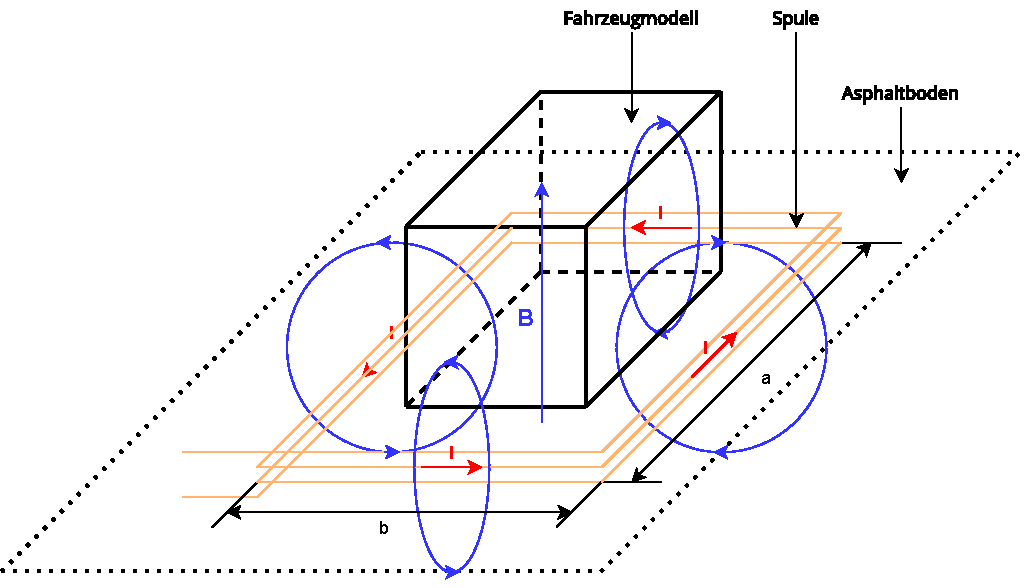
\includegraphics[width=1\linewidth]{fahrzeugerkennung/Spuleninstallation.pdf}
    \caption{Installation der Spule}
  \end{figure}
  Dieses Messkonzept zusammen mit der Installation der Spule im Boden bietet folgende Vorteile.

\begin{comment}

Bis auf die relative Permeabilität sind alle anderen Variablen konstant. Daraus lässt sich schlussfolgern, dass der magnetische
Fluss $\Phi$ anhand der Gleichung \ref{eq:phi} und \ref{eq:Rm} proportional zur relativen Permeabilität ist. 




\begin{equation} \label{iq:phi}
    \Phi \propto \mu_{r}
\end{equation}
Der Fluss $\Phi$ hängt somit auch von den Materialien ab durch die er fließt. In der nächsten Abbildung kann man erkennen,
wie ein Fahrzeug über eine im Boden installierte Spule den magnetischen Fluss $\Phi$ und somit die magnetische Flussdichte $B$
beeinflussen kann. 

\begin{figure}[H]
    \centering
    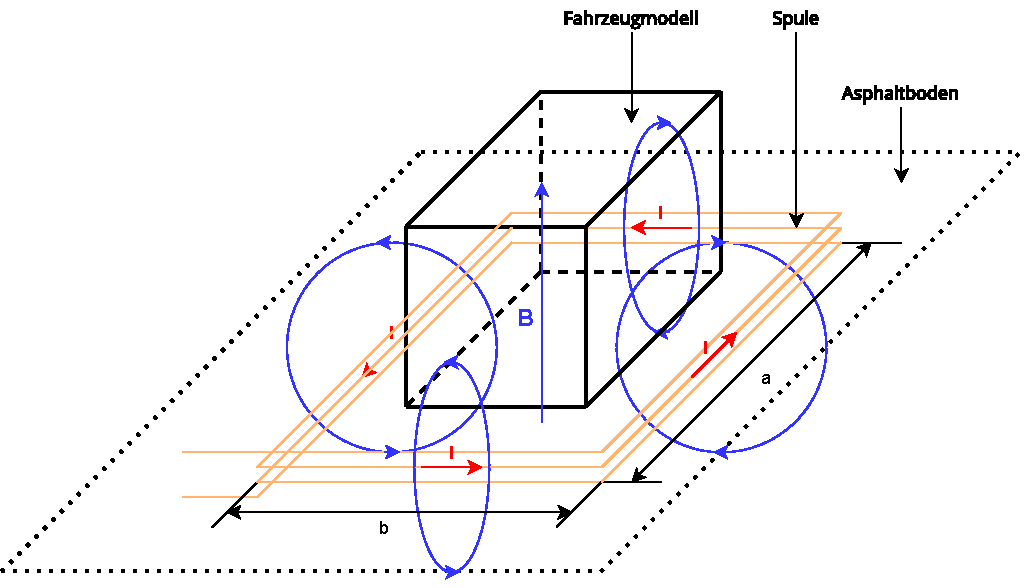
\includegraphics[width=1\linewidth]{fahrzeugerkennung/Spuleninstallation.pdf}
    \caption{Installation der Spule}
  \end{figure}
Um diese Größen auslesbar zu machen, müssen diese magnetischen Größen bei einer direkten Messung in elektrische Größen umgewandelt
werden.
Hierfür gelten folgende Zusammenhänge:

\begin{equation} \label{eq:L_phi}
    L = \frac{N \cdot \Phi}{I} = \frac{\Psi}{I} 
\end{equation}
Wobei \\
$L$ = Induktivität der Spule \\
$I$ = Strom der durch die Spule fließt \\
$N$ = Anzahl der Windungen der Spule \\
$\Psi$ = Verkettete Fluss

\pagebreak
\begin{equation} \label{eq:L_i}
    u(t) = L \cdot \frac{di(t)}{dt}
\end{equation}

Wobei \\
$L$ = Induktivität der Spule \\
$i(t)$ = Strom der durch die Spule fließt zum Zeitpunkt t \\
$u(t)$ = Spannung die an der Spule anliegt zum Zeitpunkt t \\
$t$ = Zeit in s \\
So lässt sich bei Bekanntheit von Strom und Spannung auf die Induktivität und mit der Gleichung \ref{eq:L_phi} 
und mit dem Zusammenhang \ref{iq:phi} auf die magnetischen Eigenschaften des Materials rückschließen. 
Diese Art der Detektion bietet viele praktische Vorteile.
\end{comment}
\begin{itemize}
    \item \textbf{Größerer Messbereich} \\
    Im Vergleich zu anderen Detektionsmethoden wie einer Leichtschranke kann man einen größeren Bereich durch die Wirkfläche
    der Spule abdecken. So lassen sich auch kleinere Kraftfahrzeuge wie Motorräder oder Mopeds besser erkennen.
    \item \textbf{Schutz vor Umweltfaktoren} \\
    Durch den Verbau im Boden ist die Messeinrichtung vor Umwelteinflüssen wie Regen, Frost, hohen beziehungsweise
    niedrigen Temperaturen und Korrosion besser geschütz. Dies verringert auch den Einfluss dieser Störfaktoren auf die Eigenschaften
    Spule und somit auf die daraus resultierenden Messergebnisse.
    \item \textbf{Ausschließung von Materialien} \\
    Alle nicht metallische Stoffe werden von diesem Messprinzip nicht wahrgenommen. So können Verschmutzungen wie Blätter und Staub, welche
    visuelle Sensoren stören können, die Detektion nicht behindern. Es können sich jedoch Effekte, die den magnetischen Widerstand anheben und senken, 
    einander aufheben. 
    
\end{itemize}
\subsubsection{Messung ferromagnetischer Metalle}
Um dieses Detektionsverfahren zu verstehen muss zuerst der Zusammenhang zwischen Induktivität und relativer Permeabilität verstanden werden.
Aus den Gleichungen \ref{eq:Rm}, \ref{eq:phi} und \ref{eq:L_phi} kann die folgende Proportionalität ermittelt werden:
\begin{equation} \label{iq:L_mu}
    L \propto \mu_{r}
\end{equation}
Bei ferromagnetischen Stoffen wie Eisen ist die relative Permeabilität sehr viel größer als 1. Wenn nun ein Auto oder 
ein anderes Fahrzeug sehr viel Eisen beinhaltet wirkt sich dies steigernd auf die Induktivität der Spule aus. Die folgenden
Verfahren nutzen dieses Prinzip, um die Belegung einer Parklücke zu bestimmen.

\paragraph{RL-Oszillator mit Timer Baustein}\mbox{}

Bei diesem Messverfahren wird die Änderung der Induktivität $L$ über die Änderung einer Stromladekurve über einen Widerstand
$R$ ermittelt. Eine Simulation in LTSpice mit folgendem Schaltbild kann die Auswirkung auf eine Ladekurve bei gleicher Spannung
und gleichem Widerstand gut darstellen.
\begin{figure}[H]
    \centering
    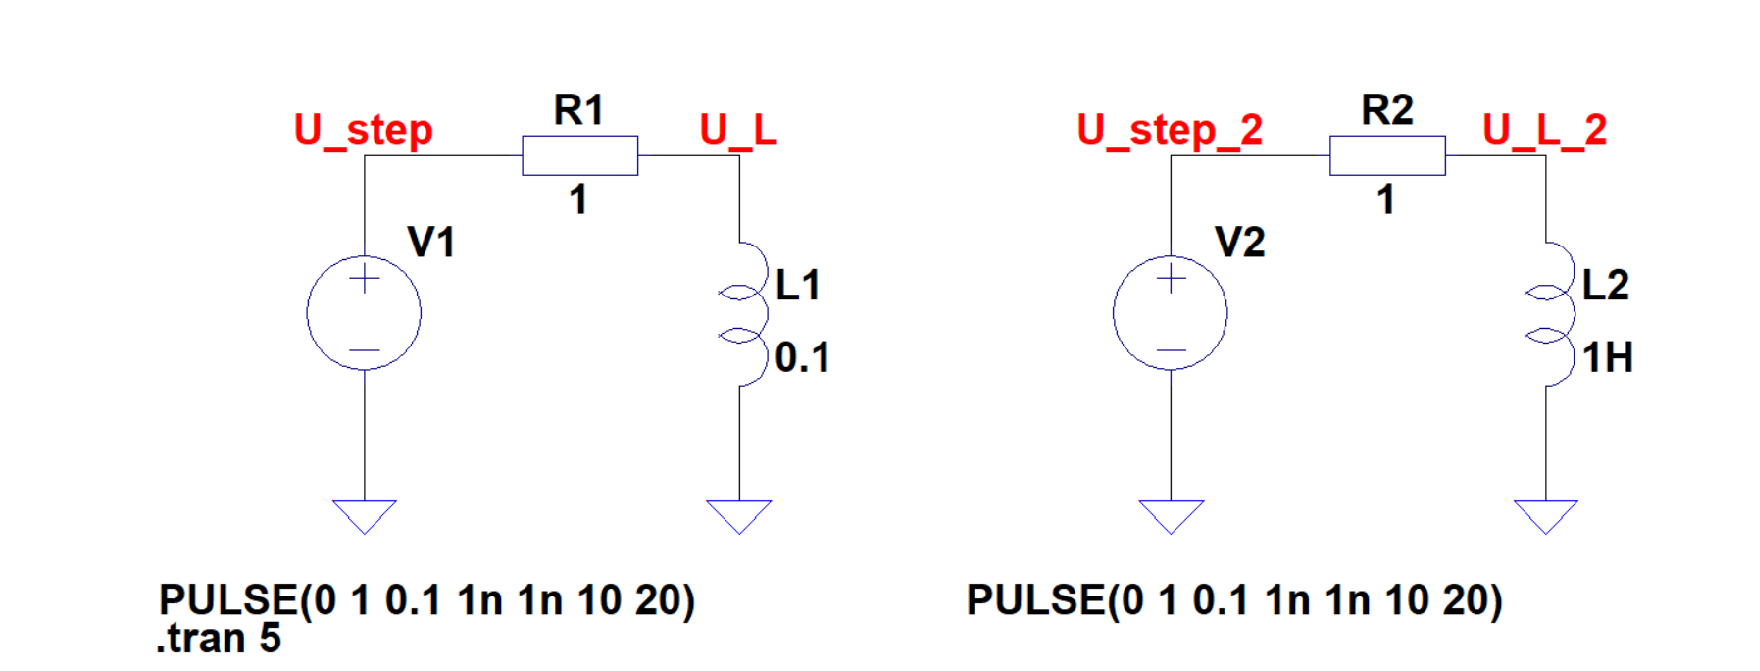
\includegraphics[width=1\linewidth]{fahrzeugerkennung/Ladekurven.pdf}
    \caption{LTSpice Blockbild zweier RL-Glieder}
\end{figure}
\pagebreak
Die daraus resultierende Simulation im Zeitbereich ergibt folgendes Ergebnis:

\begin{figure}[H]
    \centering
    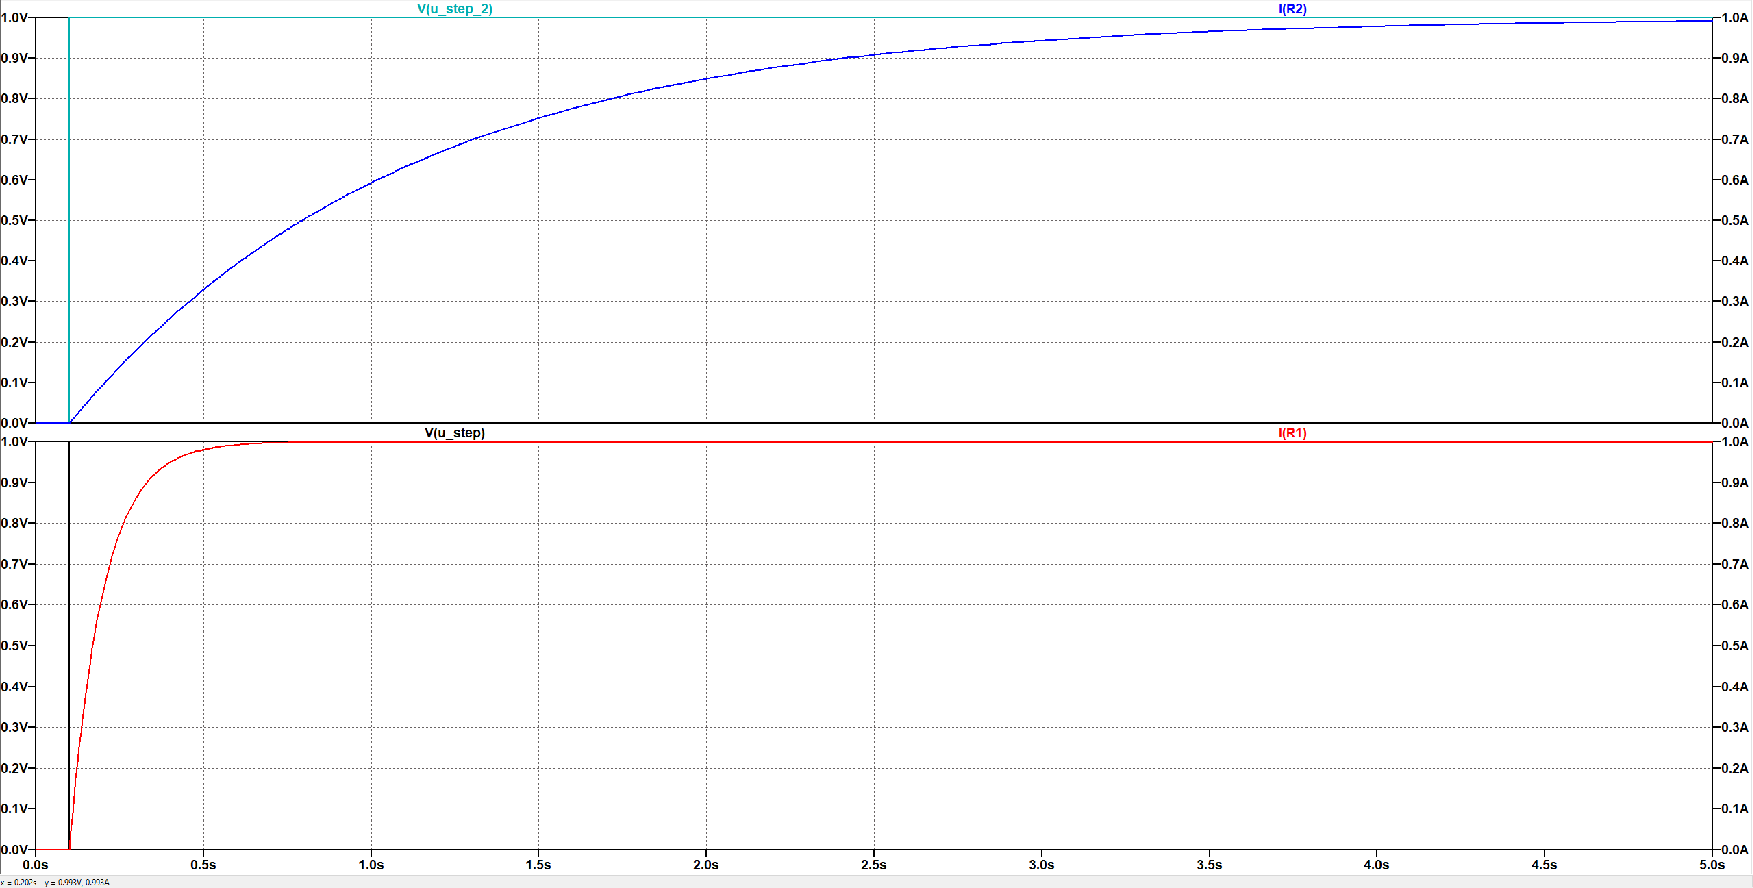
\includegraphics[width=1\linewidth]{fahrzeugerkennung/Ladekurven_ZB.pdf}
    \caption{Stromkurven zweier RL-Glieder}
\end{figure}

Es ist aus der letzten Abbildung erkennbar, dass sich eine größere Induktivität verlangsamend auf die Zunahme des Stromes auswirkt. Für Einschaltvorgänge kann diese Stromkurve
für RL-Glieder folgendermaßen beschrieben werden.

\begin{equation} \label{eq:i_L}
    i(t) = \frac{U_{0}}{R} \cdot (1 - e^{-\frac{t}{\tau}})
\end{equation}

\begin{equation} \label{eq:tau_RL}
    \tau = \frac{L}{R}
\end{equation} 

Wobei \\
$i(t)$ = Strom der durch die Spule fließt zum Zeitpunkt t \\
$L$ = Induktivität der Spule in H\\
$R$ = Widerstand in $\Omega$ \\
$U_0$ = Spannung die nach dem einschalten anliegt in V\\
$t$ = Zeit in s \\
$\tau$ = Zeitkonstante in $\frac{1}{s}$\\

Timer Bausteine wie der NE555 nutzen solche Verlaufskurven wenn sie als astabile Kippstufe konfiguriert sind.
Es gibt einen Eingang dieses Baustein meist CV für Control Voltage der die Spannung überwacht. Überschreitet diese Spannung zwei Drittel
der Betriebsspannung schaltet er einen weiteren Pin, meist DIS für Discharge, auf 0V beziehungsweise auf Masse. Unterschreitet jedoch 
die Spannung am CV Pin ein Drittel der Betriebsspannung so wird der DIS Pin auf Betriebsspannung geschalten. Diese beiden Pins 
sind über RC- oder RL- Glieder verbunden. Es entsteht somit ein Oszillator, welcher die Spannung am DIS Pin anhebt und absenkt.
Der NE555 kann dieses Signal über einen internen Komparator in ein Rechtecksignal umwandeln, welches besser von Mikrocontrollern ausgelesen
werden kann. Der Mikrocontroller kann so die Anzahl der einkommenden Takte über einen gewissen Zeitraum zählen und daraus eine Oszillatorfrequenz errechnen.
Die Zeitsignale lassen sich in LTSpice mit dem NE555 als Timer-Baustein simulieren.

\begin{figure}[H]
    \centering
    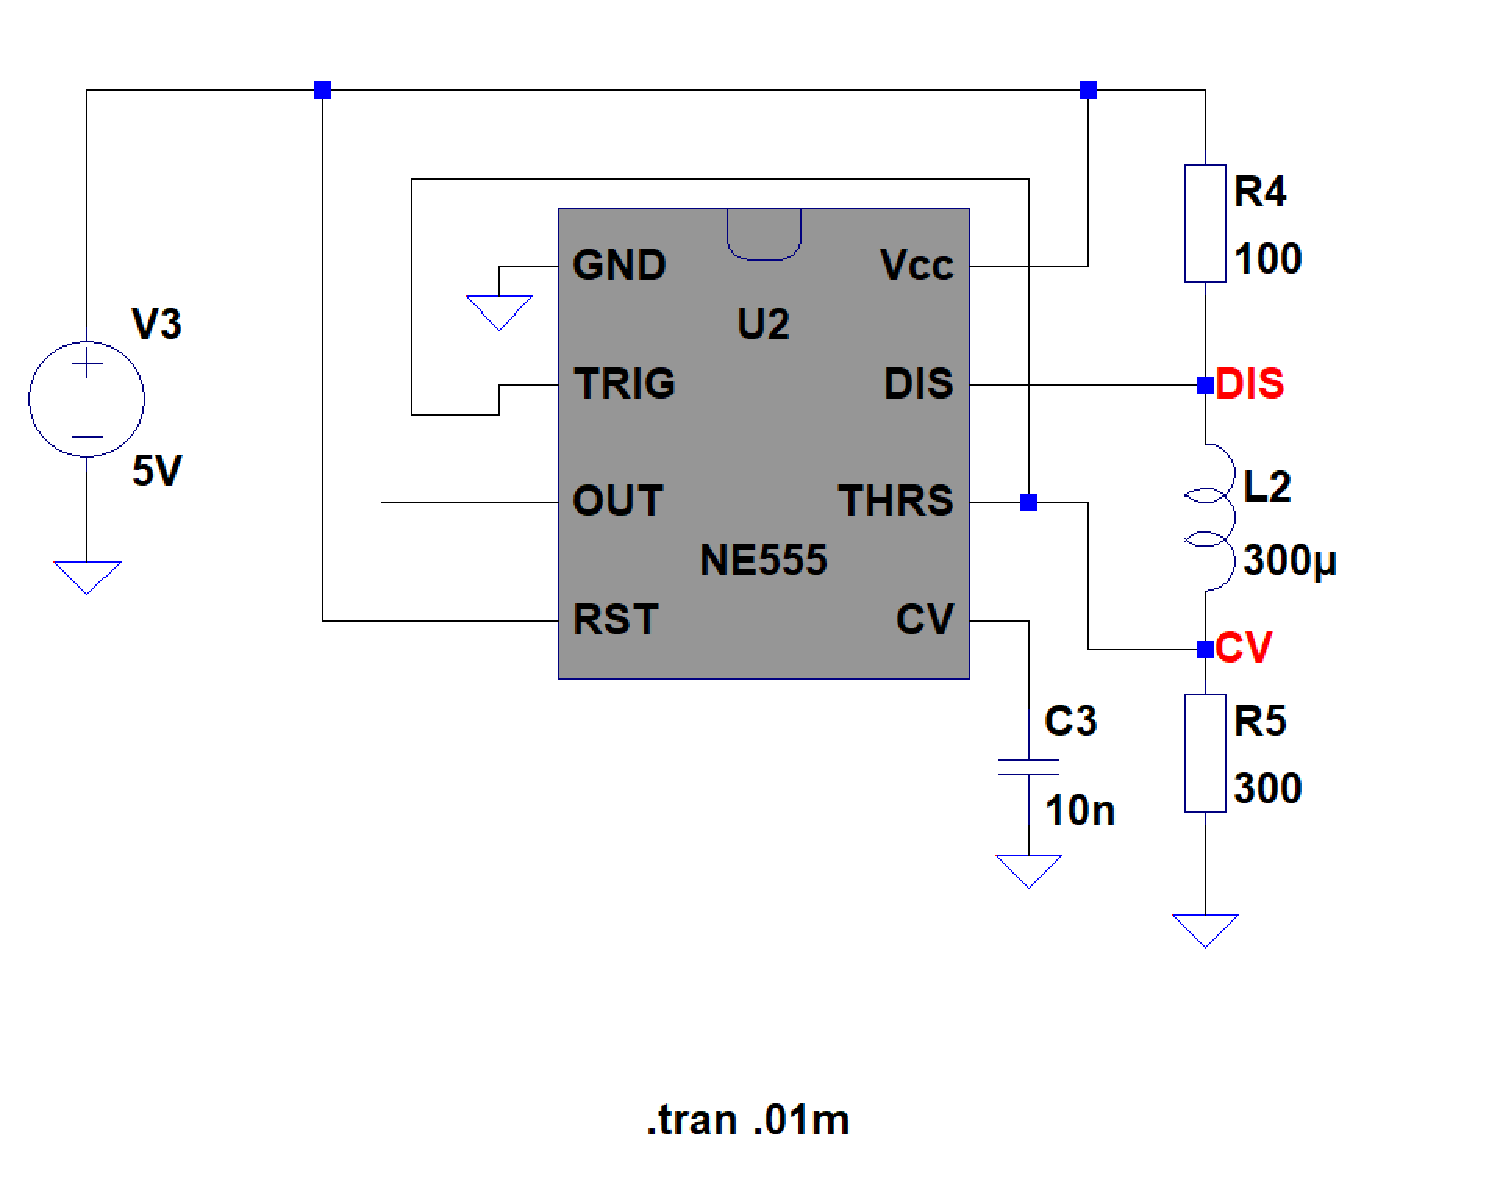
\includegraphics[width=0.6\linewidth]{fahrzeugerkennung/RL_Oszillator.pdf}
    \caption{RL-Oszillator mit NE555}
\end{figure}

\begin{figure}[H]
    \centering
    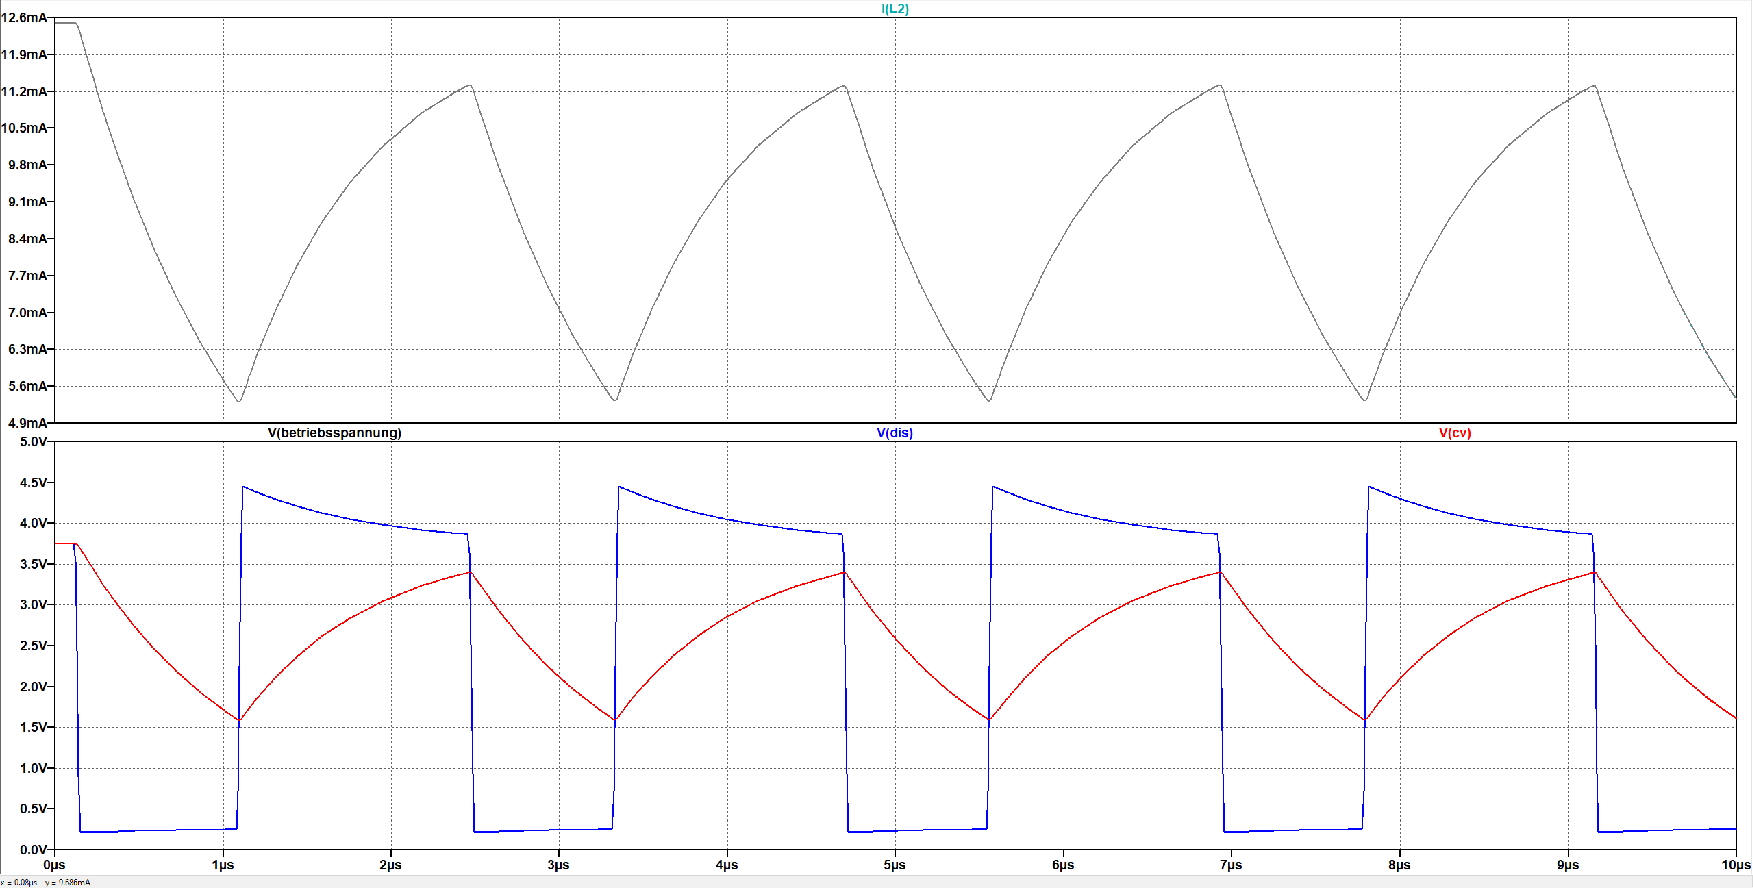
\includegraphics[width=1\linewidth]{fahrzeugerkennung/RL_Oszillator_ZB.pdf}
    \caption{RL-Oszillator mit NE555 Zeitsignale}
\end{figure}

Im oberen Diagramm ist der Verlauf des Stromes durch die Spule zu erkennen, der wie erwartet zu- und abnimmt. Im unteren Diagramm ist in 
schwarz die Betriebsspannung als Referenz, in Rot der CV Pin und in Blau der DIS Pin des NE555. Das rote Signal wechselt zwischen zwei Drittel der Betriebsspannung 
und einem Drittel der Betriebsspannung mit einer Frequenz von $f = \SI{438}{\kilo\hertz}$ bei einer Induktivität von $L = \SI{300}{\micro\henry}$, einem Widerstand $R4 = 100\Omega$ und einem
Widerstand $R5 = 300\Omega$. Die Simulation entspricht hier der Theorie, jedoch bricht das blaue Signal am Pin DIS in der Einschaltphase ein.
Der Grund dafür ist der interne Widerstand des NE555, der ab einem gewissen Stromverbrauch für einen Spannungsabfall sorgt. Da es meist besser ist mit
niedrigen Frequenzen zu arbeiten, ist es nach den Gleichungen \ref{eq:i_L} und \ref{eq:tau_RL} entweder nötig die Induktivität zu erhöhen oder die Widerstände zu verkleinern.
Die Induktivität lässt sich entweder durch Erhöhen der Windungen oder durch Vergrößerung der Spule erreichen steigern, was in vielen Fällen nicht möglich ist oder kostspielig wird.
Die Reduktion der Widerstände führt zu einer Zunahme des Stromes und der Verlustleistung, was auch unerwünscht ist.
Aus diesen Gründen ist der RL-Oszillator nur für hohe Frequenzen geeignet. In der nächsten Abbildung sieht man die Zeitsignale bei verschiedenen Induktivitäten
nämlich bei $L2 = \SI{100}{\micro\henry}$ und bei $L2 = \SI{1}{\milli\henry}$

\begin{figure}[H]
    \centering
    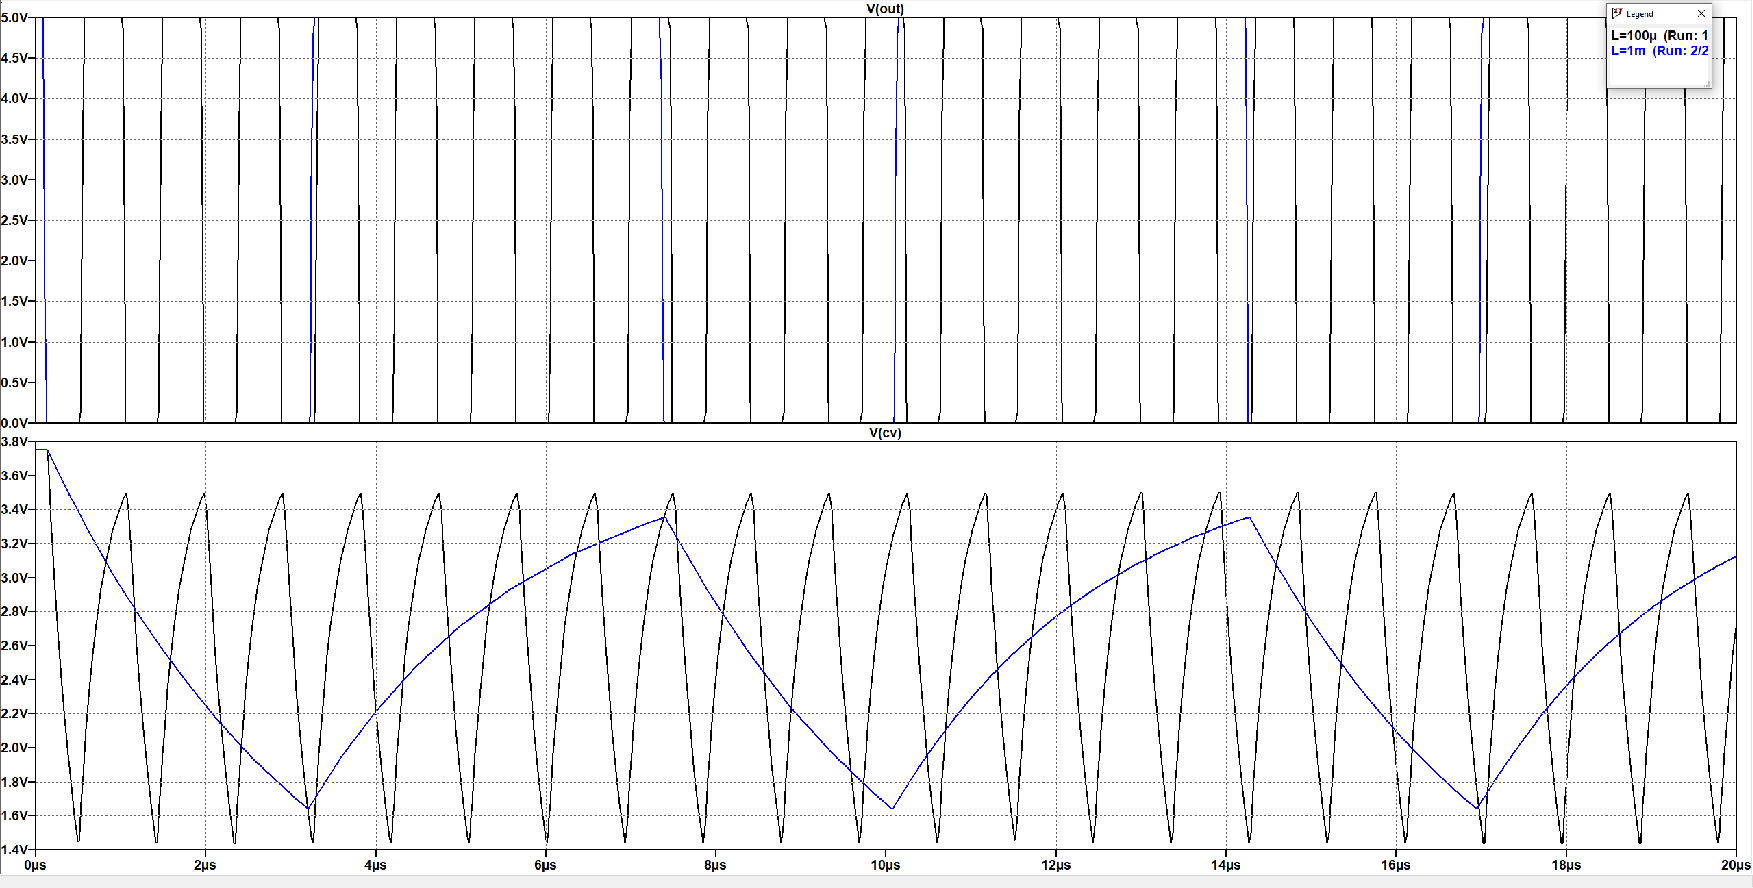
\includegraphics[width=1\linewidth]{fahrzeugerkennung/RL_Oszillator_vergleich2_ZB.pdf}
    \caption{Vergleich des NE555-Oszillators bei unterschiedlichen L}
\end{figure}

Eine Verzehnfachung der Induktivität führt zu einer Reduktion der Oszillatorfrequenz um den Faktor 10.
So kann eine Änderung des magnetischen Widerstands über die Induktivität auf eine Frequenz umgewandelt werden. Diese Frequenz kann dann sehr genau von einem
Mikrocontroller bestimmt werden. 

\begin{equation} \label{iq:f_NE555}
    f \propto \frac{1}{L}
\end{equation} 

\pagebreak
\subsubsection{Messung paramagnetischer Metalle}
Da nicht alle Metalle ferromagnetische Eigenschaften haben werden viele Stoffe wie Aluminium, Kupfer oder diverse Legierungen
von einer niederfrequenten Messung der Induktivität nicht wahrgenommen. Ein Effekt, welcher bei elektrischen Leitern Abhilfe schaffen kann, sind 
die Eddy Currents. Wenn in einem Leiter ein magnetisches Feld einwirkt, induziert dieses im Objekt Ströme, die wiederum ihr eigenes magnetische Feld erzeugen.
Die fließenden Ströme erzeugen im Objekt Ohmsche Verluste und das System wirkt wie ein belasteter Transformator. Die Stromaufnahme der Spule steigt also durch die Anwesenheit
des Leiters auf der Parklücke und wirkt somit den Effekten eines ferromagnetischen Materials entgegen.

\begin{comment}
    welche normalerweise unerwünscht sind. Sie wirken auch einer Änderung des magnetischen Feldes entgegen,
da sie selbst Energie brauchen um ihre Richtung zu ändern. Je größer die Frequenz der eingespeisten Felddichte $B$ desto stärker wirkt die 
Flussdichte $B_{eddy}$ senkend auf die Gesamtflussdichte und so auf den magnetischen Fluss $\Phi$. 
Nach der Gleichung \ref{eq:L_phi} reduziert sich die Induktivität mit zunehmender Frequenz.
\end{comment}




\begin{figure}[H]
    \centering
    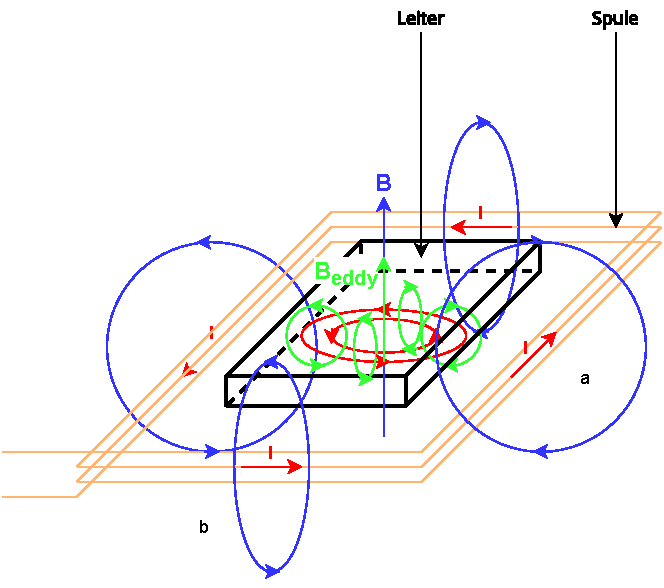
\includegraphics[width=0.6\linewidth]{fahrzeugerkennung/Eddy_Currents.pdf}
    \caption{Eddy Currents in einem Leiter}
\end{figure}

Bei sehr hohen Frequenzen ist jedoch zu beachten, dass der Skin-Effekt die Querschnittsfläche, durch die der Wechselstrom fließen kann,
reduziert. Somit nimmt der Effekt der Eddy-Currents ab. Diese Phänomene werden jedoch nicht in dieser Arbeit behandelt, da sie außerhalb des Rahmens der 
Fahrzeugerkennung liegen. 

\paragraph{LC Oszillatoren}\mbox{}

Im Vergleich zum RL-Oszillator, der über eine astabile Kippstufe lauft, kann ein LC Oszillator seine Resonanzfrequenz nur durch das Verstellen der Induktivität und der Kapazität 
eines Kondensators verändern. Zudem gibt es in der Theorie keine Wirkverluste, da die Energie abwechselnd zwischen magnetischer und elektrischer Energie umgewandelt wird. In der Realität gibt es jedoch
ohmsche Verluste, die zu einem Abklingen der Schwingung führen. Es braucht daher ein aktives Glied wie ein Transistor oder ein Operationsverstärker, der den Oszillator mit Energie versorgt.
\\
Der zeitliche Verlauf einer ungedämpften Schwingung kann in LTSpice simuliert werden indem wir eine Sprungfunktion auf ein LC Glied geben und einen Widerstand in Serie zum Kondensator oder zur
Spule geben.

\begin{figure}[H]
    \centering
    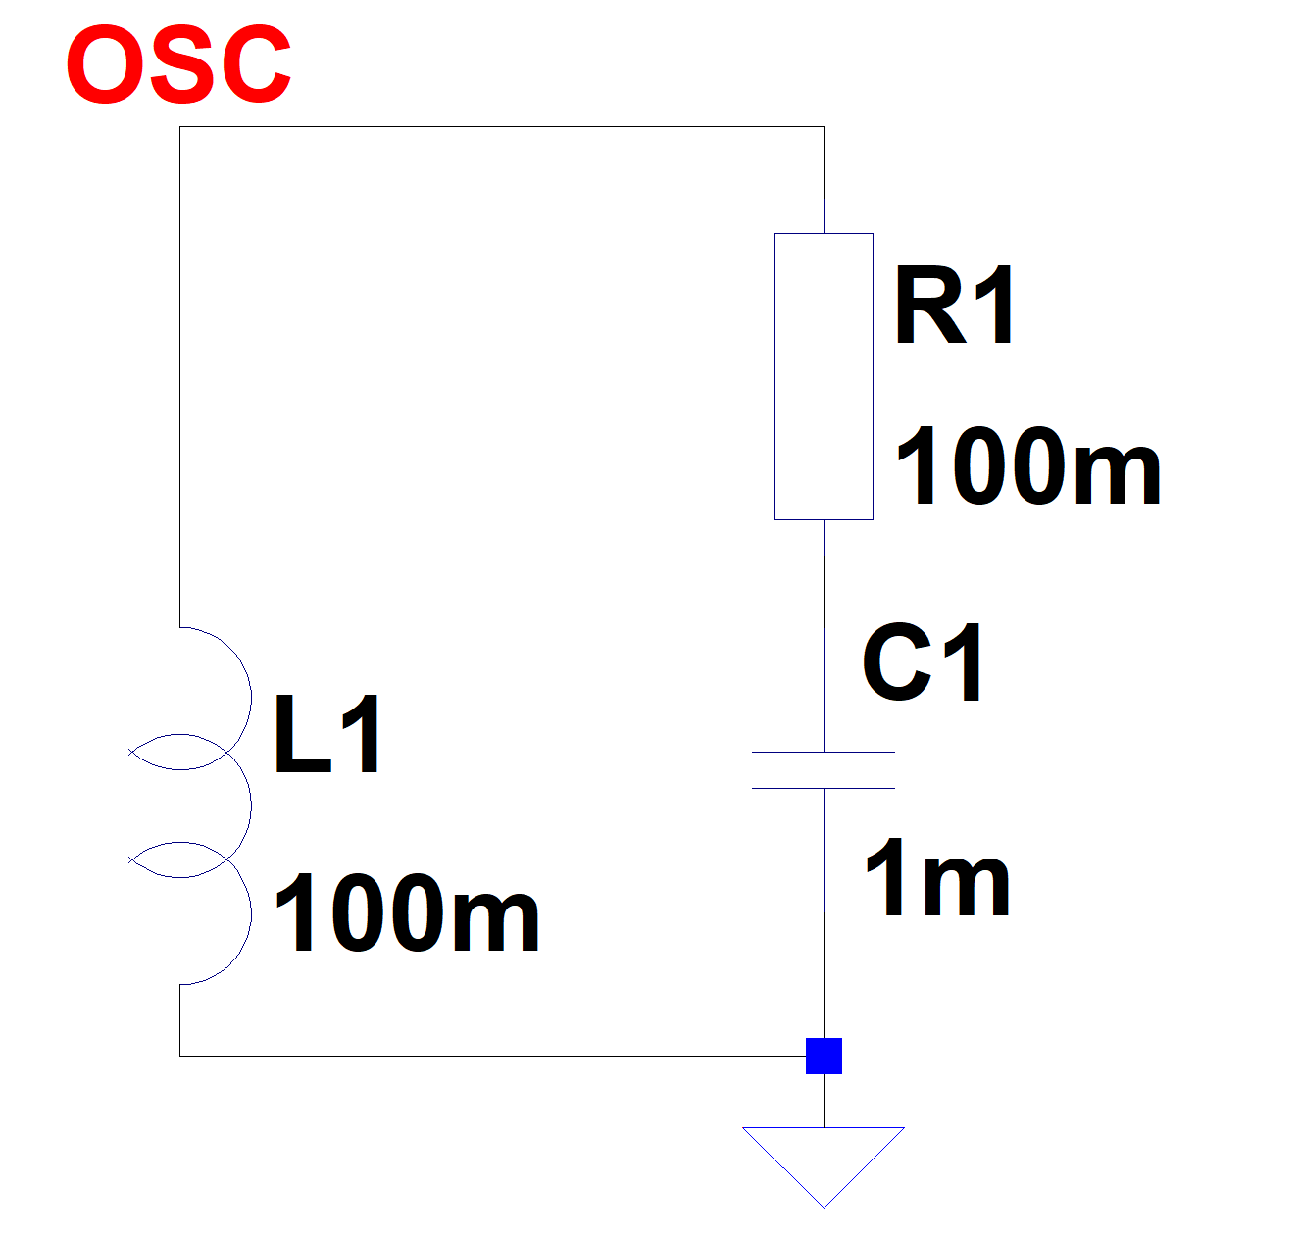
\includegraphics[width=0.6\linewidth]{fahrzeugerkennung/LC_Parallel.pdf}
    \caption{Parallelschwingkreis in LTSpice}
\end{figure}

\begin{figure}[H]
    \centering
    \includegraphics[width=1\linewidth]{fahrzeugerkennung/gedämpfte_schw.pdf}
    \caption{Gedämpfte Schwingung}
\end{figure}

Aus der Simulation ergibt sich über eine Cursormessung für die angegebenen Werte $L = \SI{100}{\milli\henry}$ und $C = \SI{100}{\milli\farad}$ eine Resonanzfrequenz von $f = \SI{15,85}{\hertz}$. Die Resonanzfrequenz für einfache LC-Schwingkreise lässt sich mit der
Thomsonschen Schwingungsgleichung errechnen:

\begin{equation} \label{eq:thomson}
    f = \frac{1}{2 \cdot \pi \sqrt{L \cdot C}}
\end{equation}

Wobei \\
$f$ = Resonanzfrequenz des LC-Gliedes\\
$L$ = Induktivität der Spule\\
$C$ = Kapazität des Kondensators\\

Wenn man die Werte $L = \SI{100}{\milli\henry}$ und $C = \SI{100}{\milli\farad}$ in die Gleichung \ref{eq:thomson} einsetzt erhält man eine Resonanzfrequenz von $f = 15.915Hz$.
Allgemein tritt in LC-Glieder bei einer Phasenlage von $\varphi_{LC} = 180^{\circ}$ und bei der Frequenz nach der Thomsonschen Gleichung \ref{eq:thomson}  Resonanz auf. 

\paragraph{Einfluss von Induktivitätsänderungen auf LC-Oszillatoren}\mbox{}

Für die Fahrzeugerkennung ist es von Relevanz zu wissen wie die Frequenz dieser Oszillatoren auf die Änderung der Induktivität der im Boden verbauten Spule reagiert.
Wenn eine Parklücke frei ist besitzt die Spule eine Induktivität von $L_{0}$ und hat nach der Thomsonschen Gleichung \ref{eq:thomson} eine Resonanzfrequenz $f_{0}$. Für kleine Änderungen $\Delta L$ kann eine Näherung
der Frequenzänderung gemacht werden indem man in den Punkt $(f_{0}, L_{0})$ in den Graphen der Thomsonschen Gleichung aufgetragen über die Induktivität $L$ eine Tangente in diesen Punkt legt. Bei einer 
Kapazität von $C = \SI{1}{\micro\farad}$ erhält man folgenden Graphen: 

\begin{center}
    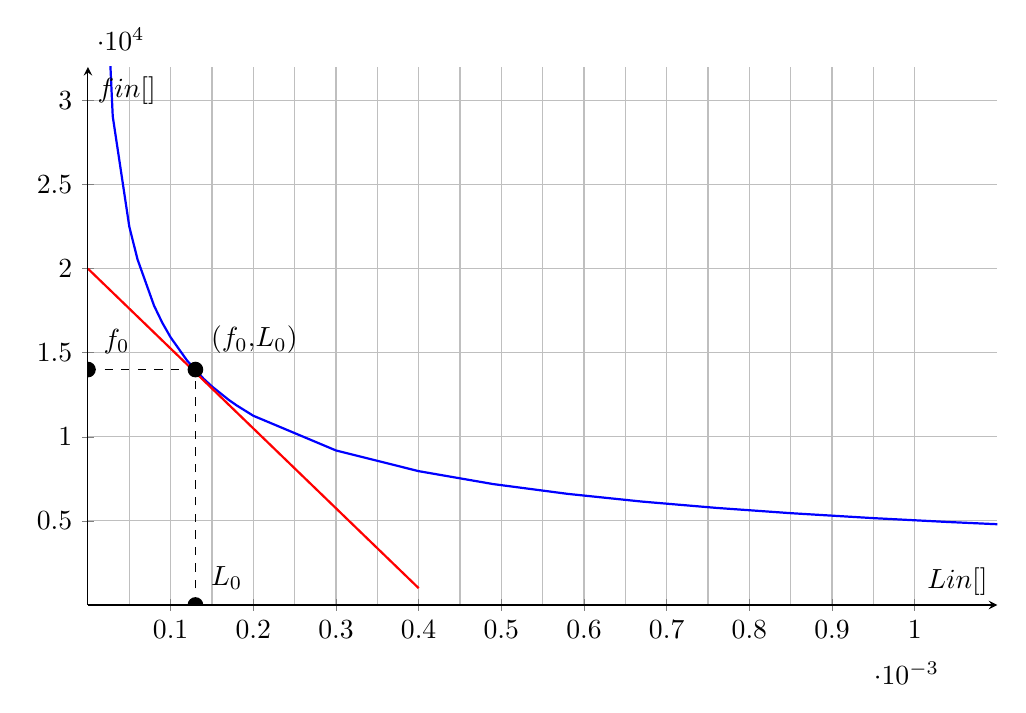
\begin{tikzpicture}
        
        \begin{axis}[
                axis x line=middle, 
                axis y line=middle, 
                xlabel={$L \text{ in } \si[]{\henry}$}, 
                ylabel={$f \text{ in } \si[]{\hertz}$}, 
                x=15cm/0.001,    
                y=0.0003cm,    
                grid =both,
                minor x tick num=1,
                subtickwidth=0pt,
                xtick={0,0.0001,...,0.001}, 
                ytick={0,5000,...,30000}, 
                xmin=0,  
                xmax=0.0011,   
                ymin=0,  
                ymax=32000,  
                scale = 0.7 
        ]
        
        \addplot [blue, thick, samples at={0,0.000001,0.000005,0.00001,...,0.0002,0.0003,0.0004,...,0.002}] {1/(2*pi*sqrt(x*1e-6))};
        \addplot[mark=none, red, thick] coordinates {(0, 20000) (0.4e-3, 0.1e4)};
        \addplot[mark=none, black, dashed] coordinates {(0, 1.4e4) (0.13e-3, 1.4e4)};
        \addplot[mark=none, black, dashed] coordinates {(0.13e-3, 0) (0.13e-3, 1.4e4)};
        \node[label={45:{($f_{0}$,$L_{0}$)}},circle,fill,inner sep=2pt] at (axis cs:0.13e-3,1.4e4) {};
        \node[label={45:{$L_{0}$}},circle,fill,inner sep=2pt] at (axis cs:0.13e-3,0) {};
        \node[label={45:{$f_{0}$}},circle,fill,inner sep=2pt] at (axis cs:0,1.4e4) {};
    \end{axis}
    \end{tikzpicture}
\end{center}

Mit dieser Näherung kann man mit Hilfe des Differentials der Thomsonschen Gleichung \ref{eq:thomson} die Änderung des Funktionswertes $f(L \pm \Delta L) = \Delta f \approx df$ bestimmt werden.
\begin{align*} \label{eq:df_L}
    df = \frac{\partial f}{\partial L}\bigg|_{L_{0}} \cdot dL \\ 
    df = \frac{\partial}{\partial L}  \left (  \frac{1}{2 \pi \sqrt{L_{0}C}} \right ) \Delta L \\
    df = - \frac{1}{4 \pi} (L_{0}C)^{-\frac{3}{2}} \cdot \Delta L
\end{align*}

Für relative Änderungen der Induktivität $\Delta L$ um den Wert $L_{0}$ gilt:

\begin{equation} \label{eq:f_df}
    \frac{df}{f_{0}} =  -\frac{1}{2C} \cdot \frac{\Delta L}{L_{0}}
\end{equation}

Das bedeutet, dass eine kleine relative Änderung der Inuktivität $\frac{\Delta L}{L_{0}}$ bei gleicher Kapazität $C$ für eine halb so große relative Änderung in der Frequenz führt. 
Dieser Ansatz gilt nur bei kleinen $\Delta L$.

\paragraph{Messung der Frequenz eines Colpitts-Oszillator}\label{sec:colpitts}\mbox{}

Der Colpitts-Oszillator ist eine Variante des LC-Oszillator und wird in der Praxis oft mit einem aktiven Element betrieben. Im Vergleich zu einem einfachen LC-Glied besitzt dieser Oszillator
zwei Kondensatoren. Das Schaltbild sieht so aus:

\begin{figure}[H]
    \centering
    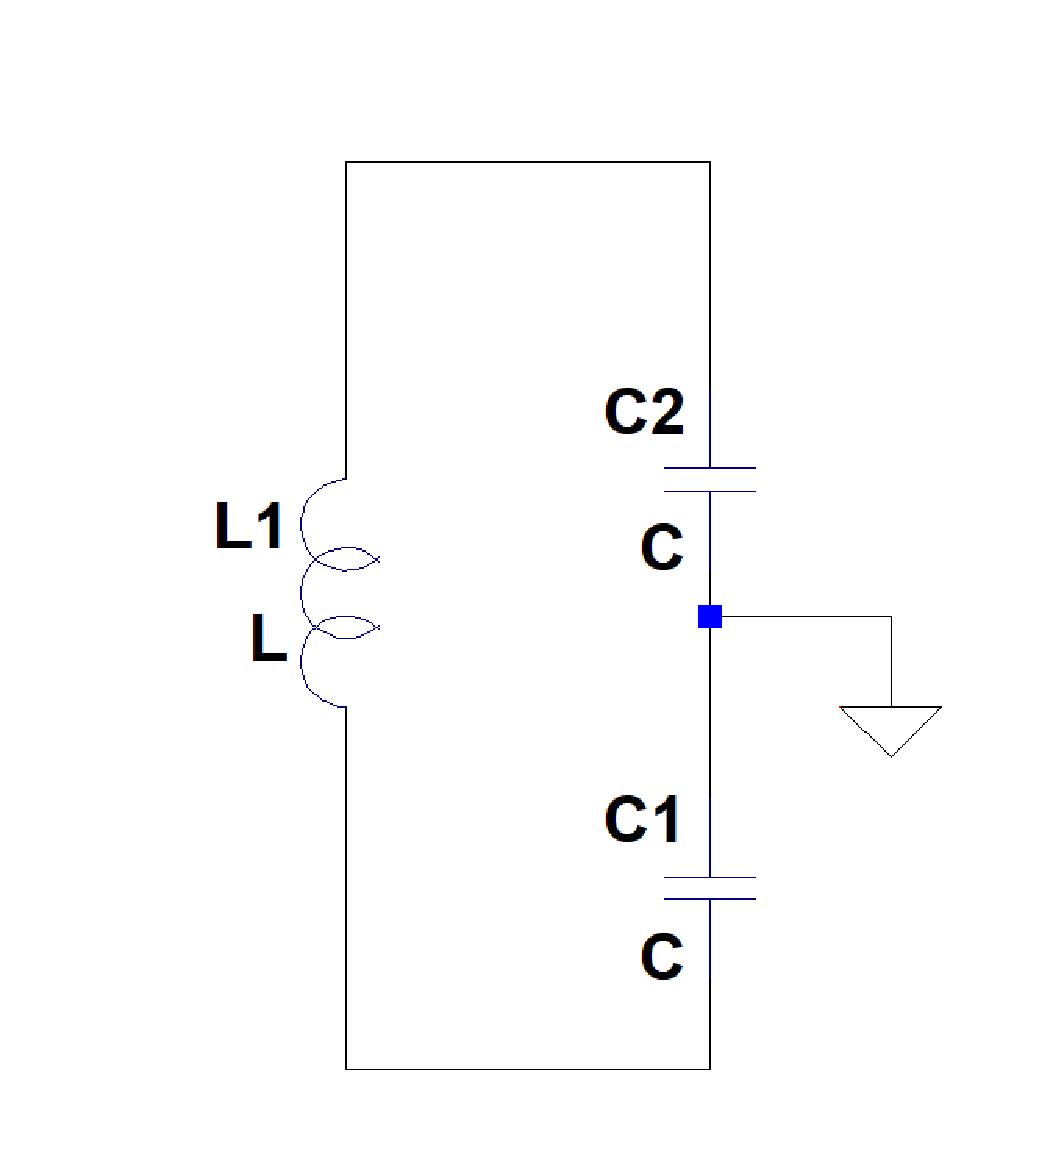
\includegraphics[width=0.3\linewidth]{fahrzeugerkennung/Colpitts_LC.pdf}
    \caption{Colpitts LC-Glied}
\end{figure}

Dieses LC-Glied wird als Rückkoppelglied eingesetzt und sorgt für die nötige Phasendrehung von $\varphi_{LC} = 180^{\circ}$. Wie man in der obigen Abbildung sehen kann liegen die Kondensatoren 
$C_{1}$ und $C_{2}$ in Serie. Es ergibt sich daher eine Gesamtkapazität von $C_{ges}$.

\begin{equation} \label{eq:c_gescolpitts}
    C_{ges} = \frac{C_{1} \cdot C_{2}}{C_{1} + C_{2}}
\end{equation}
Durch Einsetzen in die Thomsonsche Gleichung erhält man für die Resonanzfrequenz eines Colpitts-Oszillator:
\begin{equation} \label{eq:colpitts}
    f = \frac{1}{2 \cdot \pi \sqrt{L \cdot \left( \frac{C_{1} \cdot C_{2}}{C_{1} + C_{2}} \right) }}
\end{equation}

Wobei \\
$f$ = Resonanzfrequenz des Colpitts-Oszillator\\
$L$ = Induktivität der Spule\\
$C_{1}$ = Kapazität des Kondensators $C_{1}$\\
$C_{2}$ = Kapazität des Kondensators $C_{2}$\\

\pagebreak
Das aktive Element wird an die Anschlüsse der Spule angeschlossen und muss selbst eine Phasendrehung von 180° liefern. Zusätzlich muss die Verstärkung des Gliedes größer als 1 sein damit eine dauerhafte 
Schwingung entstehen kann. Mit einem Operationsverstärker muss der nicht invertierende Eingang auf eine Bezugsspannung gelegt werden. Diese Bezugsspannung wird oft in die Mitte des Versorgungsspannungsbereich
gelegt. Bei einem Spannungsbereich von $\SI{0}{\volt}$ bis $\SI{5}{\volt}$ ist eine Bezugsspannung von $\SI{2,5}{\volt}$ sinnvoll. Der invertierende Eingang wird an das Colpitts LC-Glied angeschlossen. Der Ausgang des Operationsverstärker wird über
einen Widerstand an das LC-Glied geschalten, damit das Rückkoppelglied besser vor Übersteuerungen am Ausgang des Operationsverstärkers geschützt ist. 

\begin{figure}[H]
    \centering
    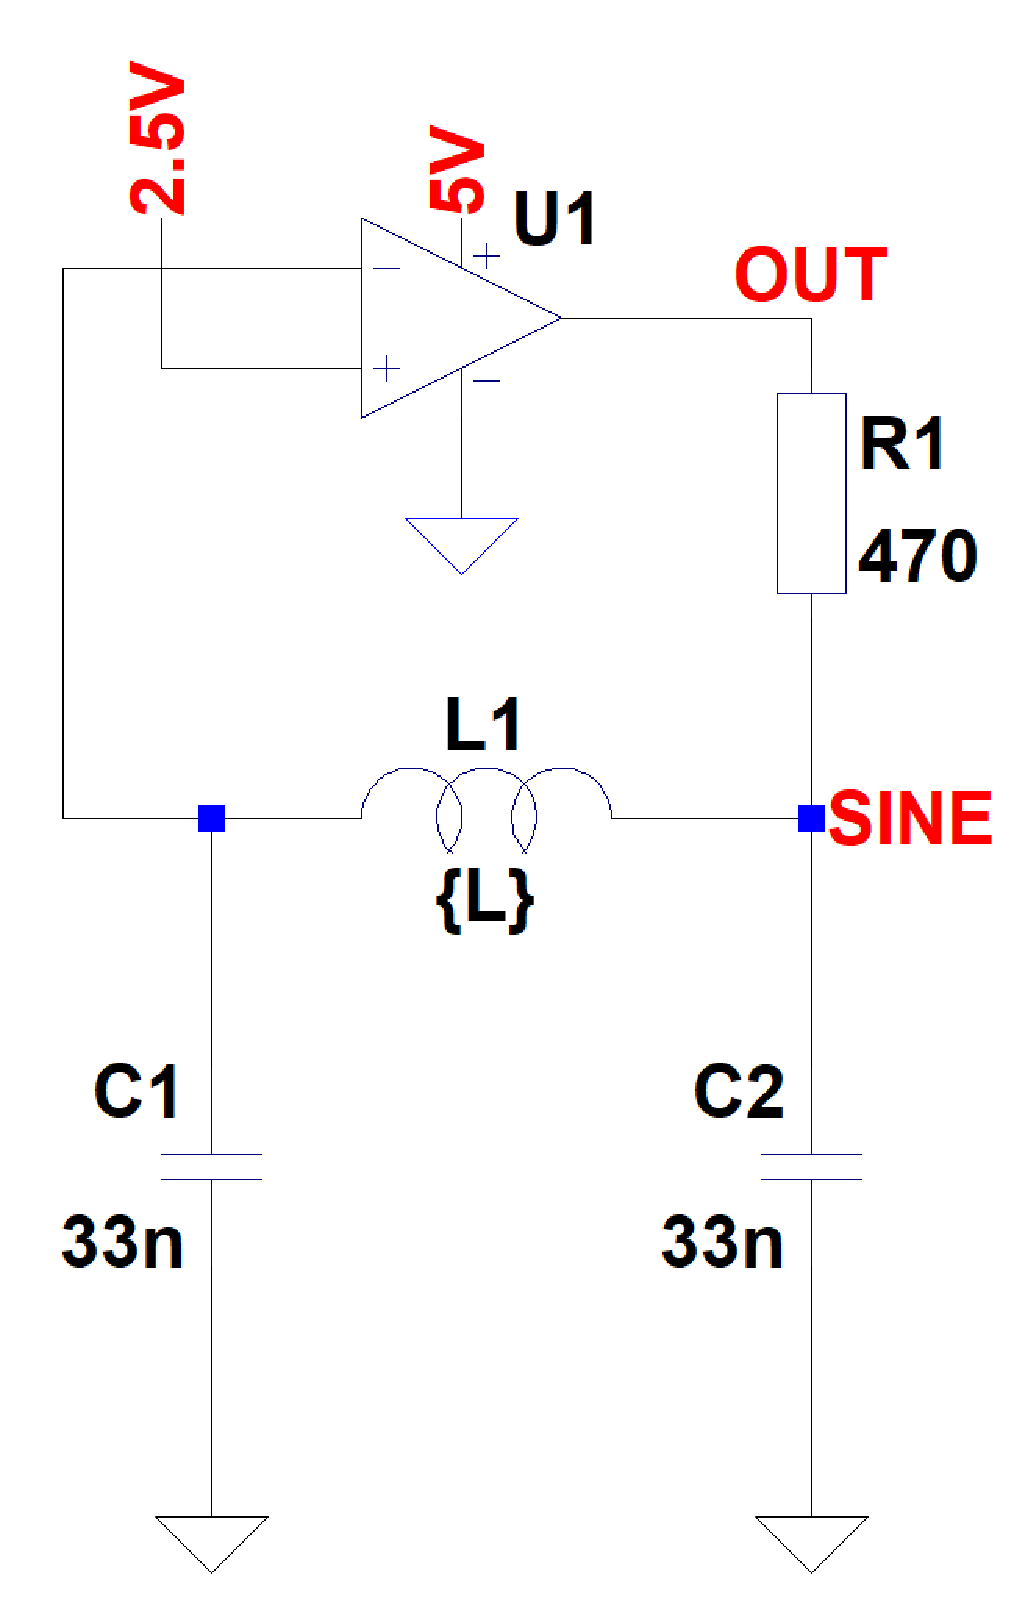
\includegraphics[width=0.4\linewidth]{fahrzeugerkennung/Colpitts_active.pdf}
    \caption{Aktiver Colpitts-Oszillator}
\end{figure}

Wenn man nun verschiedene Werte für die Induktivität einsetzt ergeben sich durch die Simulation dieses Schaltbildes folgende Zeitsignale für den Ausgang des Operationsverstärker OUT und der Spannung SINE:

\begin{figure}[H]
    \centering
    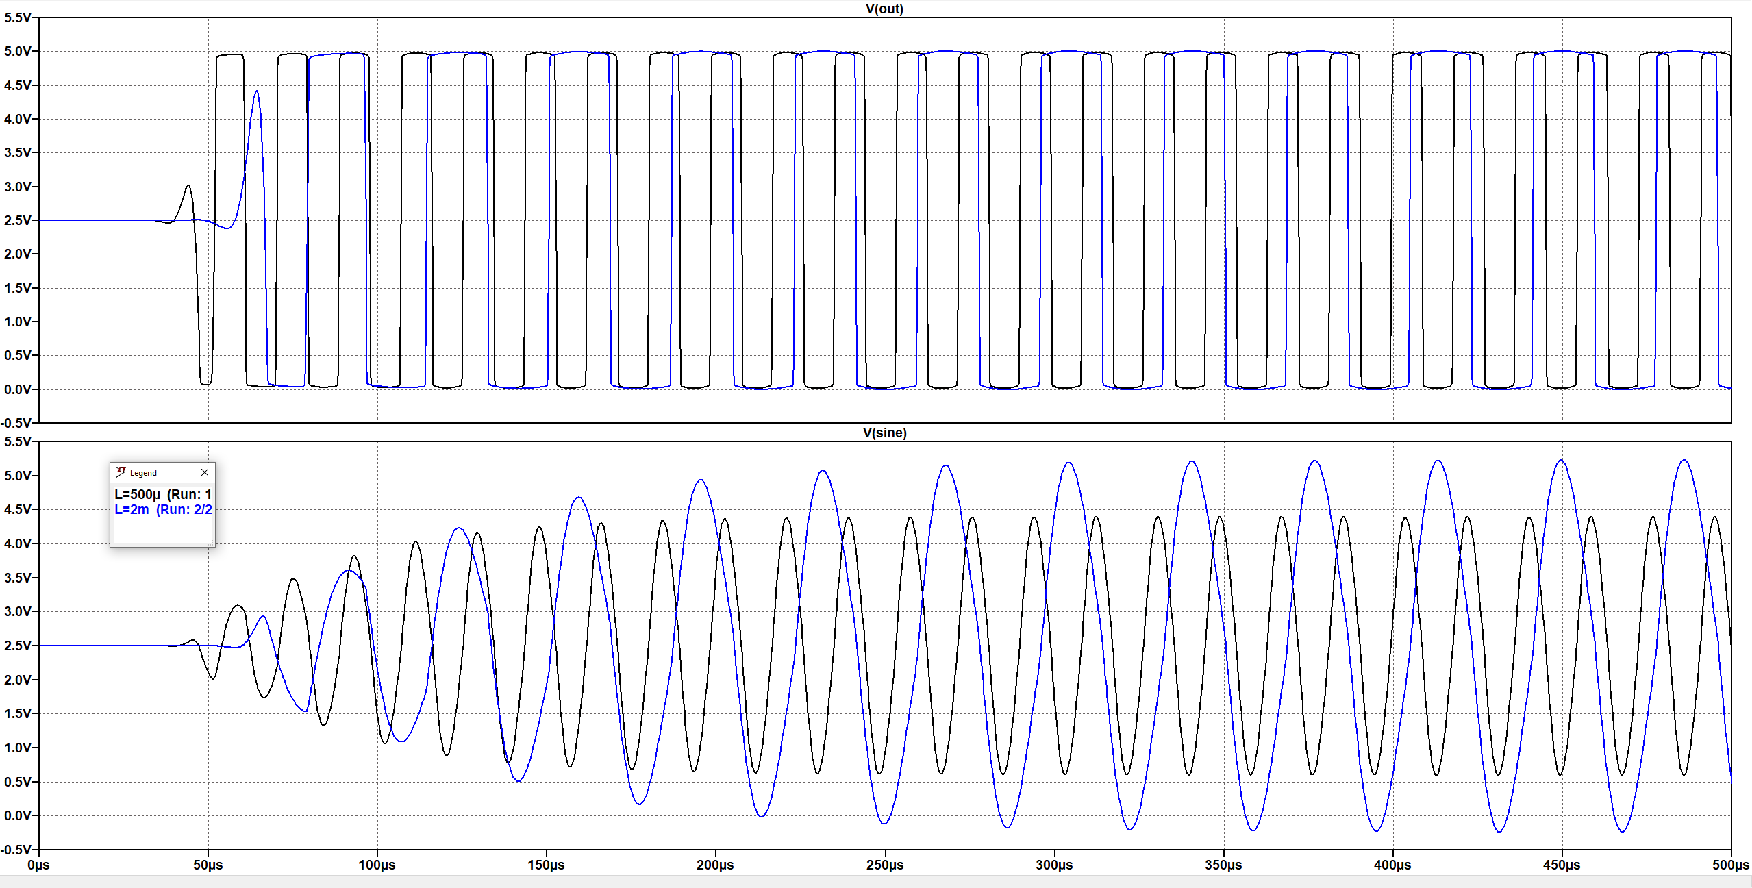
\includegraphics[width=1\linewidth]{fahrzeugerkennung/Colpitts_active_ZB.pdf}
    \caption{Zeitsignale Colpitts-Oszillator}
\end{figure}

Es ist ersichtlich, dass eine Zunahme der Induktivität zu einer Abnahme in der Frequenz der beiden Signale führt.
\pagebreak
\subsection{RS485 Bussystem}
\subsubsection{Benutzte Standards}
\paragraph{ASCII}\mbox{}

ASCII ist eine amerkanischer Standard zur Kodierung einer 7 Bit langen Zeichenfolge. Dieser Standard ermöglicht es Zeichen wie 'A' oder 'b' sowie auch Zahlen und gewissen Sonderzeichen in Bits umzusetzen. 
\paragraph{USB}\mbox{}

Unter USB versteht man eine serielles Bussystem, welches dazu dient Peripherie Geräte mit einem Computer zu verbinden. USB ermöglicht es Geräte während der Laufzeit des Betriebsssystems anzustecken und wieder zu entfernen.
Je nach Version des USB Standards ist es möglich unterschiedliche Datenraten und Leistungen zu verwenden, wobei neuere Standards rückkompatibel zu alten Versionen sind. Für die Ansteuerung des Bussystems ist es notwendig einen Comupter anzuschließen. 
Der USB Standard bietet sich hier an, da er weit verbreitet ist und daher mit vielen Computern kompatibel ist.


\paragraph{UART}\mbox{}


Unter UART versteht man eine eine asynchrone serielle Schnittstelle. Die elektrische Schnittstelle braucht daher auch keine Taktleitung die dem Empfänger der Daten mitteilt wann er zu lesen hat. Stattdessen gibt es zwei Datenleitungen nämlich eine 
für das Senden TX und eine für das Lesen RX. Auf diesen Datenleitungen befinden sich nur die Bitströme des Empfängers und des Senders. Sie besitzen einen Ruhepegel von logisch 1.
UART synchronisiert sich indem es beim Start der Daten ein Startbit schickt, welche Sender und Empfänger synchronisiert. 
Diese beiden Geräte brauchen daher auch genaue interne Uhren, um sich über den Zeitraum des Datenaustausches synchron zu halten.
Die Dauer diese Datenaustausches hängt vor allem von der Bitrate auch genannt Baudrate ab aber auch die Konfiguration der Anzahl von Datenbits und Paritätsbits haben Einfluss auf diese Größe. 
\\
In der folgenden Abbildung ist der zeitliche Verlauf einer Datenleitung dargestellt es wird das Zeichen 'A' in ASCII codiert übertragen bei einer Baudrate von 57600 Zeichen pro Sekunde.

\begin{figure}[H]
    \centering
    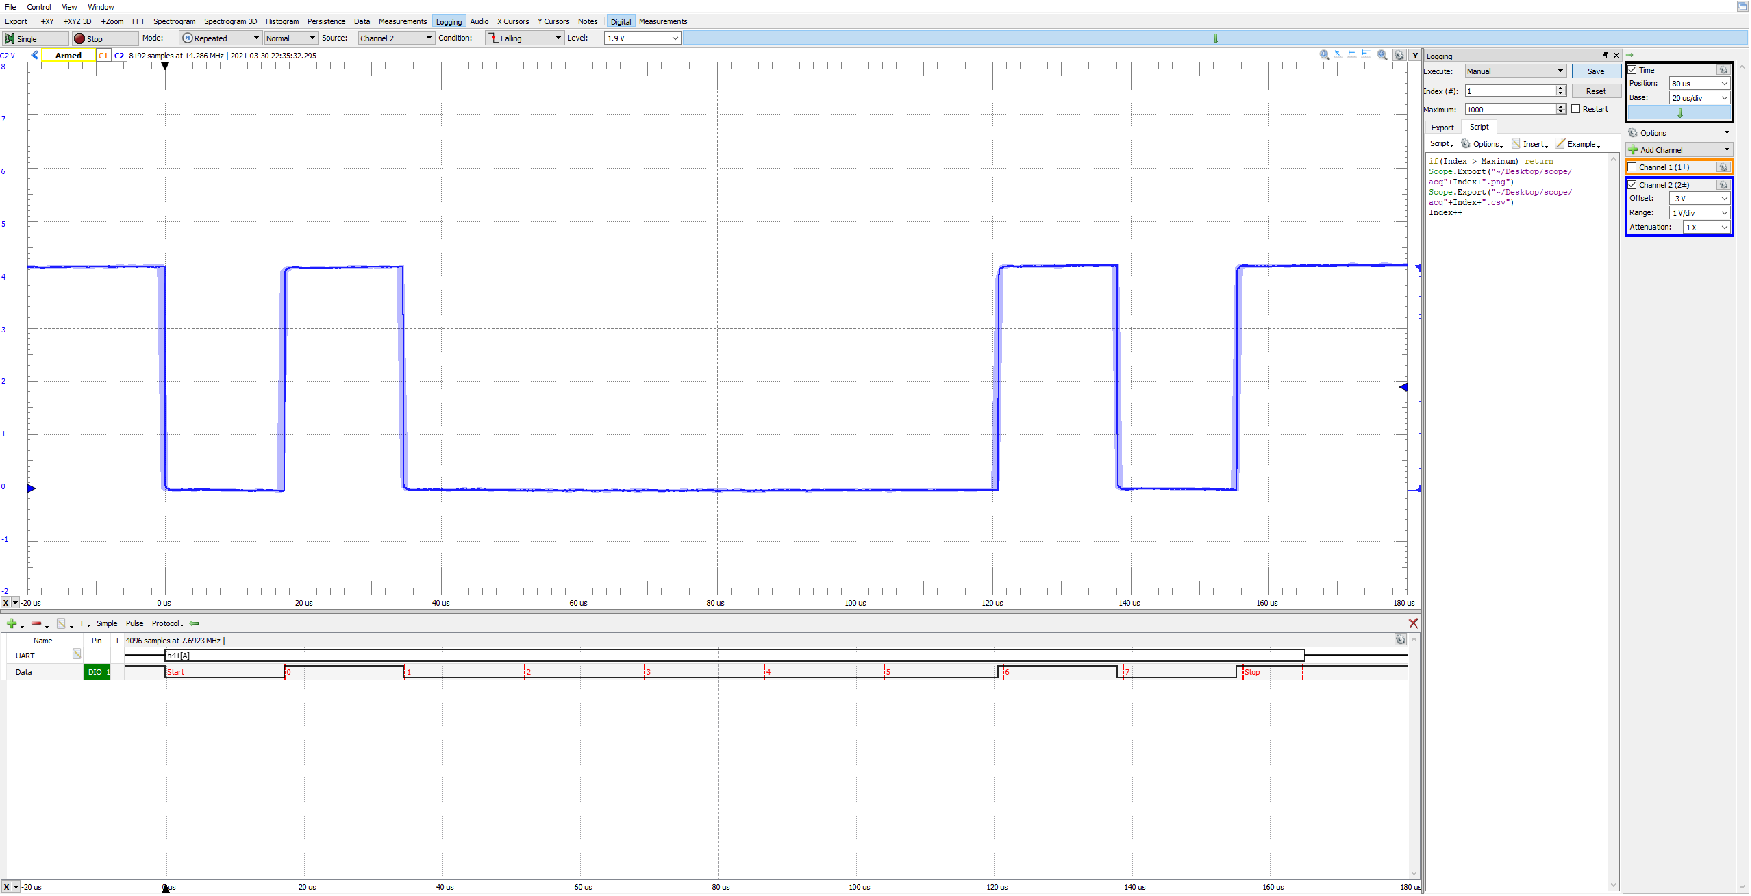
\includegraphics[width=1\linewidth]{fahrzeugerkennung/UART_example.pdf}
    \caption{Beispiel einer UART Zeichenübertragung}
\end{figure}

\paragraph{RS485}\label{sec:RS485}\mbox{}

RS485 ist ein Standard für eine physikalische Schnittstelle für Datenübertragung von UART Daten. Er besitzt zwei symmetrische Leitungen oft mit A und B bezeichnet, dessen Differenzspannung für die Auswertung
des Datenstromes herangezogen wird. Die Verwendung dieser Differenzsignale macht die Schnittstelle sehr robust und industrietauglich.
Er ist dafür ausgelegt mehrere Geräte an die gleiche Leitungen anzuschließen. Die maximale Anzahl an Geräten ist mit 32 fix vorgegeben. Es ist zusätzlich notwendig die Spannungen 
$U_{A}$ und $U_{B}$ im Ruhezustand über einen IC oder einen Spannungsteiler auf fixe Potentiale zu legen. Der Spannungsteiler muss wie folgt aussehen um dem Standard zu entsprechen.

\begin{figure}[H]
    \centering
    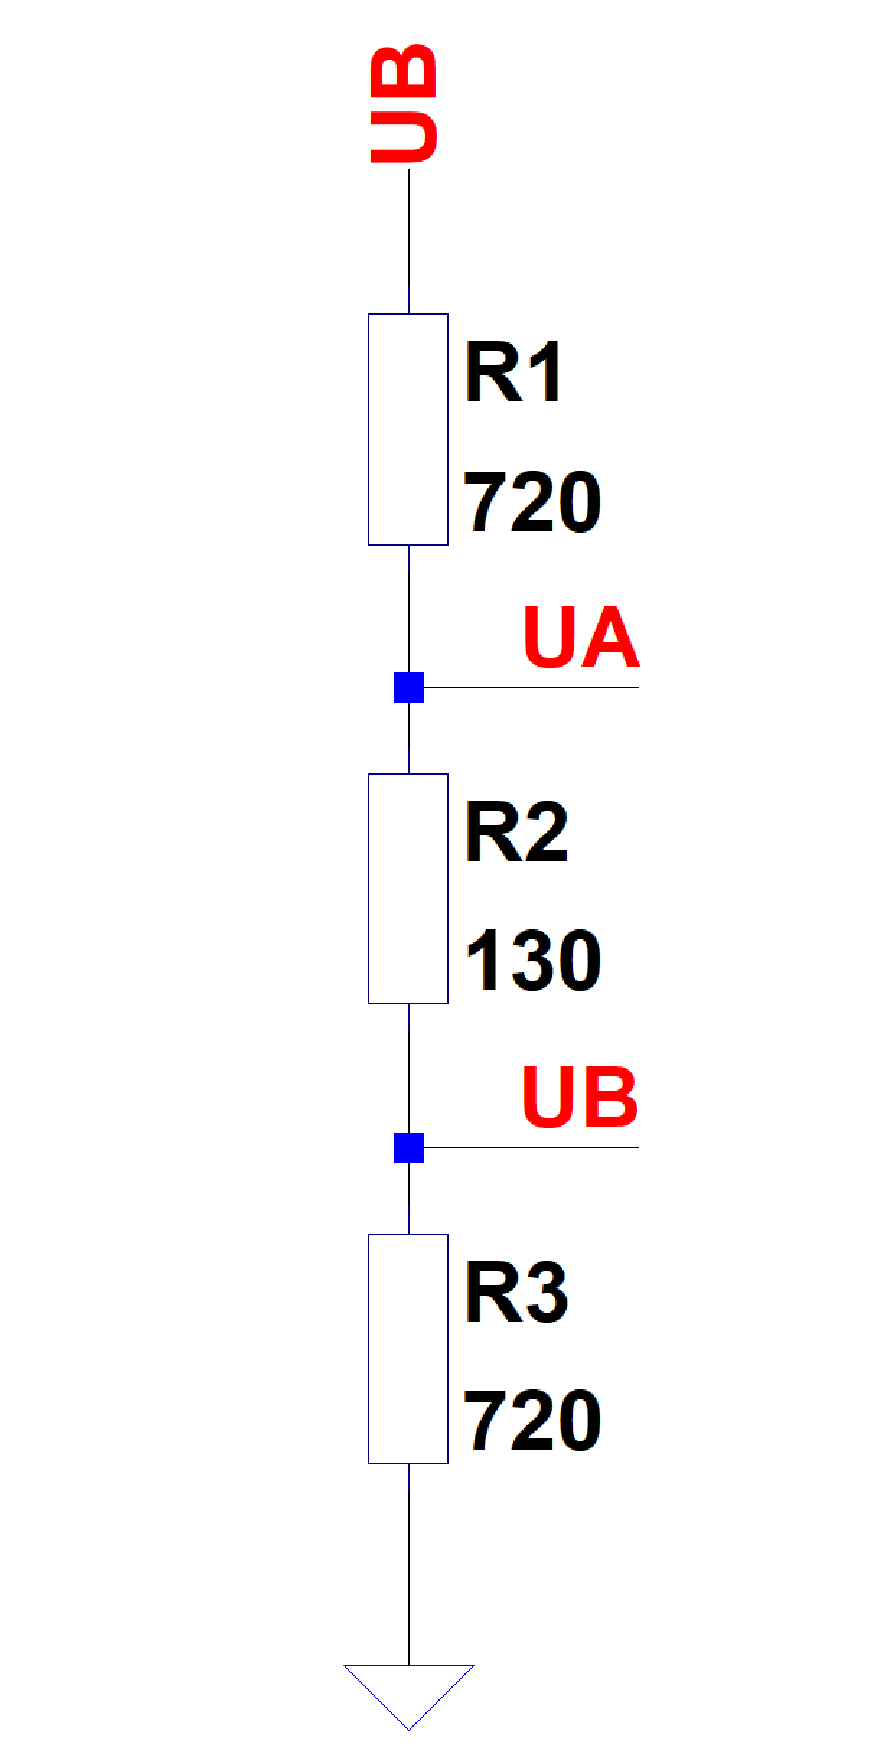
\includegraphics[width=0.15\linewidth]{fahrzeugerkennung/RS485_bias.pdf}
    \caption{RS485 Widerstandsnetzwerk}
    \label{fig:rs485_bias}
\end{figure}

Um diese physikalische Umwandlung zu ermöglichen ist ein Umwandlungs-IC erforderlich. In dieser Arbeit wurde ausschließlich der MAX485CSA für Wandlungen zwischen den Standardpegeln der UART
und die der RS485 Schnittstelle verwendet.

Dieser IC ist busfähig und kann daher seine Ausgänge hochohmig schalten. Er besitzt folgende Eingänge und Ausgänge:
\begin{itemize}
    \item \textbf{!RE: Read enable} \\
    Wenn dieser Eingang auf logisch 0 gesetzt ist wertet der IC das Differenzsignal $U_{AB}$ aus und liefert das Ergebnis an den Ausgang RO.
    Ansonsten setzt er den Ausgang RO in den Tristate beziehungsweise auf hochohmig.
    \item \textbf{DE: Data enable} \\
    Wenn dieser Eingang auf logisch 1 gesetzt ist wird die Spannung am Eingang DI in die zugehörigen Pegel $U_{A}$ und $U_{B}$ umgewandelt.
    Ansonsten setzt er den Eingang DI in den Tristate beziehungsweise auf hochohmig.
    \item \textbf{RO: Read out} \\
    Ist die eingelesene Spannung, die sich logisch aus der Differenzspannung $U_{AB}$ ergibt wenn !RE auf logisch 0 ist.
    \item \textbf{DI: Data In} \\
    Ist die eingehende Spannung, die auf die RS485 Schnittstelle geschrieben werden soll, wenn der Eingang DE auf logisch 1 ist.
\end{itemize}

Die Auswertung der Differenzspannung $U_{AB}$ kann auch in der folgenden Tabelle aus dem Datenblatt des MAX485CSA entnommen werden. 

\begin{figure}[H]
    \centering
    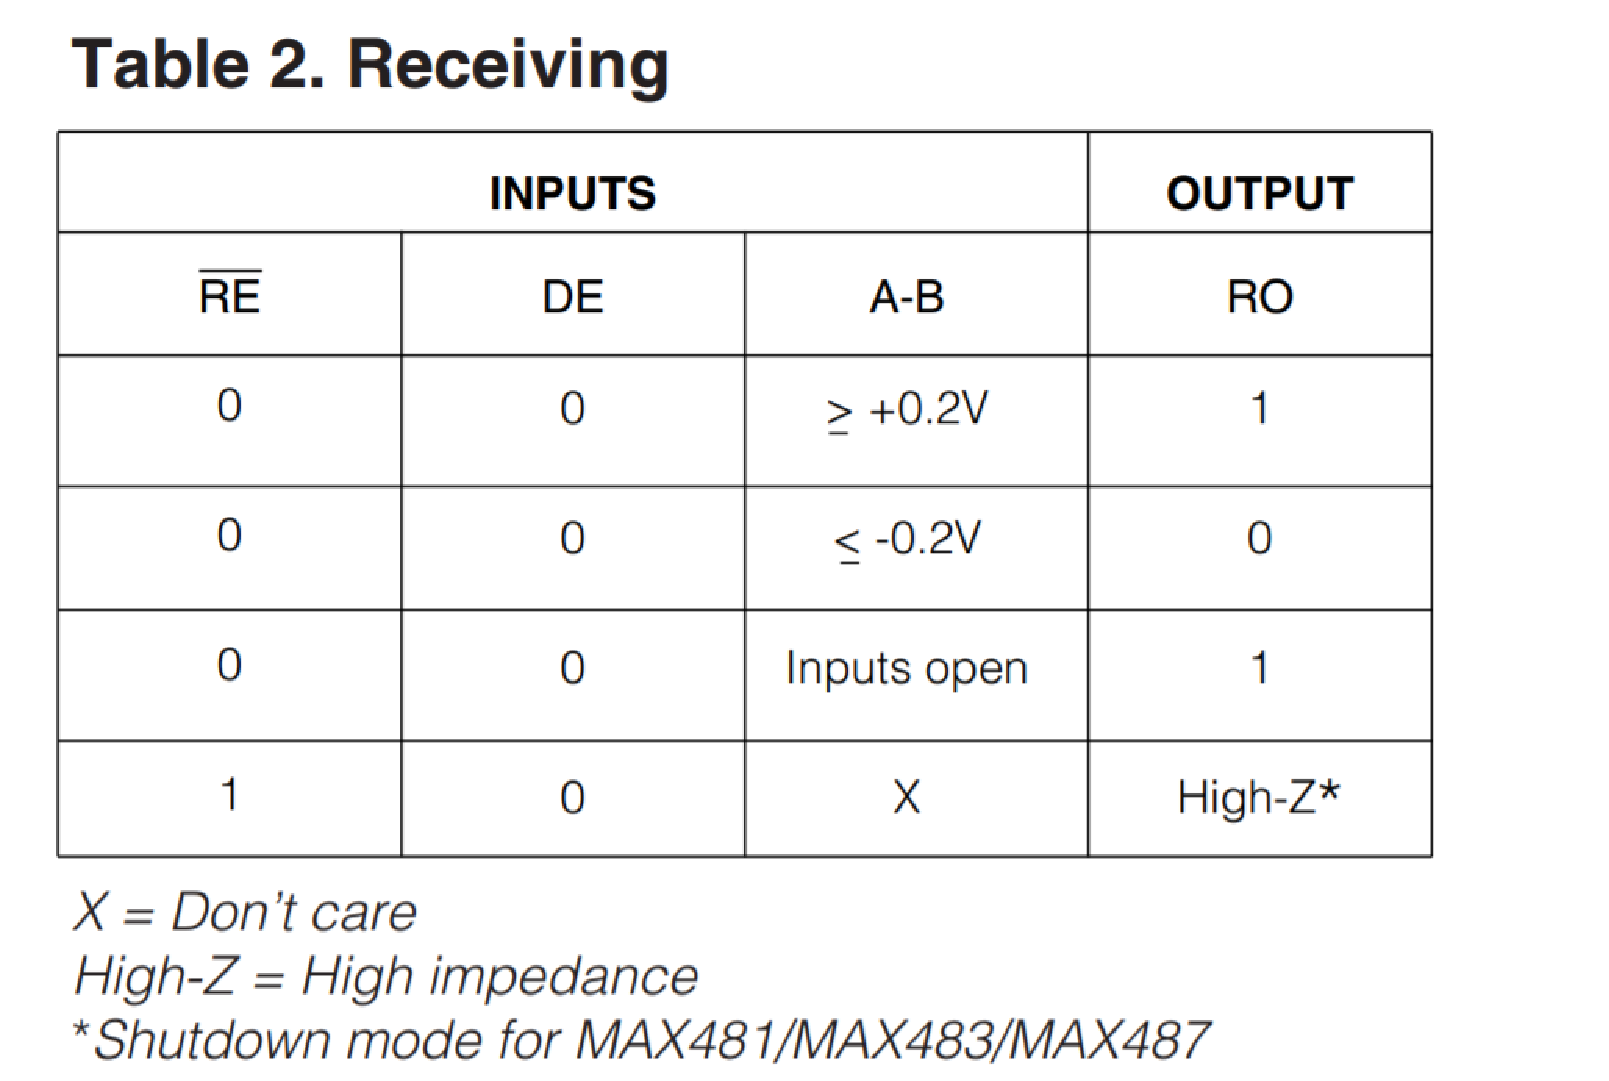
\includegraphics[width=0.6\linewidth]{fahrzeugerkennung/RS485_receiving_table.pdf}
    \caption{Logische Tabelle für $U_{AB}$}
\end{figure}

In der folgenden Abbildung wird wieder das Zeichen 'A' ASCII kodiert versendet nur dieses mal wird eine RS485 Schnittstelle mit den entsprechenden Pegeln verwendet.
In Blau ist die Spannung $U_{A}$ und in Orange die Spannung $U_{B}$ zu sehen. Darunter befindet sich das logische UART Signal am Ausgang RO. 

\begin{figure}[H]
    \centering
    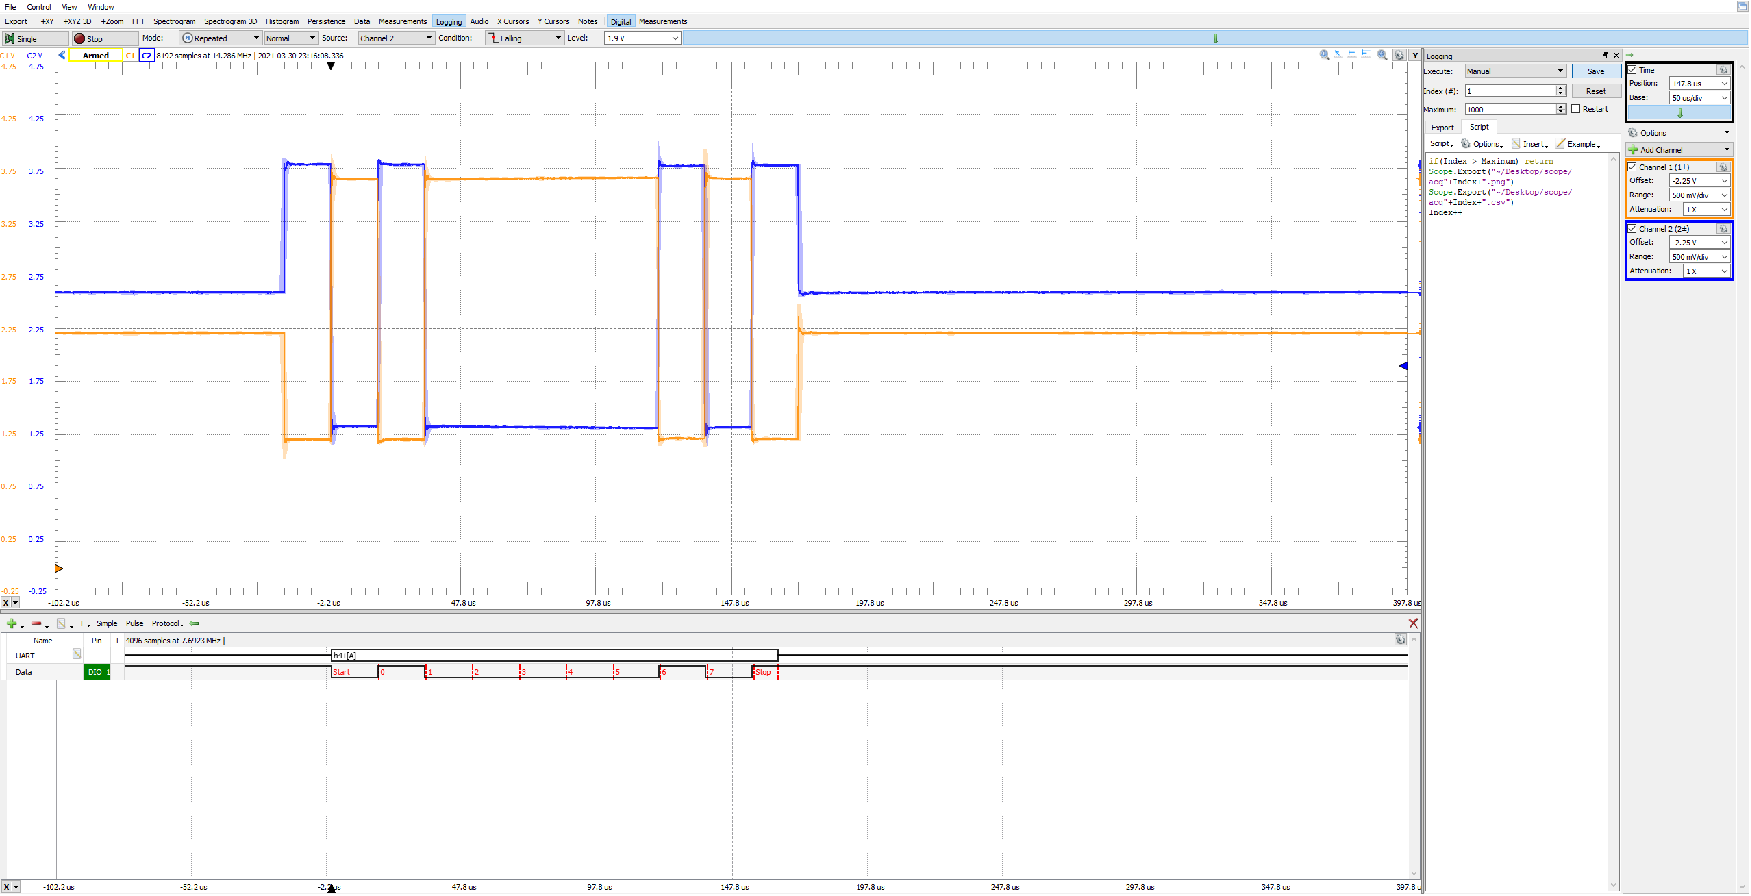
\includegraphics[width=1\linewidth]{fahrzeugerkennung/RS485_example.pdf}
    \caption{Beispiel einer RS485 Zeichenübertragung}
\end{figure}

\paragraph{RJ45}\mbox{}

Um die Anzahl der Kabel zu minimieren und um das Anschließen von Geräten an den Bus einfach zu halten ist ein
mehradriger Stecker mit zugehörigem Kabel nötig.\\
Der 45 Stecker ist ein genormter Stecker und besitzt insgesamt 8 Adern und ist für Kommunikationsanschlüsse gedacht. Er kann daher größere Datenraten zulassen und viele auf dem
Markt vorhandene Kabel haben zusätzliche Abschirmungen, die die Datenleitungen vor elektrischen Störungen schützen. 

\begin{figure}[H]
    \centering
    \includegraphics[width=0.6\linewidth]{fahrzeugerkennung/RJ45_connectors.pdf}
    \caption{RJ45 Steckerbuchse und Kabel}
\end{figure}



\subsubsection{Aufbau}

Das Bussystem wird über eine Master Slave Struktur verwaltet, was heißt, das nur ein einzelnes Master-Gerät andere Teilnehmer am Bus ansprechen kann.
Slave-Geräte können nur nach Anfrage des Masters auf den Bus schreiben. Neben der Steuerung der Kommunikation sollte das Master-Gerät aus praktischen Gründen ebenfalls die Slave-Geräte
mit Energie versorgen und ihnen eindeutige Adressen zuweisen können. \\

In den unteren Abbildungen sind der logische Aufbau und der physikalische Aufbau zu sehen.
Auf die einzelnen Funktionen diverser Leitungen wird in den folgenden Paragraphen eingegangen.

\begin{figure}[H]
    \centering
    \includegraphics[width=1\linewidth]{fahrzeugerkennung/übersicht_bus.pdf}
    \caption{Logische Übersicht des Bussystems}
\end{figure}

\begin{figure}[H]
    \centering
    \includegraphics[width=1\linewidth]{fahrzeugerkennung/übersicht_irl.pdf}
    \caption{Physische Übersicht des Bussystems}
    \label{fig:bus_physical_overview}
\end{figure}
Ganz rechts oben in Schwarz ist der Raspberry Pi der hier als Computer dient es kann aber auch ein anderer Computer verwendet werden. Unterhalb des Raspberry Pi ist der USB-RS485 Wandler der mit einem USB-Kabel
am Raspberry Pi angeschlossen ist und an einer Versorgungsspannung hängt. Der USB-RS485 Wandler ist wiederum mit einem RJ45-Kabel an einen Slave verbunden. In diesem Bild sind zwei Slaves an das Bussystem angeschlossen worden.
Es können aber bis zu 31 sein. Ganz rechts ist der Leitungsabschluss der in Abbildung \ref{fig:rs485_bias} zu sehen ist.
\\ \\
Die elektrische Belegung der Leitungen ist wie in der folgenden Tabelle festgelegt worden. Mit dieser Belegung ist es möglich die Slave-Geräte an den RS485 Datenbus zu legen,
sie mit Spannung zu versorgen und die Adressvergabe mit einer zusätzlichen Logikleitung zu regeln. 

\begin{table}[h]
    \centering
    \begin{tabular}{|c|c|c|c|}
        \hline
        \textbf{Pinnummer} & \textbf{Farbe} & \textbf{Netz} & \textbf{Beschreibung}                      \\ \hline
        1                  & Orange / weiß  & GND           & Masse                                      \\ \hline
        2                  & Orange         & +5V           & 5 Volt Versorgungsspannung                 \\ \hline
        3                  & Grün / weiß    &               & unbelegt                                   \\ \hline
        4                  & Blau           & A             & RS485 positives Datensignal                \\ \hline
        5                  & Blau / weiß    & B             & RS485 negatives Datensignal                \\ \hline
        6                  & Grün           & VCC           & Positive Versorgungsspannung +9V bis 30V   \\ \hline
        7                  & Braun / weiß   & GND           & Masse                                      \\ \hline
        8                  & Braun          & ADR           & Logiksignal zur Vergabe der Slave Adressen \\ \hline
    \end{tabular}
    \caption{RJ45 allgemeine Pinbelegung}
\end{table}

\paragraph{Funktion der Adresslogikleitung}\label{sec:func_adress_wire}\mbox{}

Da alle Teilnehmer des RS485-Busses parallel an den Datenleitungen A und B liegen kann der Master sie voneinander nicht unterscheiden. Dieses Probleme beseitigt die Adressleitung, welche
die einzelnen Geräte logisch aneinanderreiht.

\begin{figure}[H]
    \centering
    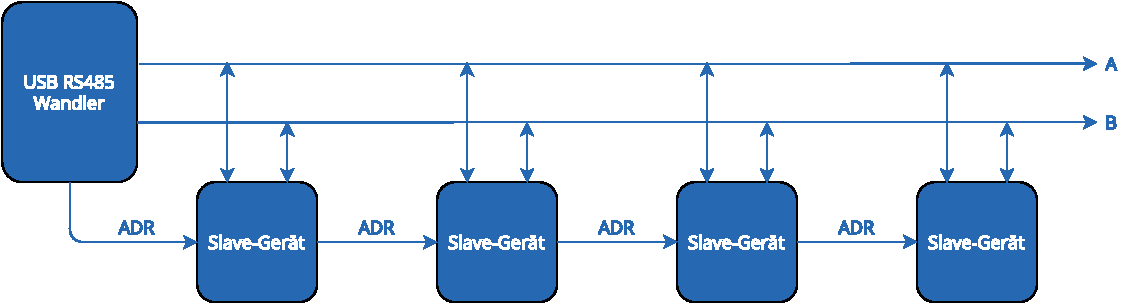
\includegraphics[width=1\linewidth]{fahrzeugerkennung/adress_function.pdf}
    \caption{Anordnung der Slave-Geräte mit Adresslogikleitung}
\end{figure}

Jedes Slave-Gerät setzt seine Adresslogikleitung über einen Pullup-Widerstand auf logisch 1 wenn es keine Adresse zugeordnet bekommen hat.
Als erstes in der Reihe ist der Master, der seine Adresslogikleitung auf logisch 0 setzt und so dem ersten Gerät in der Kette bekannt gibt, dass es eine Adresse zugewiesen bekommt. Wenn es
diese Adresse bekommen hat legt das Slave-Gerät seine ausgehende Adresslogikleitung ADRO auf logisch 0. So kann das nächste Gerät in der Kette erkennen, dass es eine Adresse zugewiesen kriegt, 
indem es auf die eingehende Adressleitung ADRI achtet.\\
In den folgenden Abbildungen sieht man wie die Geräte über den RJ45 Stecker elektrisch am Bus hängen. Der Master hat nur einen Stecker und hat seine Adresslogikleitung fix auf logisch 0 gelegt.
Die Slaves hingegen brauchen zwei Stecker um die Adresskette zu bilden und unterscheiden zwischen eingehender Adresslogikleitung ADRI und ausgehender Adresslogikleitung ADRO. \\
Wenn jedoch die Slaves falsch herum angeschlossen werden und ADRI und ADRO vertauscht sind, kann dieser Fehler vom Mikrocontroller erkannt und behoben werden. Die genauen Details dieser Funktion 
werden in späteren Abschnitten erklärt. 

\begin{figure}[H]
    \centering
    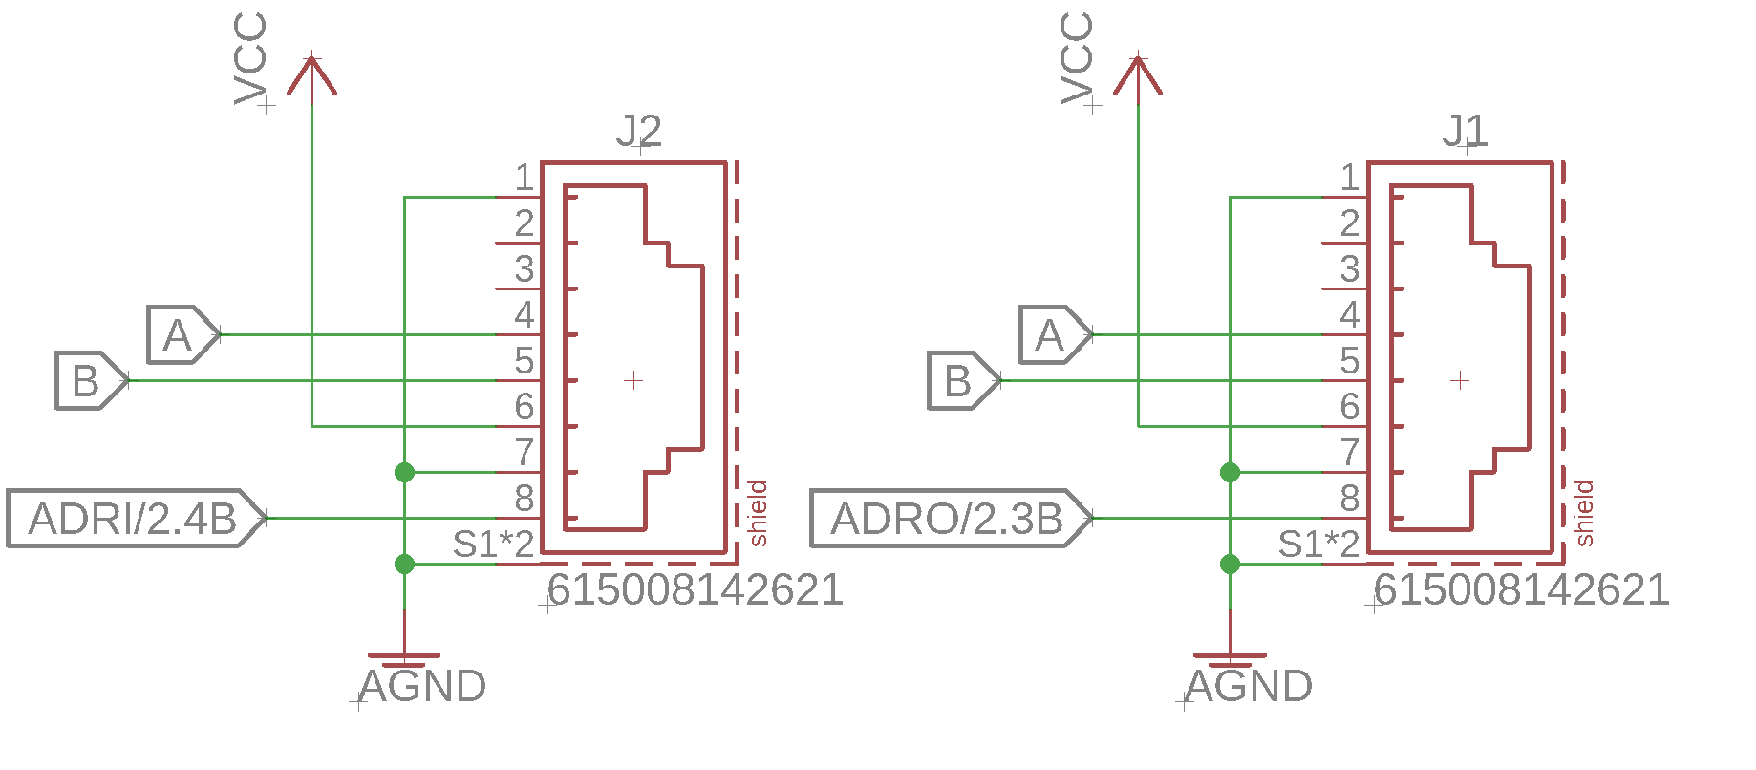
\includegraphics[width=0.6\linewidth]{fahrzeugerkennung/RJ45_slave.pdf}
    \caption{RJ45 Pinbelegung des Slave-Geräts}
\end{figure}

\begin{figure}[H]
    \centering
    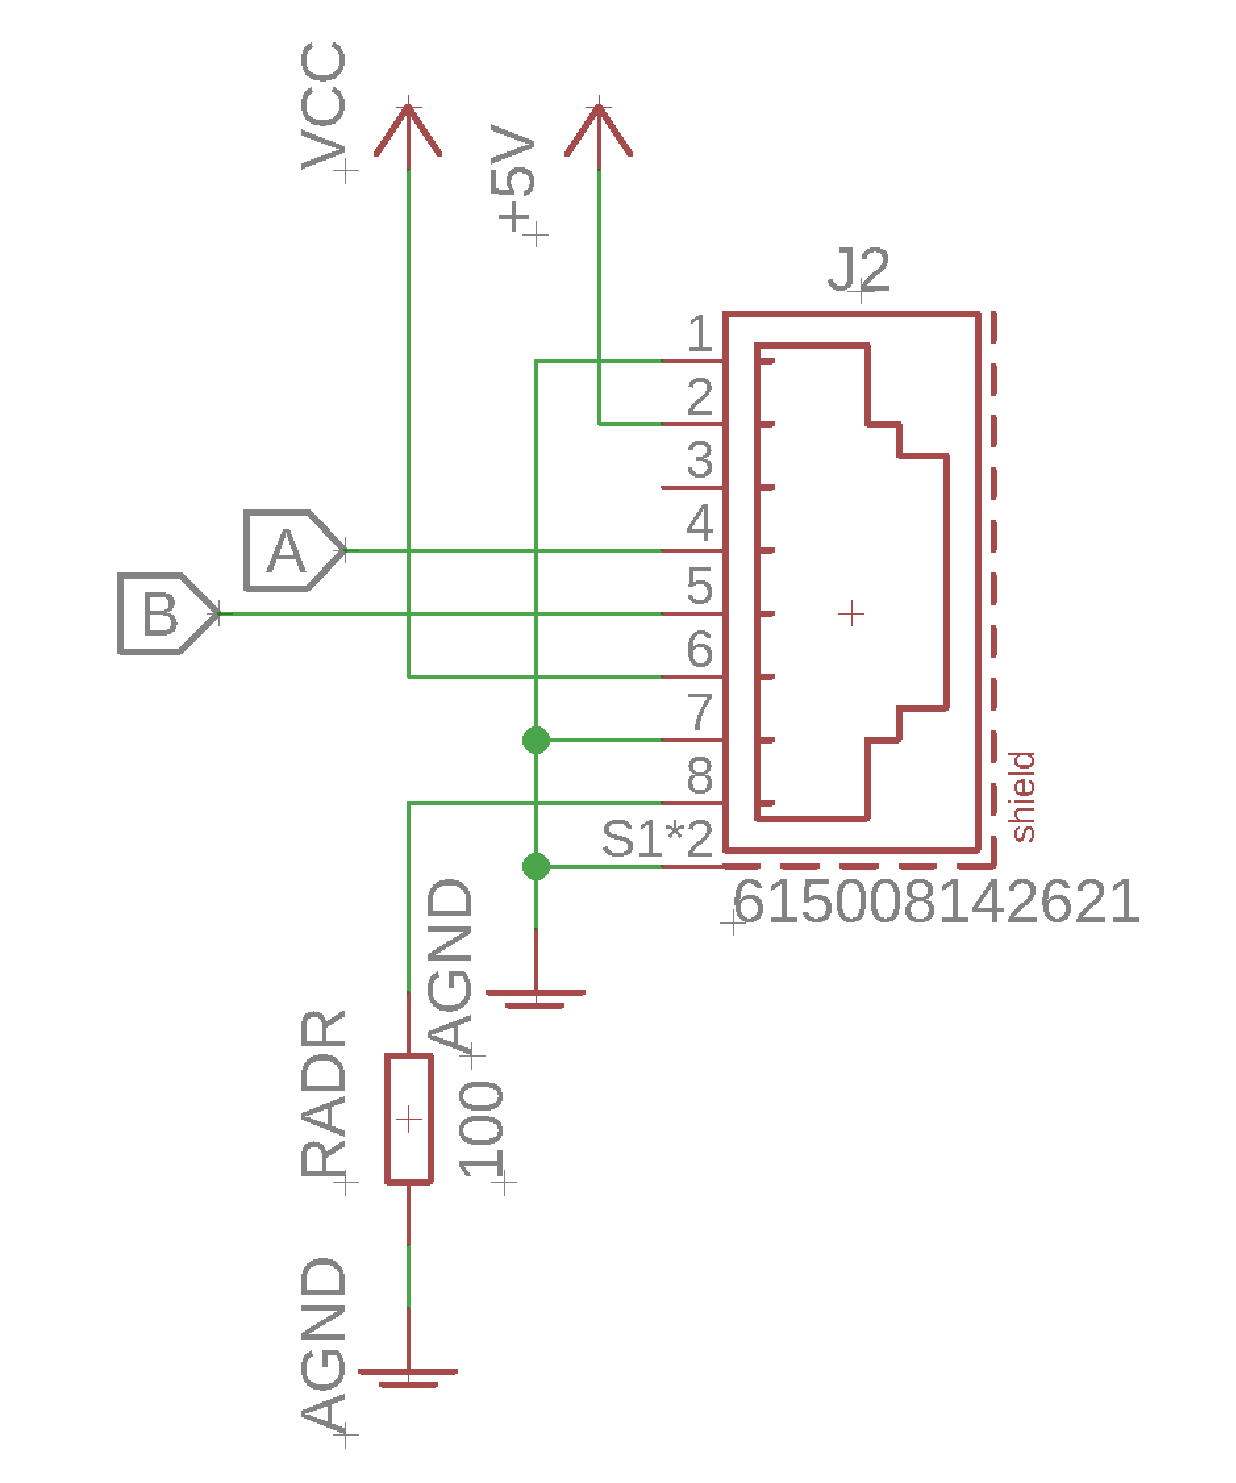
\includegraphics[width=0.3\linewidth]{fahrzeugerkennung/RJ45_master.pdf}
    \caption{RJ45 Pinbelegung des Master-USB-Geräts}
\end{figure}

\paragraph{Versorgungsleitungen VCC und GND}\mbox{}

Da es für jeden Parkplatz ein Slave-Gerät gibt ist die Länge der Busleitung nicht unbeträchtlich. Es kann so entlang der Leitung zu abfallen in der Versorgungsspannung aufgrund des Widerstands der langen Leitungen.
Um dem entgegenzuwirken muss die Versorgungsspannung VCC bezogen auf Masse größer als die benötigte Spannung an den Geräten sein. Die Slave-Geräte besitzen alle einen Linearregler der für eine konstante Spannung von $\SI{5}{\volt}$ sorgt.
Die Eingangsspannung des Spannungsreglers muss je nach Ausführung um eine gewisse Differenzspannung größer sein als die am Ausgang benötigte Spannung. Dieser Wert wird als \textit{Dropout Voltage} bezeichnet. 
Für den IC L78L05ACD lässt sich aus dem Datenblatt folgende Spannung nachlesen: $\SI{2}{\volt}$

\begin{figure}[H]
    \centering
    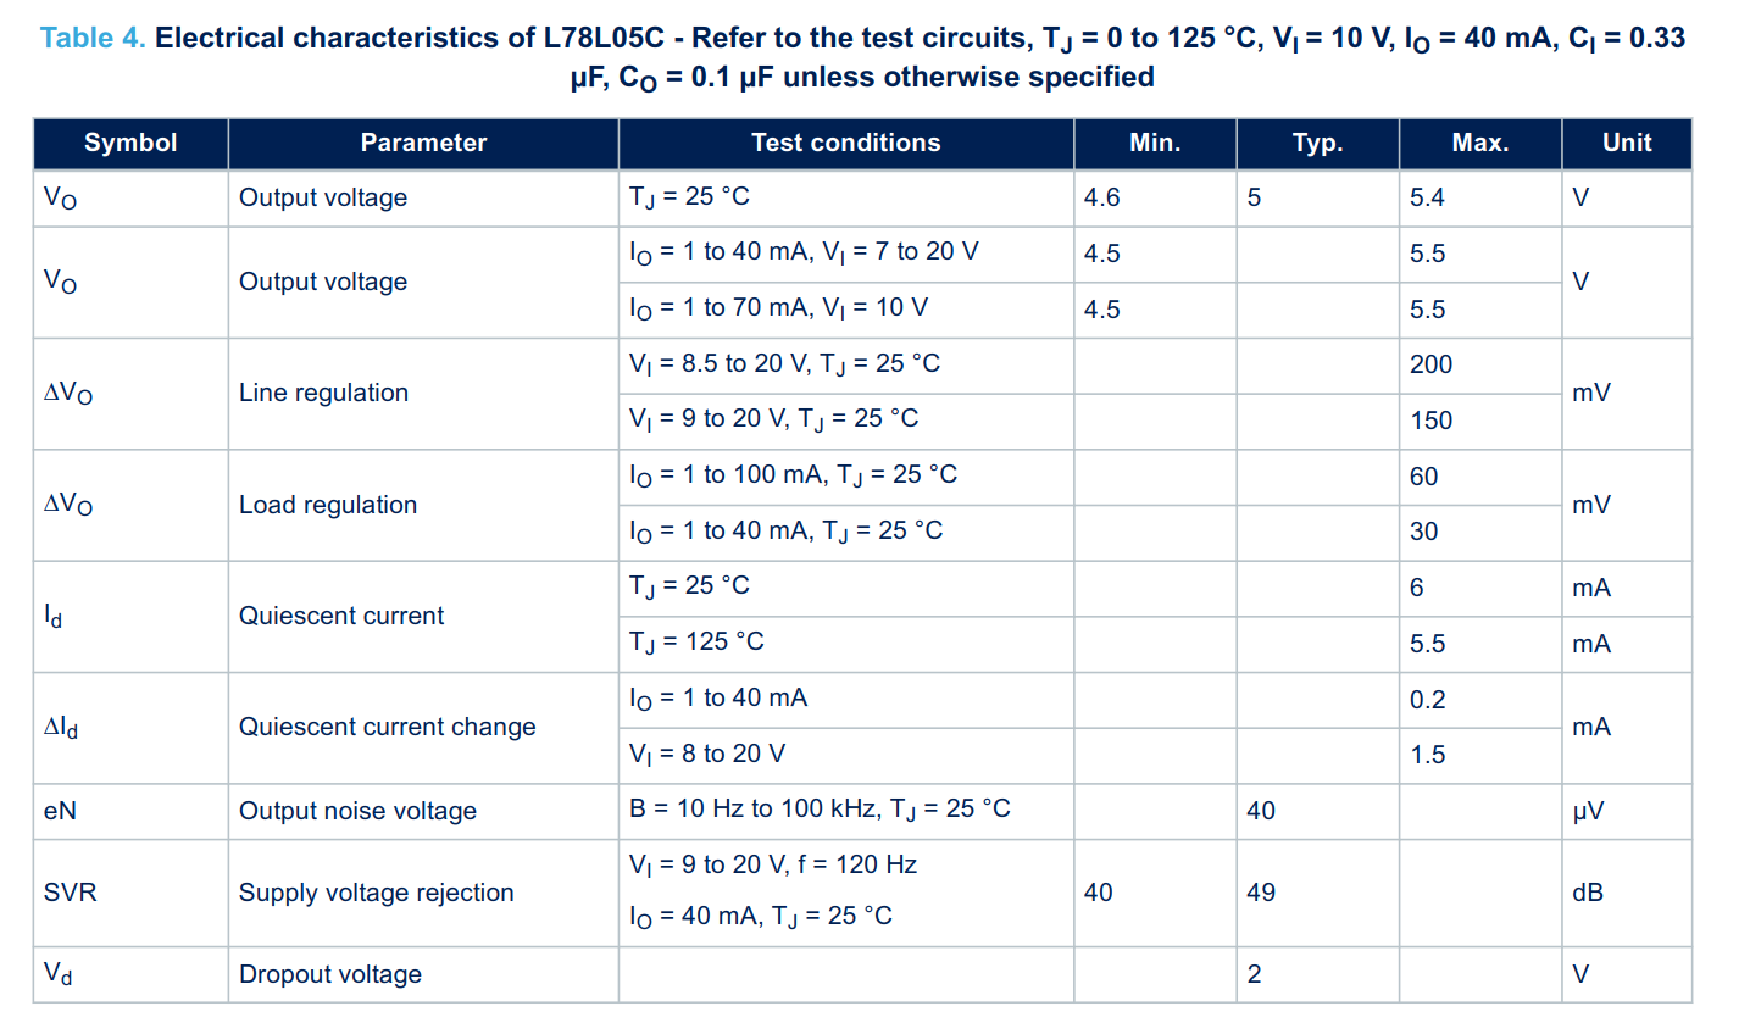
\includegraphics[width=1\linewidth]{fahrzeugerkennung/L78L05_characteristics.pdf}
    \caption{Elektrische Eigenschaften des L78L05ACD}
\end{figure}

Daraus lasst sich schließen dass der IC mindestens eine Spannung von $\SI{7}{\volt}$ braucht um zu funktionieren. Als Eingangsspannung für alle Messung wurde $\SI{9}{\volt}$ verwendet. Nach Datenblatt ist die Eingangsspannung auf 
einen Maximalwert von $\SI{30}{\volt}$ beschränkt. Es ist zu beachten, dass eine Erhöhung der Eingangsspannung zu mehr Verlusten am Linearregler führt und somit für eine schlechte Effizienz sorgt.

\subsubsection{Implementation eines eigenen Protokolls}

RS485 spezifiziert kein Protokoll unter welchem Busteilnehmer untereinander kommunizieren. Es gibt bereits viele fertige Lösung wie zum Beispiel Modbus\footnote{\url{https://www.kunbus.de/modbus.html}}, 
welches auf einer Master/Slave-Architektur basiert. Es ist aber auch möglich ein eigenes Protokoll zu erstellen.
In den folgenden Absätzen wird der Aufbau und die Funktion eines eigen implementierten Protokoll, für die Fahrzeugerkennung, erklärt.
\pagebreak
\paragraph{Aufbau von Datenframes}\mbox{}

Mit UART ist es möglich, unter der Konfiguration von 8 Datenbits, eine Byte pro Datenaustausch zu senden. Diese Bytes bilden die Grundbausteine unseres sogenannten Datenframes, welcher eine Aneinanderreihung von Bytes ist. Jedes Byte
kann eine unterschiedliche Funktion haben. Es kann zum einen einfache Daten beinhalten oder dem anderen Teilnehmer bestimmte Steueranfragen mitteilen. Die Datenframes sind in folgende Grundstruktur aufgeteilt.

\begin{table}[h]
    \centering
    \begin{tabular}{|c|c|c|c|c|c|c|c|c|c|c|c|c|c|c|c|c|}
    \hline
    \multicolumn{17}{|c|}{\textbf{Datenframe}}                                                                                                             \\ \hline
    \textbf{Byte}     & 0     & 1           & 2          & 3    & 4           & 5          & 6  & 7  & 8  & 9  & 10  & 11  & 12  & 13 & 14   & 15   \\ \hline
    \textbf{Name}            & START & \multicolumn{2}{c|}{ADR} & CTRL & \multicolumn{2}{c|}{ARG} & \multicolumn{8}{c|}{DATA\_0 bis DATA\_7} & STOP & LF   \\ \hline
    \textbf{Hexwert}    	 & 0x02  &             &            &      &             &            & \multicolumn{8}{c|}{}                    & 0x03 & 0x11 \\ \hline
    \end{tabular}
    \caption{allgemeiner Aufbau eines Datenframes}
\end{table}

\begin{itemize}
    \item \textbf{START, STOP und LF} \\
    Diese Bytes helfen den Geräten den Anfang und das Ende eines Frames zu erkennen. Das START-Byte signalisiert den Anfang des Datenframes und hat einen fixen Wert von \texttt{0x02} während das Byte STOP mit dem 
    fixen Hexwert von \texttt{0x03} das Ende das Ende signalisiert. Zusätzlich kommt am Ende noch das LF-Byte mit einem Hexwert von \texttt{0x11}. In ASCII kodiert ist das das Zeichen einer neue Zeile in einem Text und ist vorallem nützlich, da
    viele Bibliotheken dieses Zeichen als Endzeichen zu Datenauslesung aus einem seriellen Buffer verwenden.
    \item \textbf{ADR} \\
    Jedes Gerät am Bus ist unter seiner eigenen Adresse erreichbar welche aus zwei Bytes besteht. Die Adressen werden über den Master verteilt, der eine fixe Adresse von \texttt{0x01} besitzt. 
    Zusätzlich sind alle Slaves unter einer Broadcastadresse von \texttt{0x00} erreichbar. Es ergibt sich mit zwei Bytes einen Adressraum der Größe $2^{16} = 65536$ inklusive Master und Broadcast.
    \item \textbf{CTRL} \\
    Das Kontrollbyte CTRL signalisiert einen bestimmten Steuerbefehl. Mit ihm kann man eine Frequenzmessung der Spule an einem Slave auslösen oder einzelne LEDs ein- und ausschalten.
    
    \item \textbf{ARG} \\
    Die Argumentbytes ARG1 und ARG2 geben dem Steuerbefehl zusätzliche Daten mit. 
    So kann man zum Beispiel zwischen LED1 und LED0 und einschalten und ausschalten unterscheiden. 
    
    \item \textbf{DATA} \\
    Das Segment DATA besteht aus 8 Datenbytes, die für den Austausch von größeren Werten, wie einer Frequenz von nutzen sind. Diese Datenbytes sind in ASCII kodiert um Konflikte mit den START, STOP und LF Bytes zu vermeiden. Jedes Datenbyte kann daher einen Hexwert von \texttt{0x0} bis 
    \texttt{0xF} haben. Der größtmögliche Wert, der sich verschicken lässt ist daher \texttt{0xFFFFFFFF} was in Dezimal einem Wert von $2^{32} - 1 = 4 294 967 294$ entspricht.
\end{itemize}

\paragraph{Steuerabläufe}\mbox{}

Um eine Aktion auszuführen schreibt der Master auf den Bus ein Datenframe und wartet auf die Antwort des angesprochenen Slaves. 

\begin{figure}[H]
    \centering
    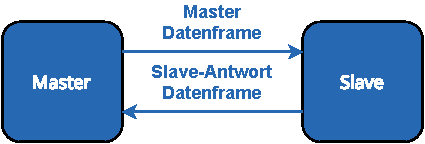
\includegraphics[width=0.4\linewidth]{fahrzeugerkennung/master_slave_dataframes.pdf}
    \caption{Ablauf von Steueranfragen}
\end{figure}

Die Art des Steuerbefehls wird durch das CTRL-Byte angegeben un definiert so die Inhalte der Bytes. Es muss aber zwischen einen Master Datenframe und einem Slave-Response Datenframe unterschieden werden. 
In den nächsten Abbildung werden die möglichen Steuerbefehle für Master und Slave in Tabellenform angeführt.

\begin{sidewaysfigure} 
    \centering
    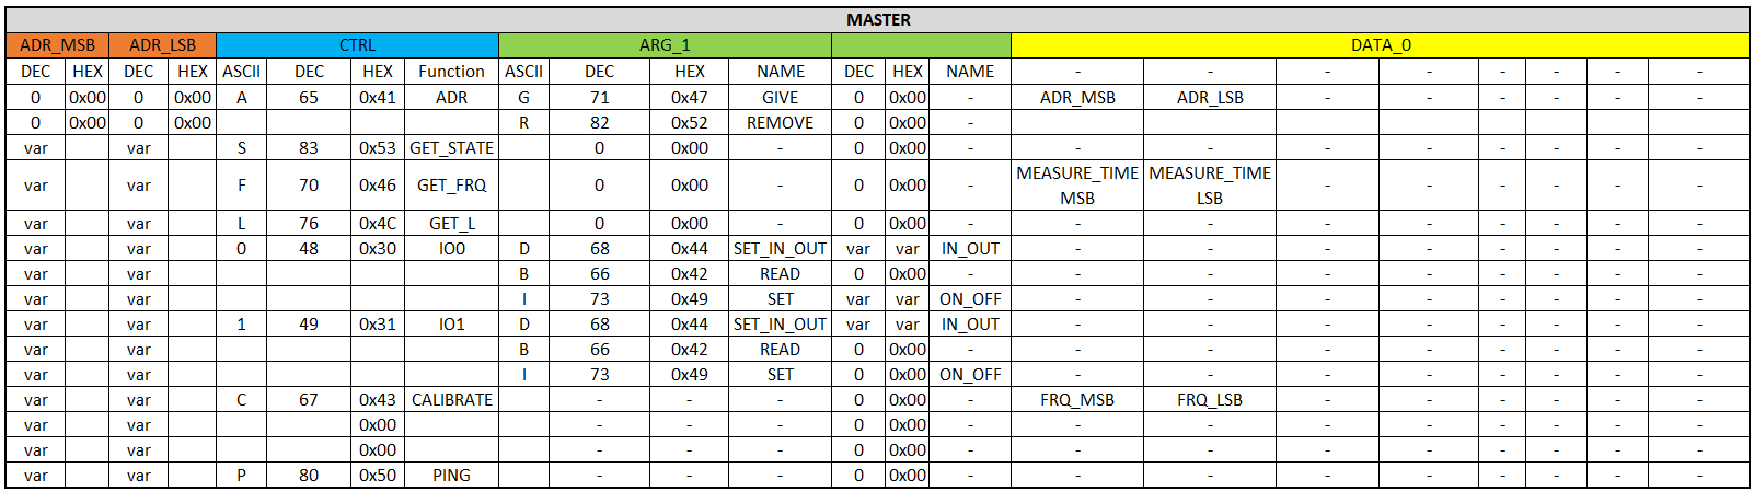
\includegraphics[width=1\linewidth]{fahrzeugerkennung/master_datenframe.pdf}
    \caption{Master Datenframe}
    \label{fig:master_frame}
\end{sidewaysfigure}

\begin{sidewaysfigure}
    \centering
    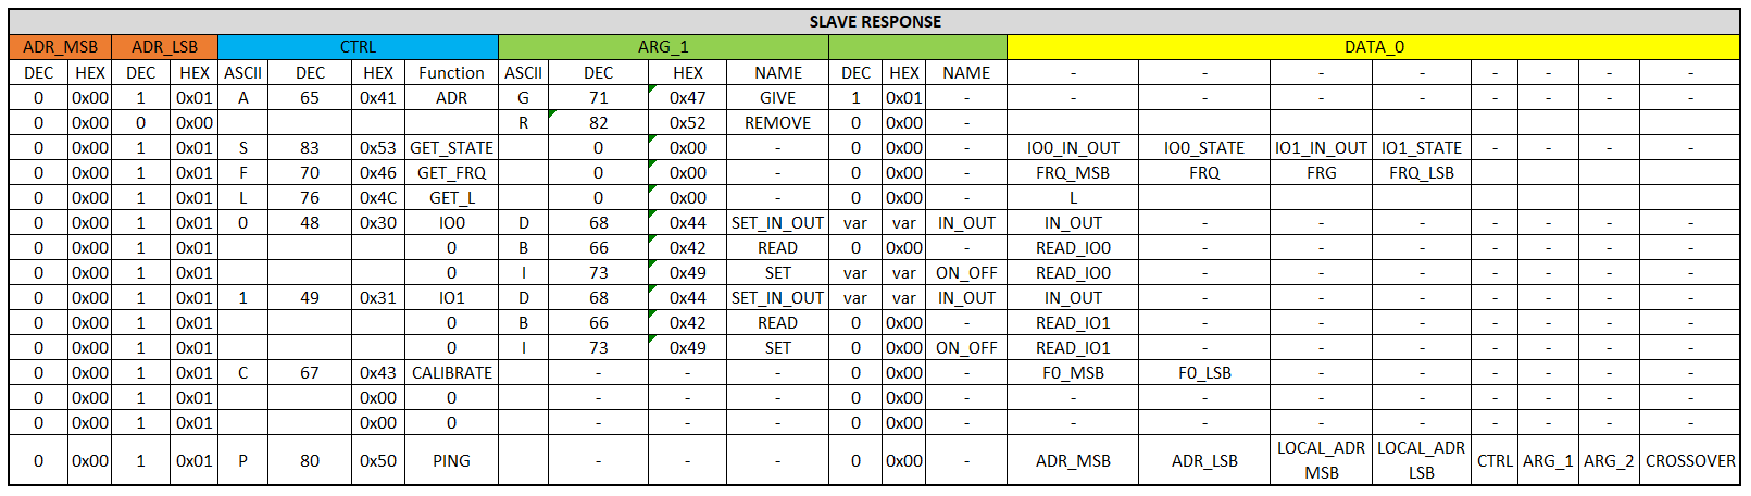
\includegraphics[width=1\linewidth]{fahrzeugerkennung/slave_response_datenframe.pdf}
    \caption{Slave Response Datenframe}
\end{sidewaysfigure}
\pagebreak
Um einen Datenframe beispielhaft darzustellen wird die Anteort des Slaves auf den Befehl IO1 aufgenommen.
Wir erhalten folgendes Bild am Oszilloskop.

\begin{figure}[H]
    \centering
    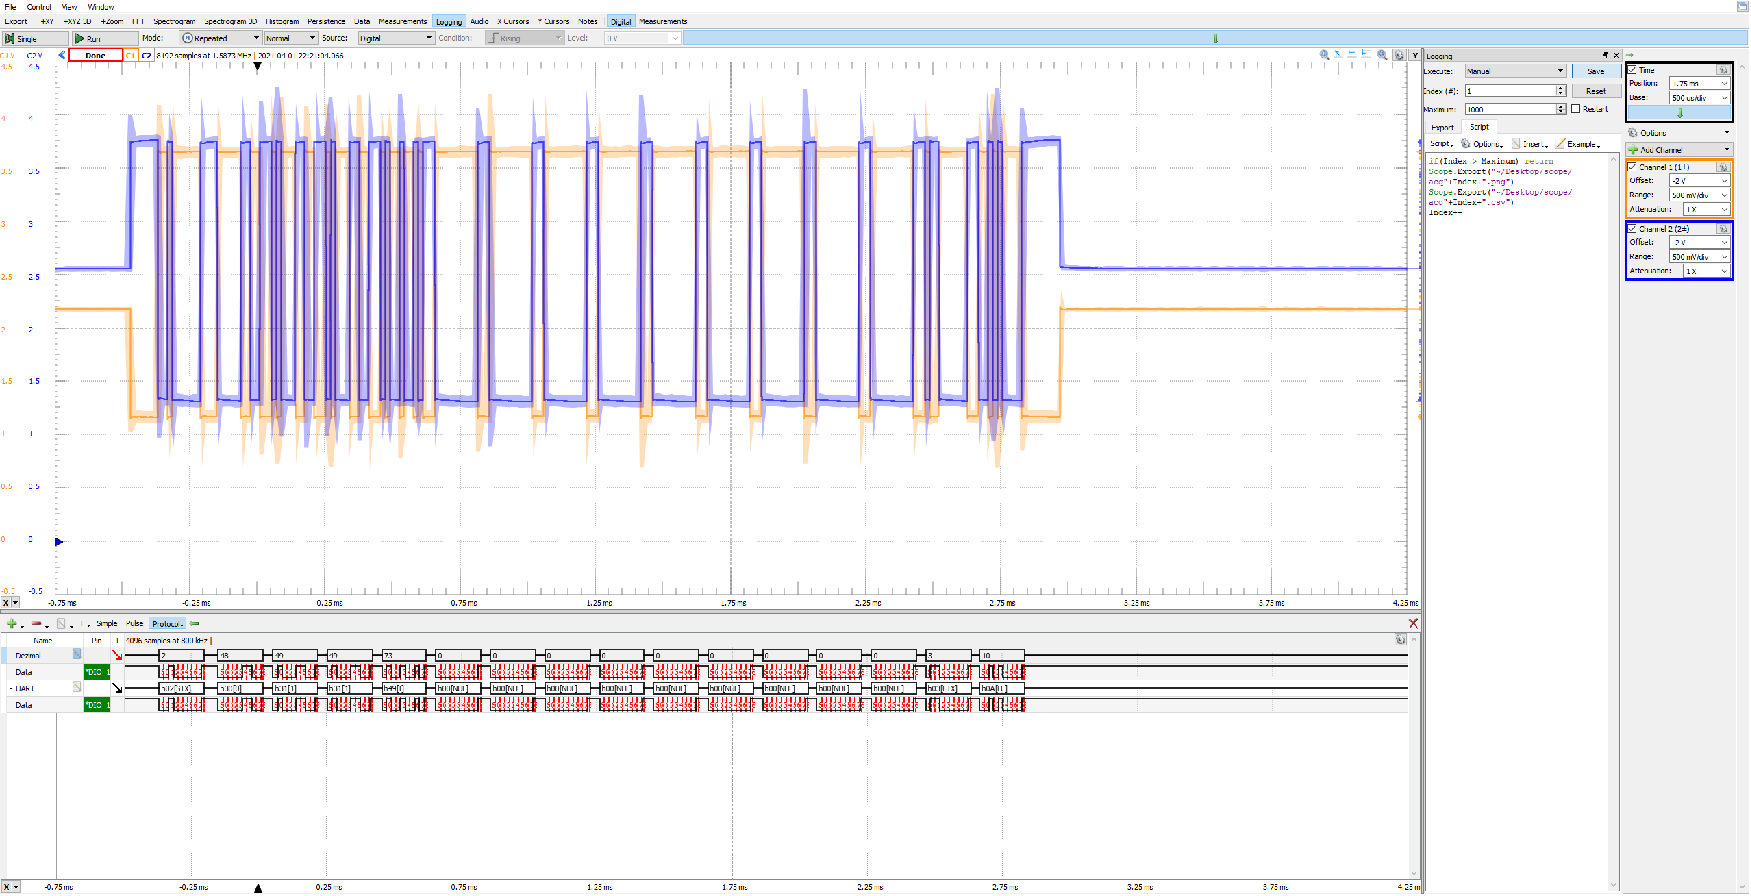
\includegraphics[width=1\linewidth]{fahrzeugerkennung/slave_resp_measured_dataframe.pdf}
    \caption{gemessene Slave Response bei Steuerbefehl IO1}
\end{figure}

\begin{table}[h]
    \centering
    \begin{tabular}{|c|c|c|c|c|c|c|c|c|l|l|l|l|l|l|c|c|}
        \hline
        \multicolumn{17}{|c|}{\textbf{Datenframe}}                                                                                           \\ \hline
        \textbf{Byte}  & 0     & 1           & 2          & 3    & 4           & 5          & 6    & \multicolumn{7}{c|}{7-13} & 14   & 15   \\ \hline
        \textbf{Name}  & START & \multicolumn{2}{c|}{ADR} & CTRL & \multicolumn{2}{c|}{ARG} & \multicolumn{8}{c|}{DATA}        & STOP & LF   \\ \hline
        \textbf{Hex}   & 0x02  & 0x30        & 0x31       & 0x31 & 0x49        & 0x00       & 0x30 & \multicolumn{7}{c|}{0x00} & 0x03 & 0x11 \\ \hline
        \textbf{ASCII} & STX   & 0           & 1          & 1    & I           & NUL        & 0    & \multicolumn{7}{c|}{NUL}  & ETX  & LF   \\ \hline
    \end{tabular}
    \caption{ausgelesene Bytes aus einem gemessenen Datenframe}
\end{table}

Wir sehen dass die Bytes START, STOP und LF die fix zugewiesenen Werte \texttt{0x02, 0x03} und \texttt{0x11} haben. Die ADR Bytes haben ASCII dekodiert die Zeichen '0' und '1' welche zusammengezählt die Adresse 1 ergeben. 
Dies ist die fixe Adresse des Masters und stimmt auch mit unserem Master/Slave System überein, wo die Slaves Datenframes nur an den Master zurück schicken. Das Kontrollbyte CTRL hat den Hexadezimalwert \texttt{0x31} 
und entspricht ASCII dekodiert dem Zeichen '1'. Sieht man nun in der Tabelle mit den Slave-Response Datenframes nach erhalten wir den Befehl IO1. Mit diesem Befehl wird ein digitaler Ein- und Ausgang des Mikrocontroller gesteuert.
Das erste Argumentbyte ergibt ASCII dekodiert das Zeichen 'I' was laut gleicher Tabelle SET bedeutet. Das zweite Argumentbyte hat den Hexadezimalwert \texttt{0x30} welches dekodiert das ASCII Zeichen '0' ist. Dieses Zeichen gibt an,
dass der Ausgang IO1 auf logisch 0 zu schalten ist. Die Datenbytes für den Befehl IO1 sind bis auf das erste Byte alle von sich aus leer. Das erste Datenbyte soll bestätigen dass der Ausgang auf logisch 0 geschalten worden ist und tatsächlich steht 
diesem Byte das Zeichen '0'.  
\\ \\
Der interne C-Code des Slave generiert für den IO1 Befehl die Antwort auf folgende Weise.
\begin{listing}[H]
    \begin{minted}{c}
    unsigned char response[8] = {0, 0, 0, 0, 0, 0, 0, 0};
    IO1_OUT;
    if(argument_2 == OFF)
    {
        IO1_OFF; 
        response[0] = 0x30;
    }
    else if(argument_2 == ON)
    {
        IO1_ON;
        response[0] = 0x30;
    }
    rs485_write_frame(MASTER_MSB, MASTER_LSB, IO1, SET, NONE, response);
    \end{minted}
    \caption{Response C-Code des Slave für IO1}
  \end{listing}

Das Slave-Gerät setzt IO1 als Ausgang und überprüft das zweite Argumentbyte auf dessen Inhalt und setzt den Ausgang je nachdem auf logisch 1 oder 0.
\pagebreak
\subsection{Mikrocontroller Slave-Gerät}

\begin{figure}[H]
    \centering
    \includegraphics[width=0.6\linewidth]{fahrzeugerkennung/uC_slave_orthagonal.pdf}
    \caption{Slave-Geräte mit Gehäuse}
\end{figure}

\begin{figure}[H]
    \centering
    \includegraphics[width=0.6\linewidth]{fahrzeugerkennung/uC_slave_front.pdf}
    \caption{Slave-Geräte mit Gehäuse von vorne}
    \label{fig:slave_front}
\end{figure}

\subsubsection{Überblick}

In der folgenden Abbildung sind alle wichtigen ICs, Ein- und Ausgänge und deren logische Verknüpfungen dargestellt. 

\begin{figure}[H]
    \centering
    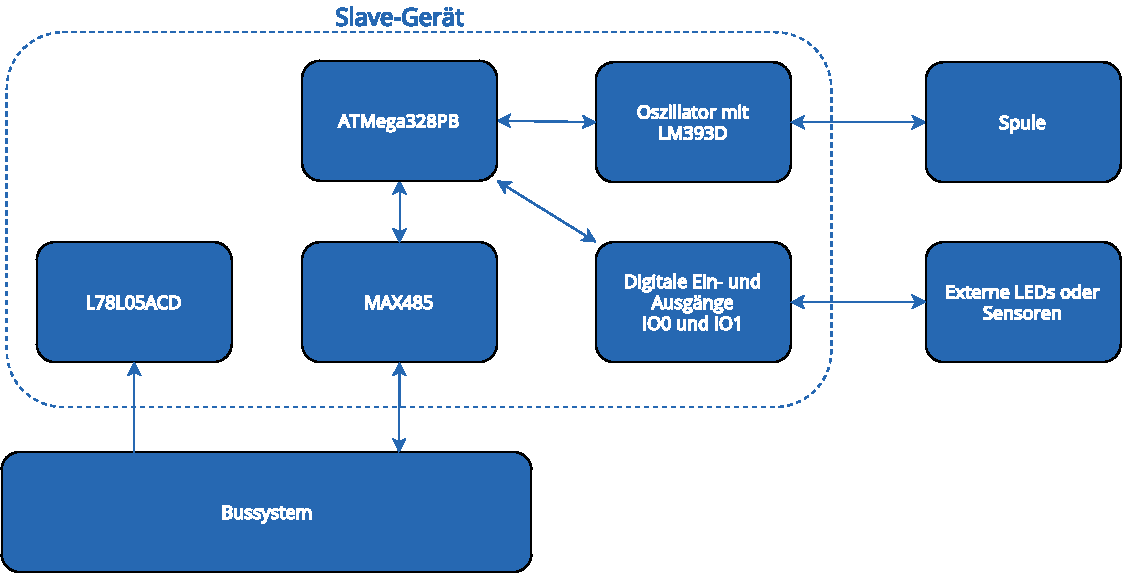
\includegraphics[width=1\linewidth]{fahrzeugerkennung/slave_overview.pdf}
    \caption{Logischer Aufbau des Slave-Gerät}
\end{figure}

\begin{itemize}
    \item \textbf{Atmega328PB} \\
    Ist der Mikrocontroller des Slave-Geräts. Er liest die Frequenz des Oszillator, kontrolliert die Ein- und Ausgänge IO0 und IO1 und ist für die serielle Kommunikation mit dem Bus verantwortlich.
    \item \textbf{L78L05ACD} \\
    Ist ein Spannungsregler, der die erhöhte Spannung aus dem Bussystem absenkt und dem Slave zur Verfügung stellt.
    \item \textbf{MAX485} \\
    Ist ein RS485 Pegelwandler, der die UART Signale des Mikrocontroller in die entsprechenden Pegel umwandelt
    \item \textbf{Oszillator} \\
    An ihn wird die Spule angeschlossen. Er erzeugt mit einer Colpitts-Schaltung eine Resonanzfrequenz die vom Mikrocontroller ausgelesen wird.
    
    \item \textbf{IO0 und IO1} \\
    Es handelt sich um digitale Eingänge und Ausgänge des Mikrocontroller, welche je nach Anwendung unterschiedliche Funktionen haben können. 
    An ihnen hängen zwei LEDs nämlich LED0 und LED1.
\end{itemize}

In den folgenden Absätzen wird genauer auf diese angeführten Blöcke eingegangen.

\subsubsection{Mikrocontroller}

Mikrocontroller\footnote{\url{https://www.mikrocontroller.net/articles/Mikrocontroller}} (auch µC) sind Halbleiterchips die einen integrierten Prozessor, einen Arbeitsspeicher, einen Programmspeicher und eine Peripheriefunktionalität aufweisen. Viele dieser Mikrocontroller besitzen Schnittstellen wie SPI, IIC oder UART
und können analoge Spannung einlesen sowie PWM Signale erzeugen. Ihre vielfältigen Eigenschaften machen diese ICs vielseitig einsetzbar. Sie werden oft in einfachen elektronischen Alltagsgegenständen wie Digitaluhren, Fernbedienungen oder Tastaturen gefunden. 

\begin{figure}[H]
    \centering
    \includegraphics[width=0.4\linewidth]{fahrzeugerkennung/Atmega328PU.pdf}
    \caption{Atmega328PU in DIP28}
\end{figure}

Für die Slave-Geräte ist ein Mikrocontroller sehr gut geeignet, da er keine komplexen Rechnungen durchführen muss. Er soll mit einer seriellen Schnittstelle arbeiten, Rechtecksignale im $\SI{40}{\kilo\hertz}$ bis $\SI{200}{\kilo\hertz}$ Bereich genau bestimmen und
digitale Eingänge und Ausgänge aufweisen können. Auch Interrupts sind vorhanden, welche es möglich machen bei internen oder externen Ereignissen gewissen Programmteile auszuführen.



Der Atmega328PB ist ein Mikrocontroller der Microchip AVR Familie\footnote{\url{https://www.microchip.com/en-us/products/microcontrollers-and-microprocessors/8-bit-mcus/avr-mcus}} und besitzt eine maximale Taktfrequenz von $\SI{20}{\mega\hertz}$ und kann mit einer Betriebsspannung von $\SI{5}{\volt}$ arbeiten.
Sein interner programmierbarer Flash-Speicher ist ist \texttt{32KB} groß, was für diese Anwendung genügend ist.

\subsubsection{Lineare Spannungsregler}

Spannungsregler haben die Aufgabe eine Gleichspannung abzusenken und zu stabilisieren. Sie werden oft bei Schaltungen eingesetzt, bei denen entweder kleine Ströme fließen oder die Effizienz der Schaltung nicht im Vordergrund steht.
Lineare Spannungsregler verwenden Leistungstransistoren um die Spannung abzusenken, was zu Verlustleistungen führt. Die Größe der Ausgangsspannung kann entweder über externe Beschaltung vorgegeben werden oder ist fix vom Hersteller eingestellt. Spannungsregler stellen 
immer automatisch die richtige Ausgangsspannung ein, selbst wenn die Eingangsspannung in einem vorgegebenen Bereich variiert. 
\\ \\

Weil der Mikrocontroller eine Betriebsspannung von $\SI{5}{\volt}$ benötigt ist ein Spannungsregler mit dieser Ausgangsspannung erforderlich. Der L78L05ACD erfüllt diese Eigenschaften und kann 
eine Ausgangsspannung von $\SI{5}{\volt}$ bei einer Eingangsspannung von $\SI{7}{\volt}$ bis $\SI{30}{\volt}$ erzeugen. Der maximalen Strom beträgt $\SI{100}{\milli\ampere}$.

\begin{figure}[H]
    \centering
    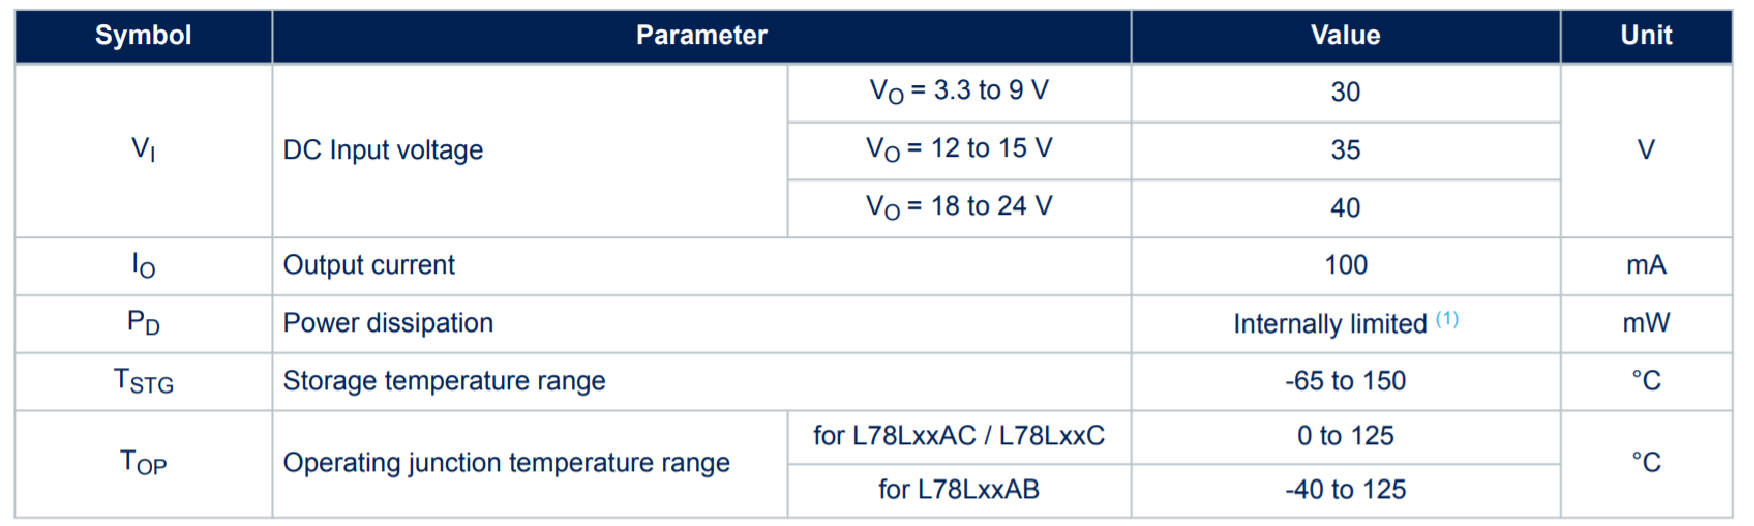
\includegraphics[width=1\linewidth]{fahrzeugerkennung/L78L05_max_ratings.pdf}
    \caption{absolute Grenzwerte des L78L05ACD}
\end{figure}

\subsubsection{RS485 Pegelwandler}

Die Aufgabe des RS485-Pegelwandlers ist die Umsetzung der UART-Spannungspegel in RS485-Spannungspegel. Die Einzelheiten dieses Standards und die wichtigen Funktionen des MAX485CSA 
sind im Absatz \ref{sec:RS485} beschrieben.

\subsubsection{Oszillator mit LM393D Komparator}

Der Oszillator dient dazu die Induktivität der Spule in eine Frequenz umzusetzen (Vergleiche Absatz \ref{sec:colpitts}). Dafür ist ein aktives Element nötig, das für eine Phasendrehung von $\SI{180}{\degree}$ sorgen kann.
Es kann dabei ein Operationsverstäker in Frage kommen aber auch ein einfacher Komparator ist hier ausreichend. Um das Sinussignal des Oszillator in ein Rechtecksignal für den Mikrocontroller umzuwandeln ist ein zusätzlicher Schmitttrigger nötig.
Der Grund dafür ist eine Funktionalität des Mikrocontrollers. Er besitzt nämlich eine Interrupt Funktionalität, die auf Flanken von Rechtecksignalen reagiert. Über die Zählung der Flanken über einen Zeitraum lässt sich die Frequenz ermitteln.
Das Schmitttrigger ist deshalb ausgewählt worden, weil das Eingangssignal einen gewissen Betrag überschreiten, beziehungsweise unterschreiten muss bevor das Ausgangssignal sich ändert. 
Dieser Schwellwert ist bei einer Betriebsspannung von $\SI{5}{\volt}$
auf $\SI{250}{\milli\volt}$ festgelegt. Mit der folgenden Formel für den Schwellwert des Schmitttrigger lässt sich das Widerstandsverhältnis $\frac{1}{10}$ errechnen.

\begin{equation} \label{eq:schmitt}
    U_{Schmitt} = U_{B} \cdot \frac{R_{1}}{R_{2}}
\end{equation}
Wobei \\
$U_{Schmitt}$ = Schwellwert des Schmitttriggers\\
$I_{B}$ = Betriebsspannungsbereich\\
$R_{1}$ = Widerstand vom Eingang der Schaltung zum nicht invertierenden Eingang\\
$R_{2}$ = Widerstand im Rückkoppelzweig\\

Es wurden die Widerstandswerte $R_{1} = 10k\Omega$ und $R_{2} = 100k\Omega$ ausgewählt. Für einen allgemeinen Oszillator gilt folgendes Schaltbild, wobei $R_{2}$ der Widerstand vom Eingang der Schaltung zum nicht invertierenden Eingang des Operationsverstärkers und
$R_{3}$ der Widerstand im Rückkoppelzweig ist.

\begin{figure}[H]
    \centering
    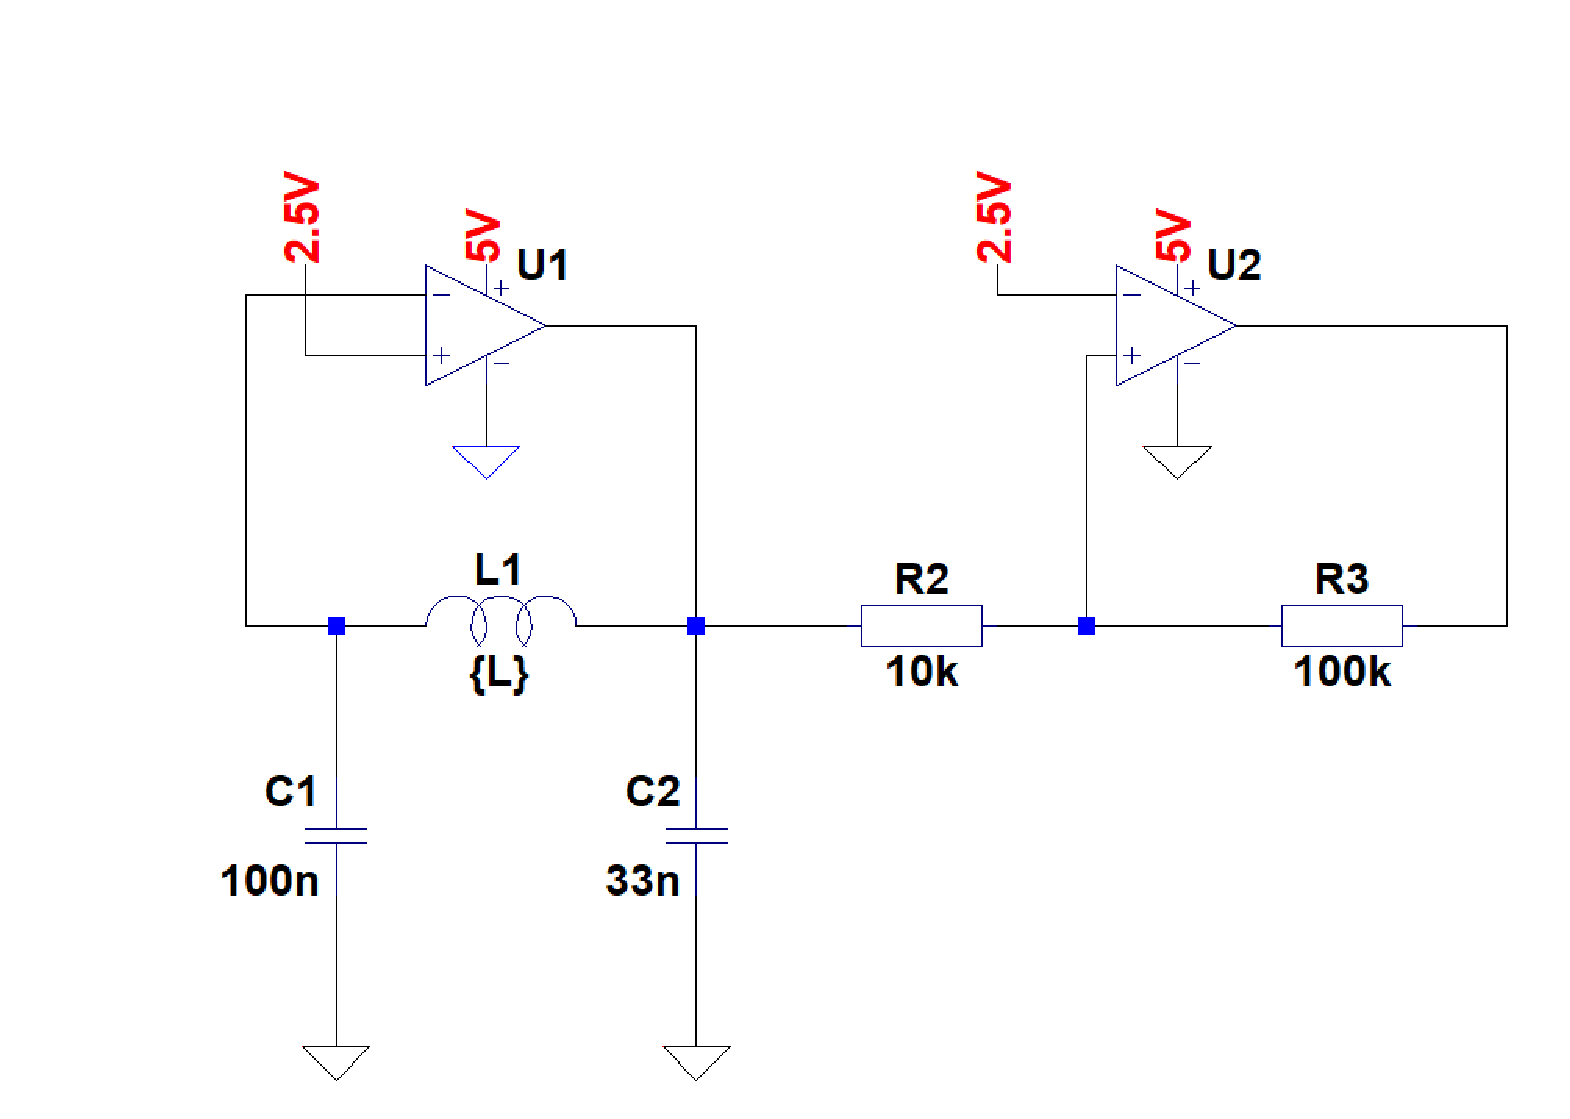
\includegraphics[width=1\linewidth]{fahrzeugerkennung/Colpitts_schmitt.pdf}
    \caption{Colpitts Oszillator mit Schmitttrigger}
\end{figure}

Als Komparator haben wir den LM393D IC ausgewählt, da er sehr günstig ist und weil er in SMD Form zwei Komparatoren in einem Package hat. Er ist jedoch ein sogenannter Open-Collector IC. Das heißt er kann seinen Ausgang nur auf Masse schalten und er braucht daher 
einen Pullup-Widerstand auf eine positive Spannung um das gewünschte Rechtecksignal zu erzeugen. Diese Widerstände sind in der folgenden Abbildung mit $RCP1$ und $RCP2$ gekennzeichnet

\begin{figure}[H]
    \centering
    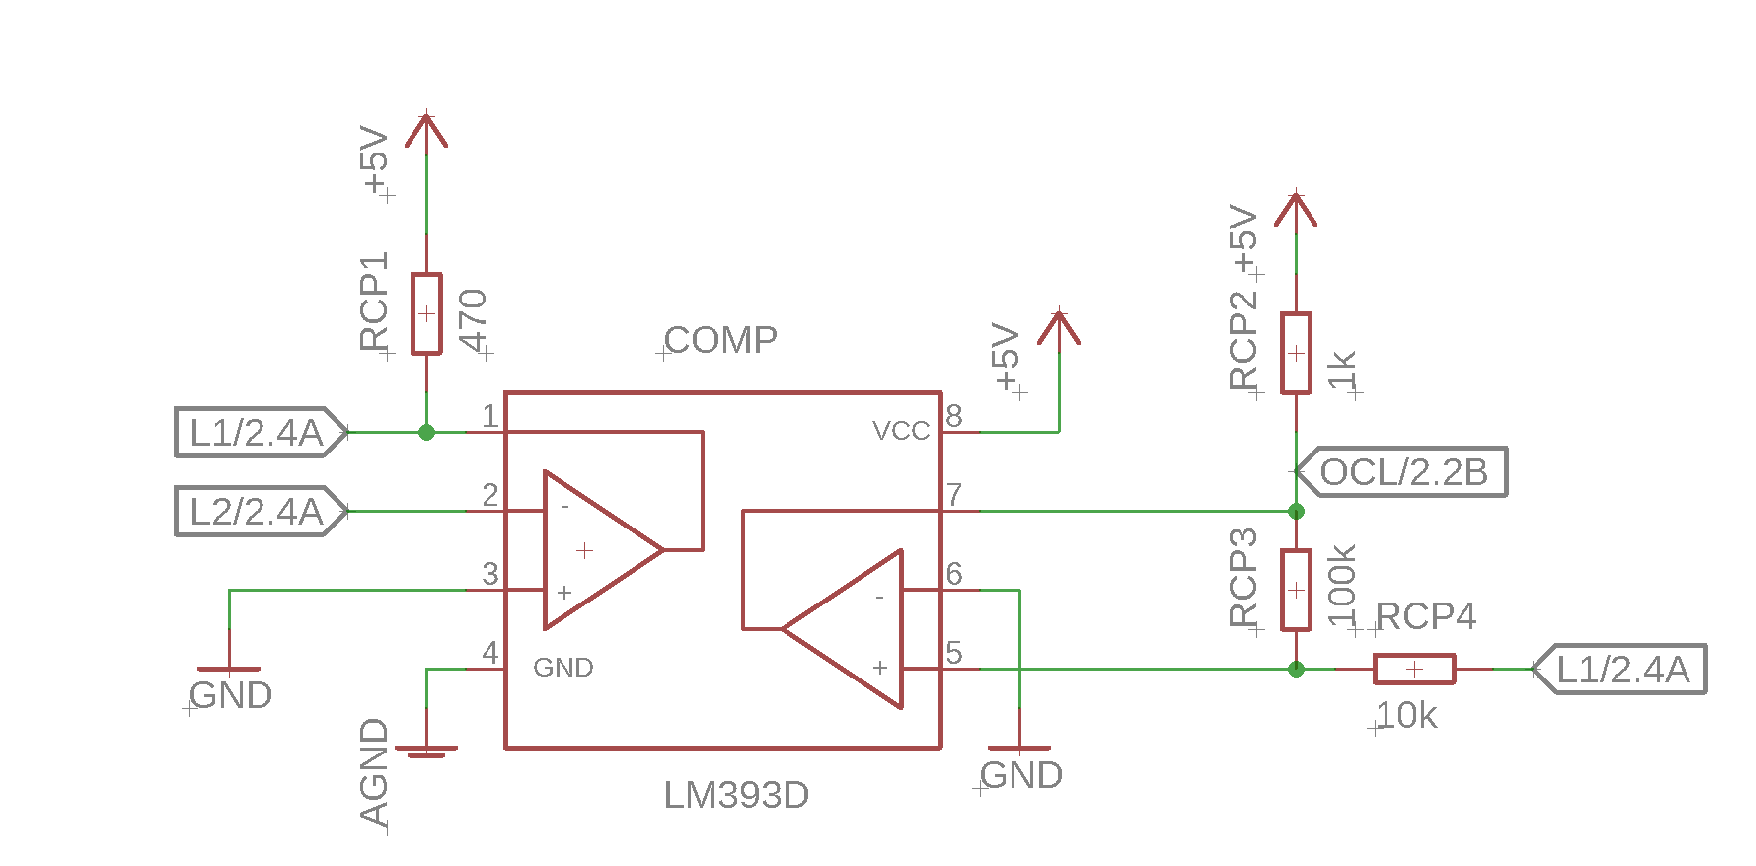
\includegraphics[width=0.8\linewidth]{fahrzeugerkennung/LM393D_eagle.pdf}
    \caption{LM393D im Slave Schaltplan}
\end{figure}

Als Kondensatoren des Colpitts-Oszillator wurden die Werte $\SI{100}{\nano\farad}$ und $\SI{33}{\nano\farad}$ verwendet. Dies ist wichtig um die Resonanzfrequenz des Oszillators zu bestimmen.
Für eine Spule mit einer Induktivität von $\SI{50}{\micro\henry}$ würde sich eine Frequenz nach der Gleichung \ref{eq:colpitts} von $\SI{148,165}{\kilo\hertz}$ ergeben. 

\begin{figure}[H]
    \centering
    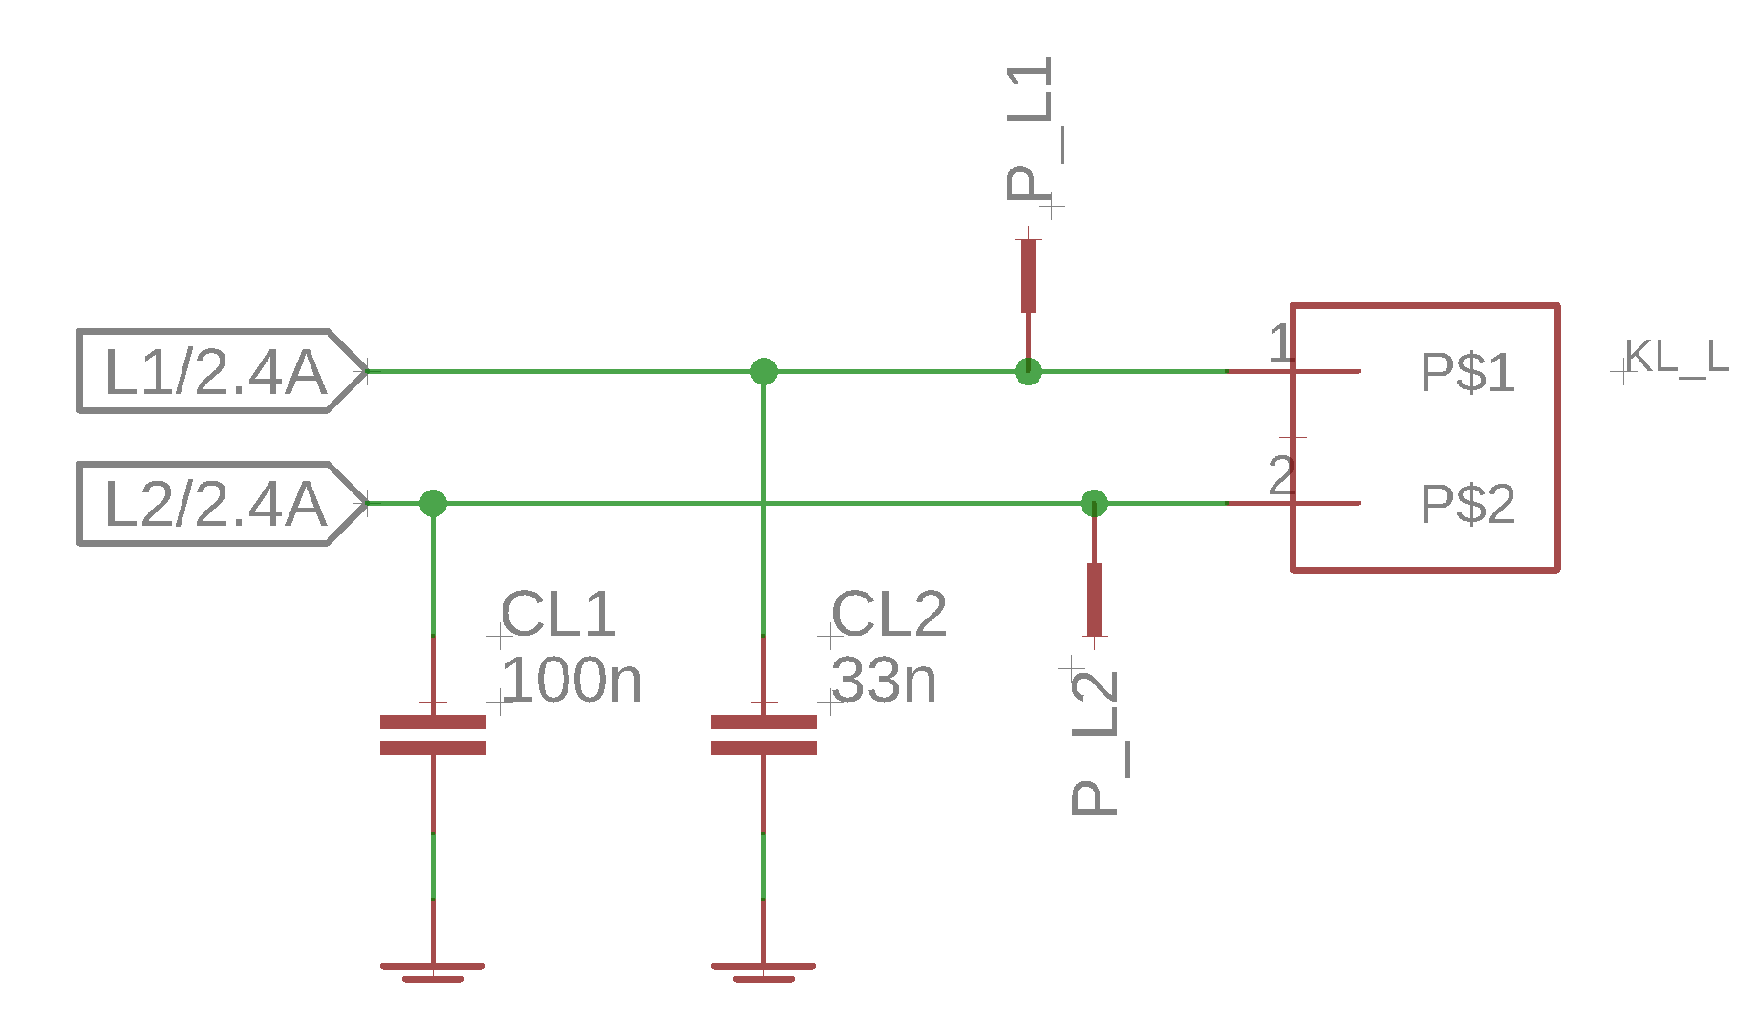
\includegraphics[width=0.6\linewidth]{fahrzeugerkennung/colpitts_capacitors_eagle.pdf}
    \caption{Colpitts Kondensatoren im Slave Schaltplan}
\end{figure}

Die Spule wird an den mit 'L' beschrifteten Anschlussist angeschlossen (Siehe Abbildung \ref{fig:slave_front})

\subsubsection{Digitale Ein- und Ausgänge IO0 /IO1}

Sie haben generell verschiedene Anwendungsmöglichkeiten und sind daher je nach Kundenwunsch anpassbar. Derzeit werden sie als visuelle Indikatoren verwendet um direkt am Parkplatz anzuzeigen, ob er besetzt ist. 
Auf der Platine sind zwei LEDs verbaut, die immer den Zustand der IO-Pins anzeigen. Für den Parkplatz ist jedoch nötig die LEDs nach außen zu leiten. Dafür gibt es die Anschlüsse '0' und '1' die für IO0 und IO1 stehen, sowie die Anschlüsse
'+' und '-' die für $\SI{5}{\volt}$ und Masse stehen (Siehe Abbildung \ref{fig:slave_front}). Die Spannungsausgänge sind auch nützlich für externe Sensoren und Aktoren die nicht mehr wie $\SI{100}{\milli\ampere}$ brauchen.

\subsubsection{Weitere Anschlüsse}
\paragraph{Separater VCC Eingang}\mbox{} 

In der Entwicklungsphase hat es sich praktisch erwiesen einen eigenen Spannungsanschluss am Gerät anzubringen. Dieser ist an den Spannungsregler angeschlossen und muss mit $\SI{9}{\volt}$ bis $\SI{30}{\volt}$ vorsorgt werden.
Für den normalen Betrieb ist jedoch keine direkte Versorgung des Slaves mit Spannung nötig, da er seine Spannung über den RJ45 Stecker bezieht.

\begin{figure}[H]
    \centering
    \includegraphics[width=0.6\linewidth]{fahrzeugerkennung/uC_slave_left.pdf}
    \caption{Slave-Gerät mit Gehäuse von links}
    \label{fig:slave_left}
\end{figure}

\paragraph{RJ45 Anschlüsse}\mbox{} 

Wie im Absatz \ref{sec:func_adress_wire} erklärt müssen die Slaves in einer Kette verbunden werden um sie eindeutig zu identifizieren. Aus diesem Grund gibt es zwei RJ45-Stecker die die Slaves miteinander verbinden (Siehe Abbildung \ref{fig:bus_physical_overview}).

\paragraph{SPI Programmieranschluss}\mbox{} 

Um den Mikrocontroller zu programmieren braucht es einen Anschluss für einen externen Programmer, der den Maschinencode auf den hochlädt. Der Atmega328PB lässt eben über seine SPI Anschlüsse programmieren welche im folgenden Bild
an den in rot gekennzeichneten Stecker geführt werden. 

\begin{figure}[H]
    \centering
    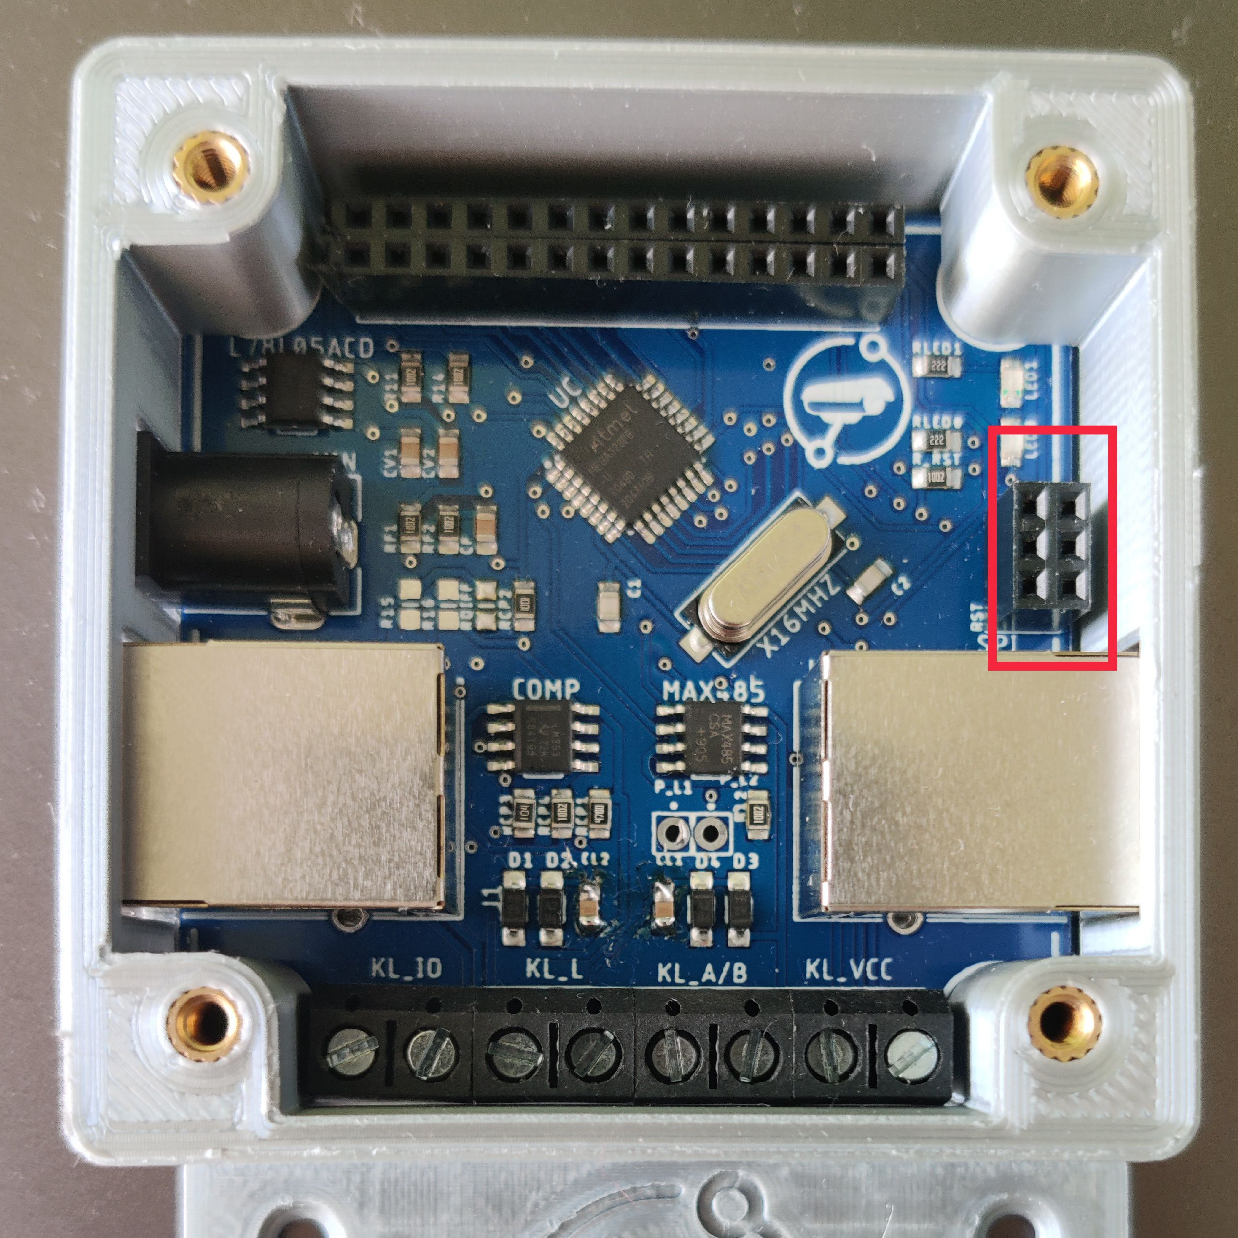
\includegraphics[width=0.6\linewidth]{fahrzeugerkennung/spi_marked.pdf}
    \caption{SPI Anschluss}
    \label{fig:slave_left}
\end{figure}

In gleicher Orientation wie in Abbildung \ref{fig:slave_left} gilt die folgende Netzbeschriftung.

\begin{table}[H]
    \centering
    \begin{tabular}{|c|c|}
        \hline
        MISO & +5V  \\ \hline
        SCK  & MOSI \\ \hline
        RST  & GND  \\ \hline
    \end{tabular}
    \caption{Netzbelegung des SPI Anschluss}
\end{table}

\subsubsection{Atmega328PB}
\paragraph{Zuweisung der Pins}\mbox{} 

\begin{figure}[H]
    \centering
    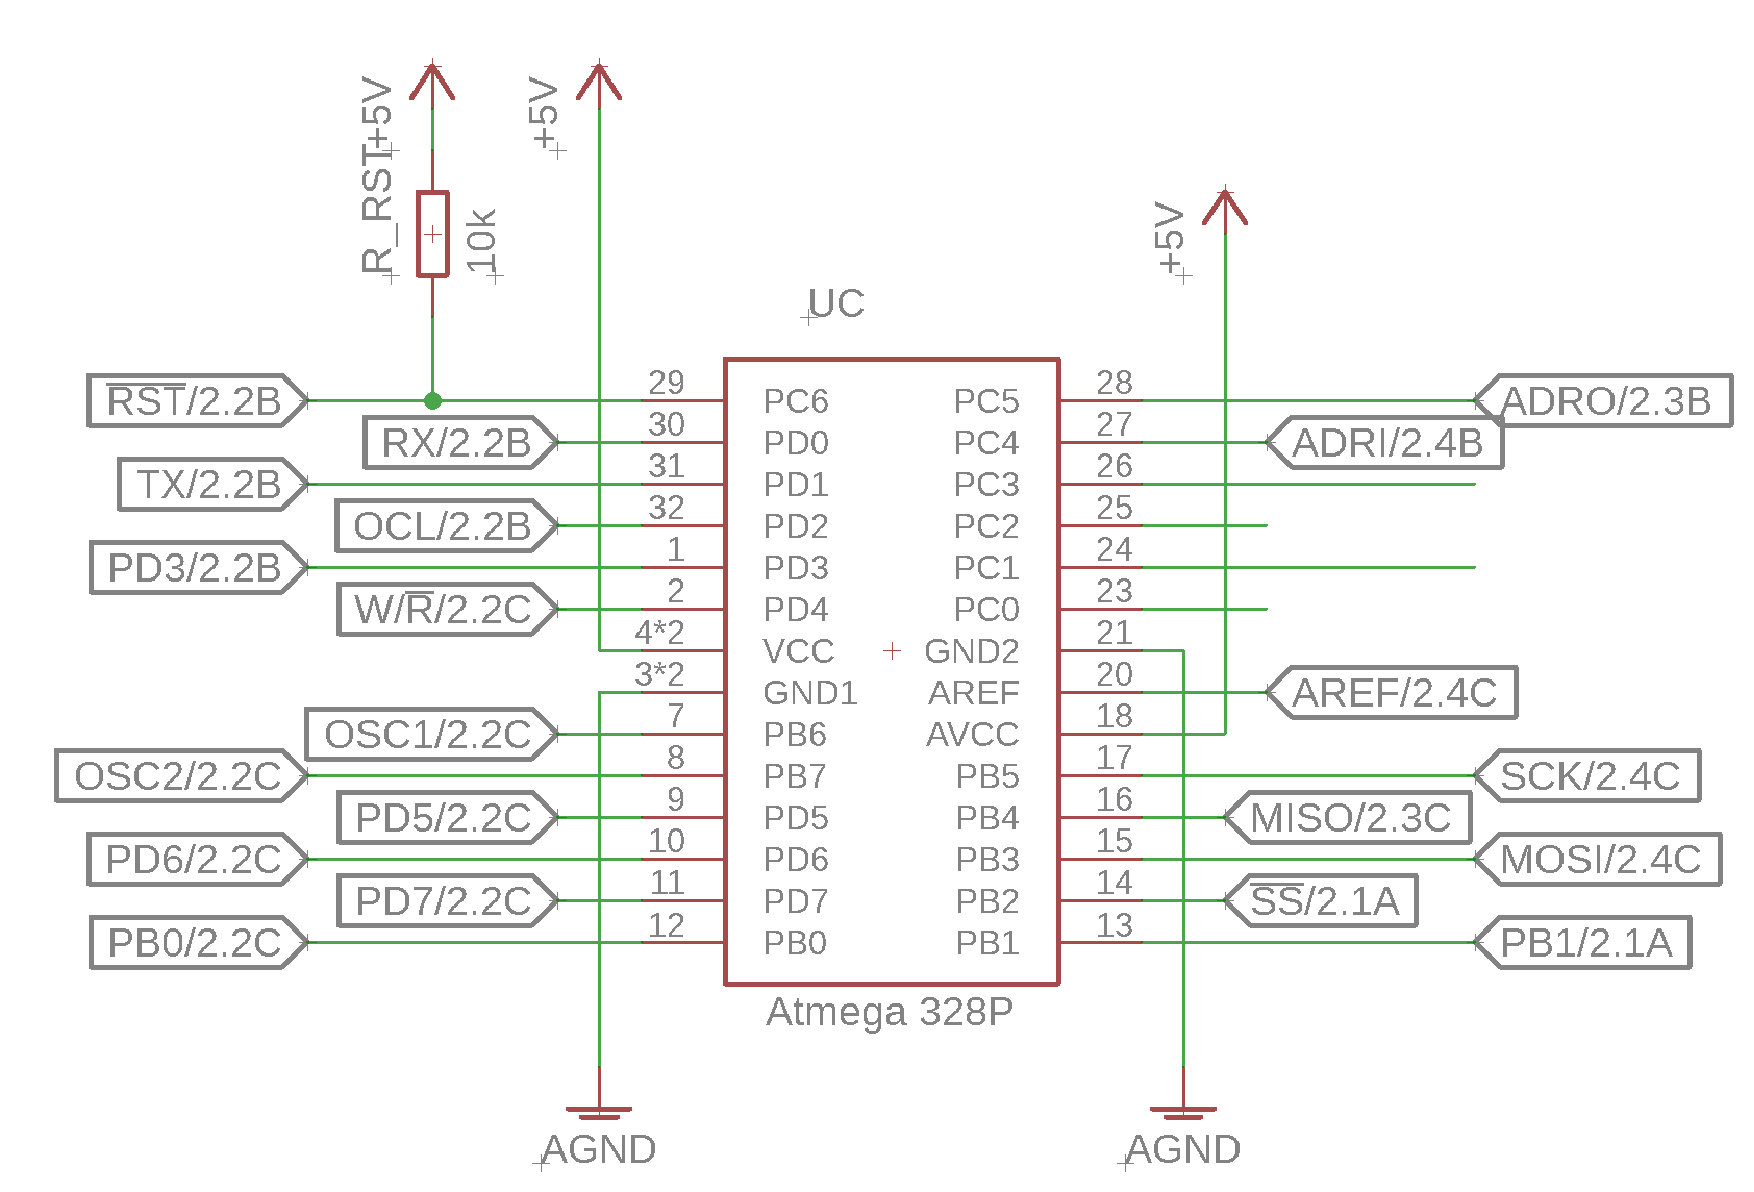
\includegraphics[width=0.6\linewidth]{fahrzeugerkennung/Atmega328PB_pinout.pdf}
    \caption{Pin-Netz Zuordnung des Atmega328PB im Slave Schaltplan}
\end{figure}

\paragraph{Fuse-Bits und Quartz}\mbox{} 

Unter Fuse-Bits versteht man Bits die nicht durch die Software des Mikrocontroller verändert werden können und zur Konfiguration des Mikrocontrollers dienen. Sie können nur durch einen externen Programmer verändert werden, 
wenn sie nicht schon vom Hersteller gesperrt worden sind. Es gibt insgesamt drei Fuse-Bytes, die für die Einstellungen des Atmega328PB zuständig sind. Sie regeln den internen Taktvorteiler, geben die Größe des Bootsektors an und
regeln neben anderen Sachen die Programmierung über SPI.

\begin{table}[H]
    \centering
    \begin{tabular}{|c|c|c|c|}
        \hline
        Fuse-Byte & \textbf{Low Fuse} & \textbf{Extended Fuse} & \textbf{High Fuse} \\ \hline
        Hex       & 0xFF              & 0xFD                   & 0xDA               \\ \hline
        Bin       & 1111 1111         & 1111 1101              & 1101 1010          \\ \hline
    \end{tabular}
    \caption{Konfiguration der Fuse Bits}
\end{table}


\begin{figure}[H]
    \centering
    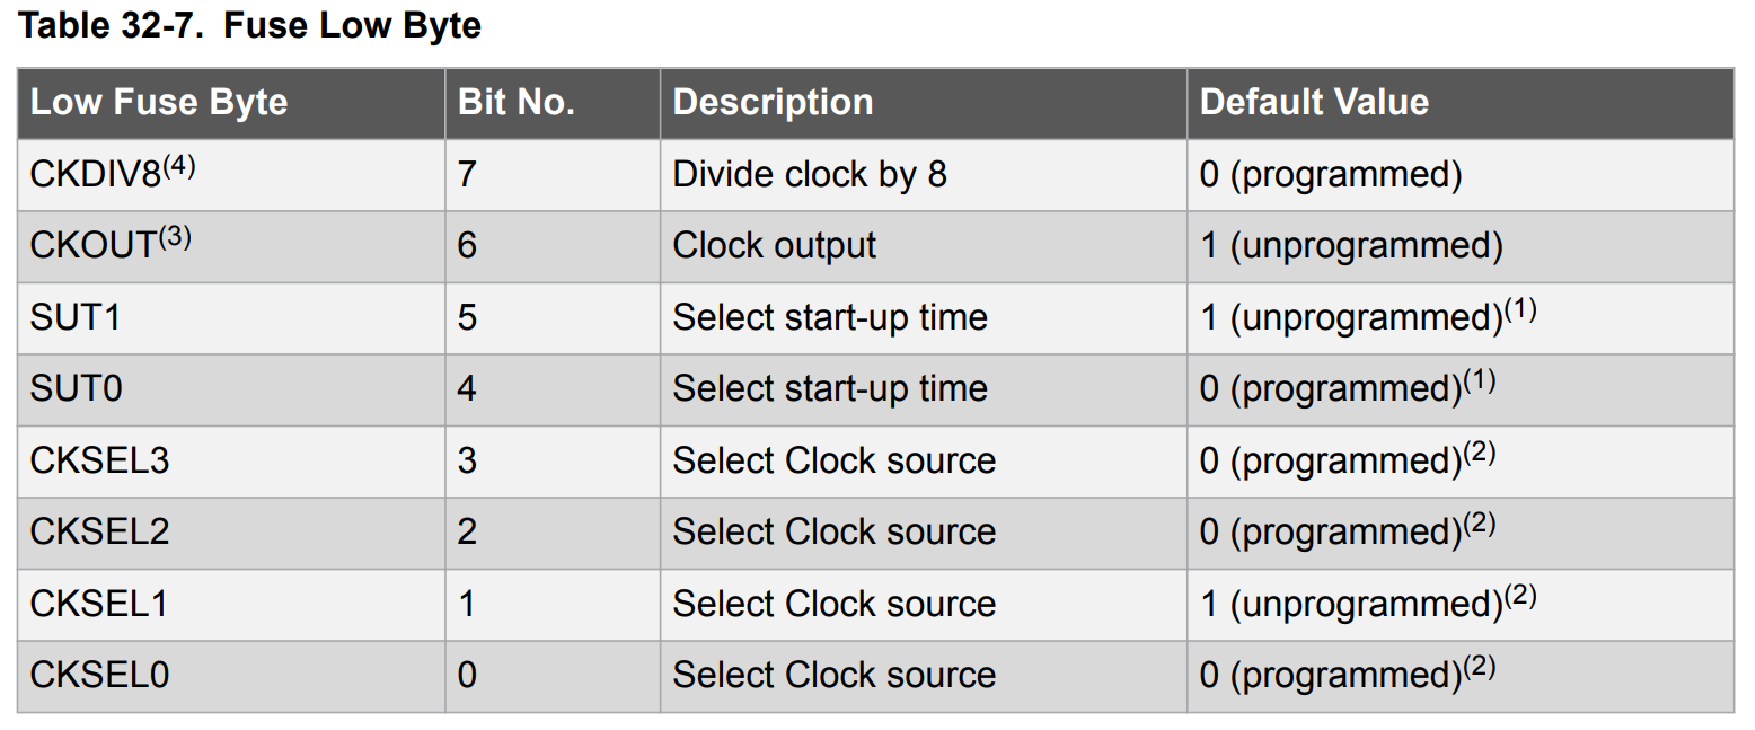
\includegraphics[width=1\linewidth]{fahrzeugerkennung/fuse_low_byte_datasheet.pdf}
    \caption{Low Fuse-Byte}
\end{figure}

Das Low-Byte gibt die Takteinstellungen vor. Der Slave ist auf einen externen $\SI{16}{\mega\hertz}$ Quartz angewiesen und er soll auch mit dieser Frequenz arbeiten. 
Der Taktteiler ist daher 1 welcher mit den Bit CKDIV = 1 eingestellt wurde. Die Taktquelle ist mit den Bits CKSEL0-3 auf einen externen Quartz umgestellt worden.

\begin{figure}[H]
    \centering
    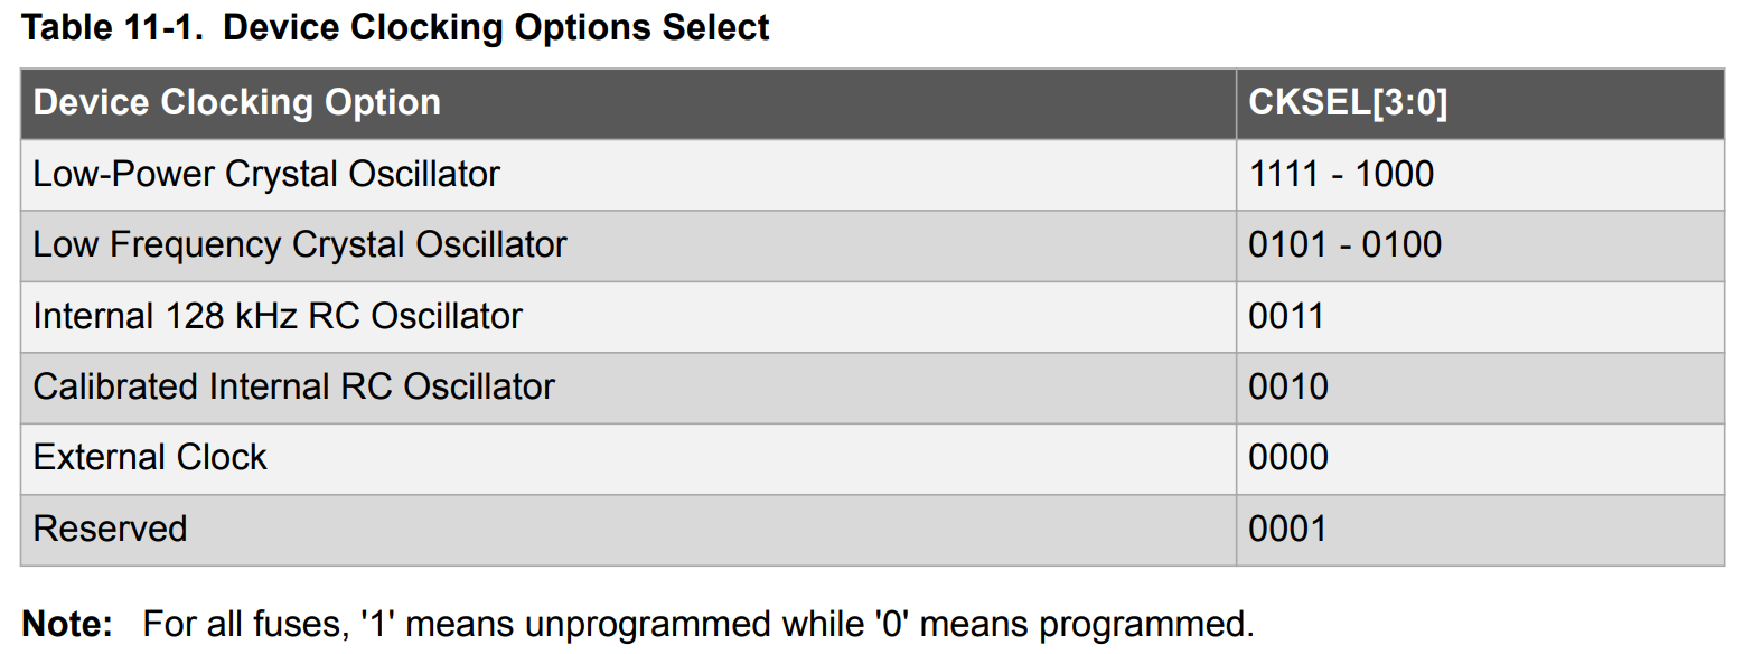
\includegraphics[width=1\linewidth]{fahrzeugerkennung/CKSEL_datasheet.pdf}
    \caption{Einstelleoptionen für den internen Takt des Atmega328PB}
\end{figure}

Wenn man weiter im Datenblatt liest erhält man die Werte für die Trimmkondensatoren, nämlich jeweils $\SI{22}{\nano\farad}$.

\begin{figure}[H]
    \centering
    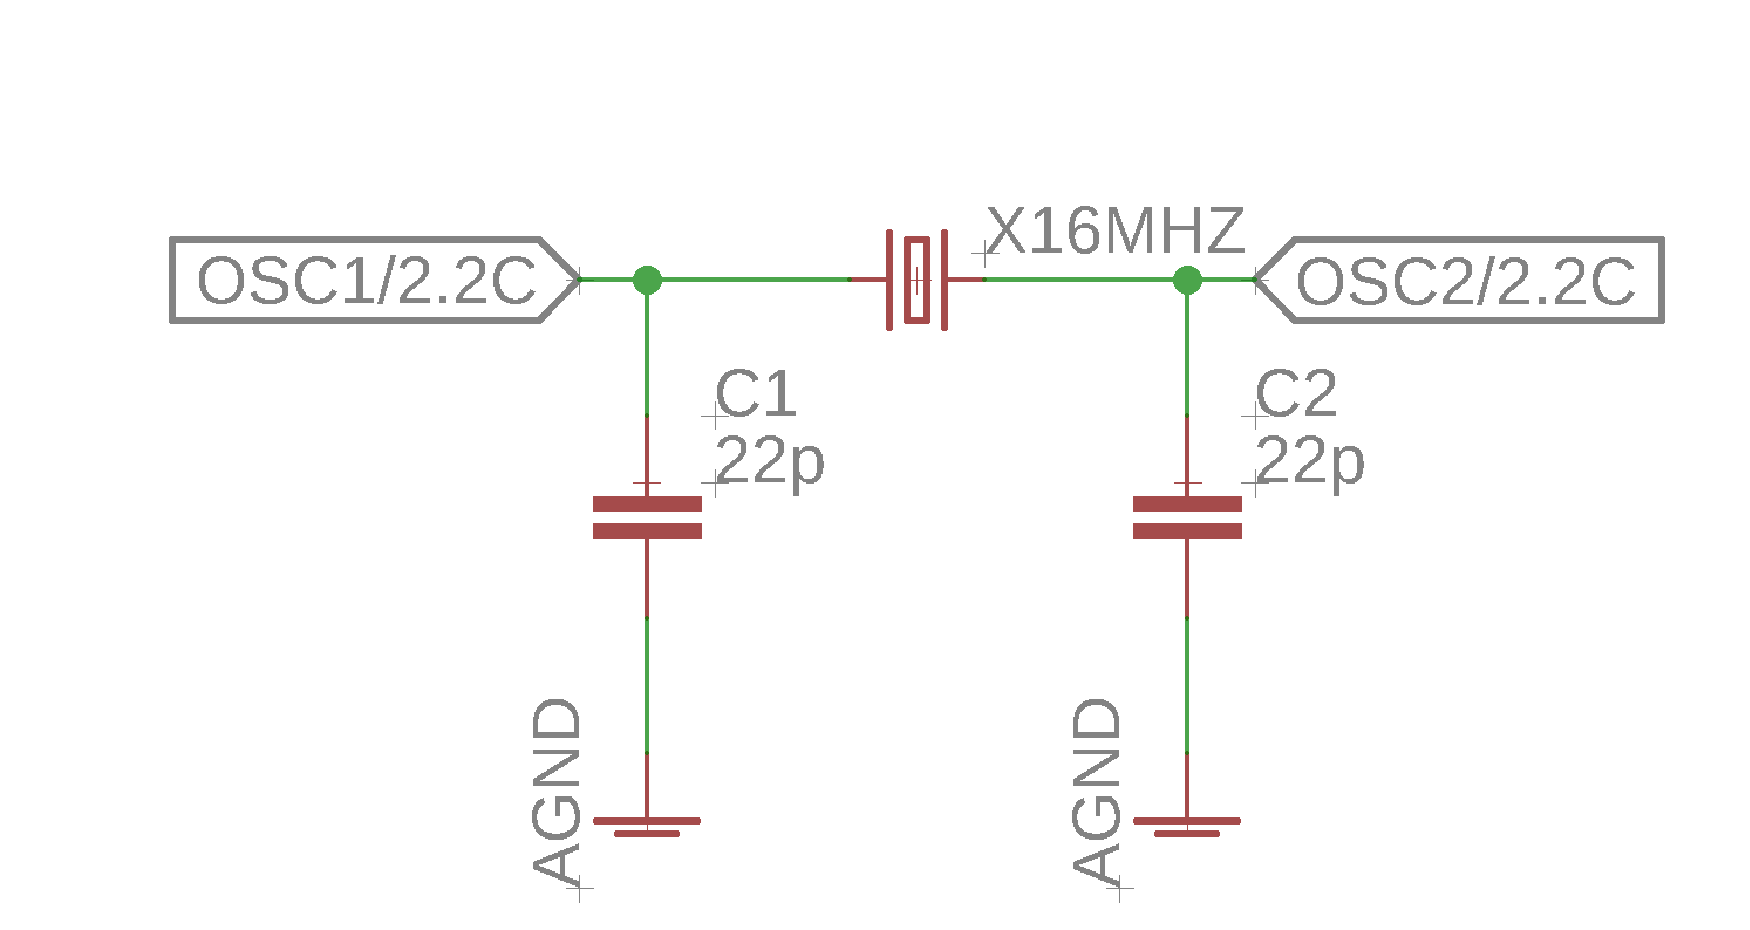
\includegraphics[width=0.6\linewidth]{fahrzeugerkennung/quartz_schaltplan.pdf}
    \caption{Quartz im Slave Schaltplan}
\end{figure}



\begin{figure}[H]
    \centering
    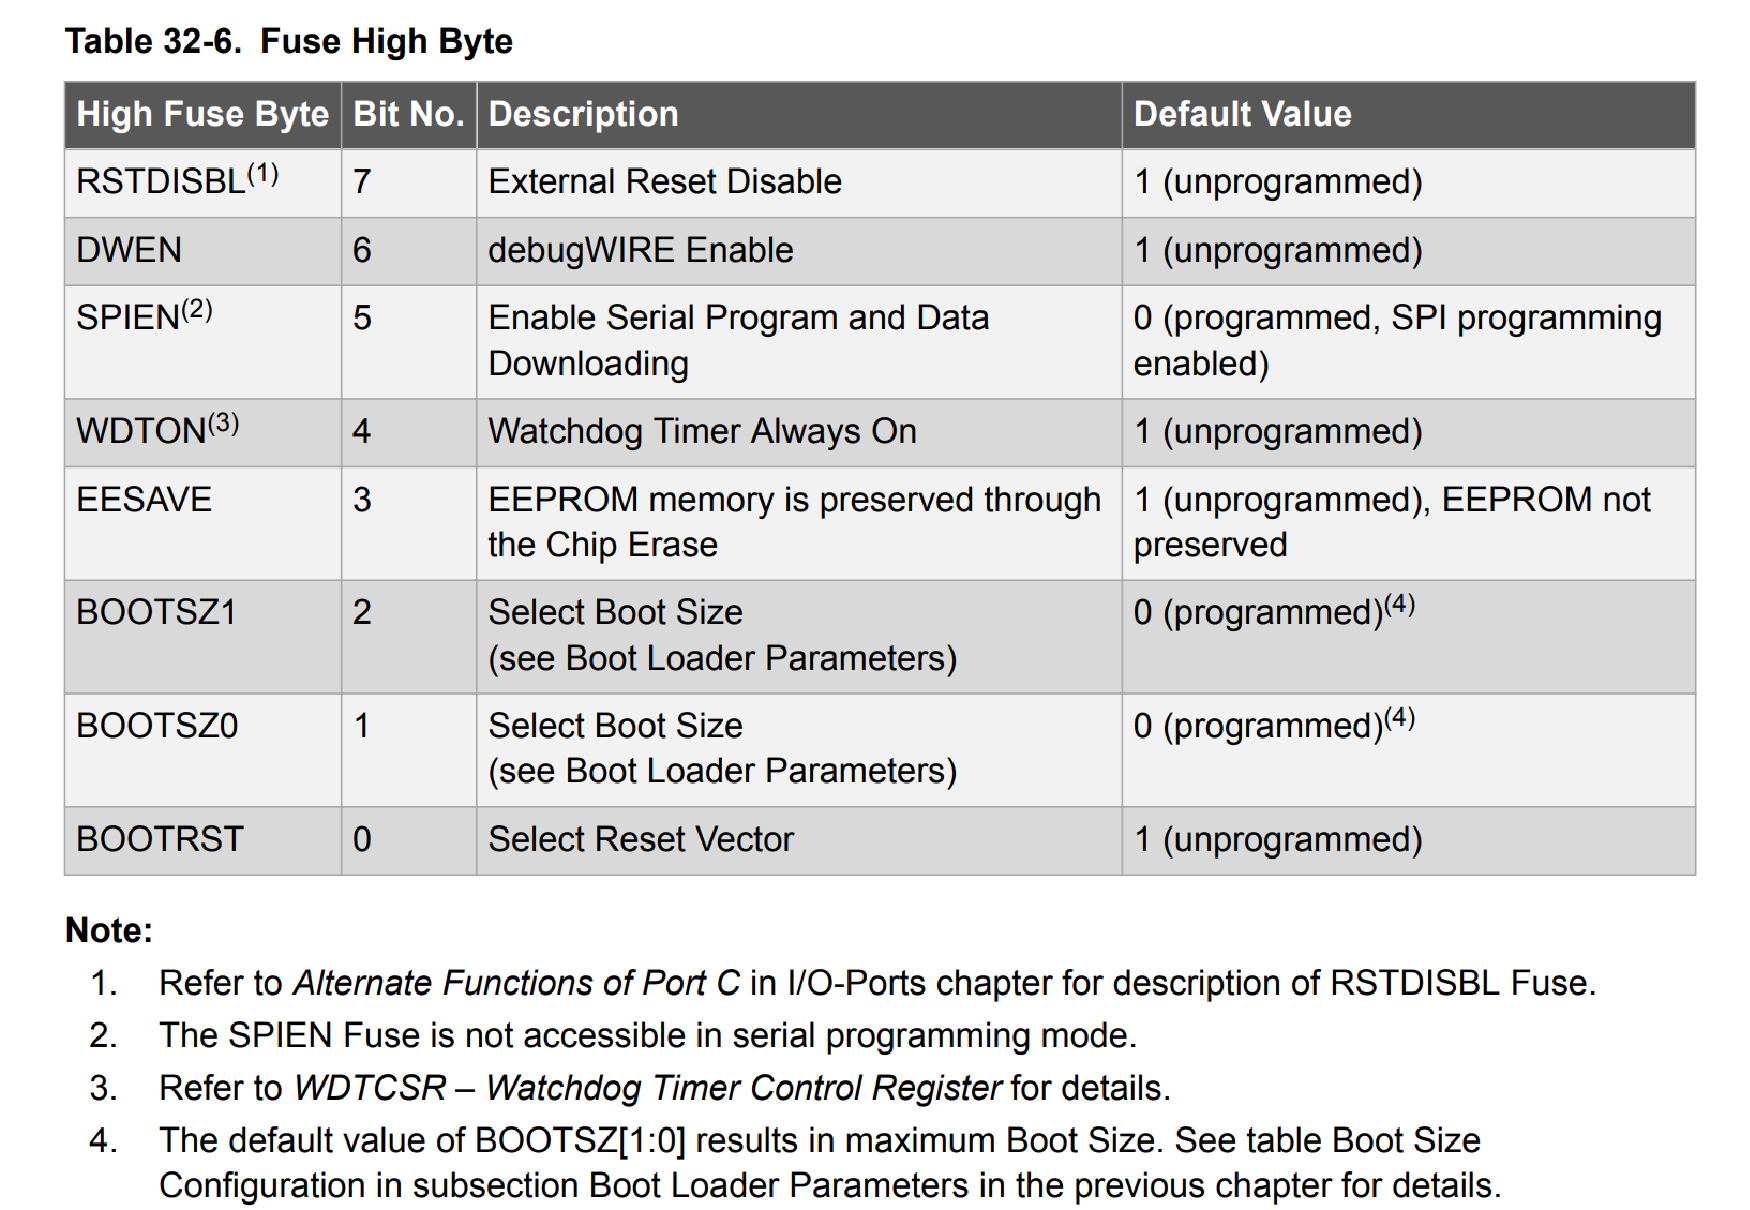
\includegraphics[width=1\linewidth]{fahrzeugerkennung/fuse_high_byte_datasheet.pdf}
    \caption{High Fuse-Byte}
\end{figure}

Hier ist zu beachten, dass das Bit SPIEN auf 0 gesetzt sein muss, damit ein externer SPI-Programmer verwendet werden kann. Wird dieses Bit auf 1 gesetzt kann das nur schwer rückgängig gemacht werden.

\begin{figure}[H]
    \centering
    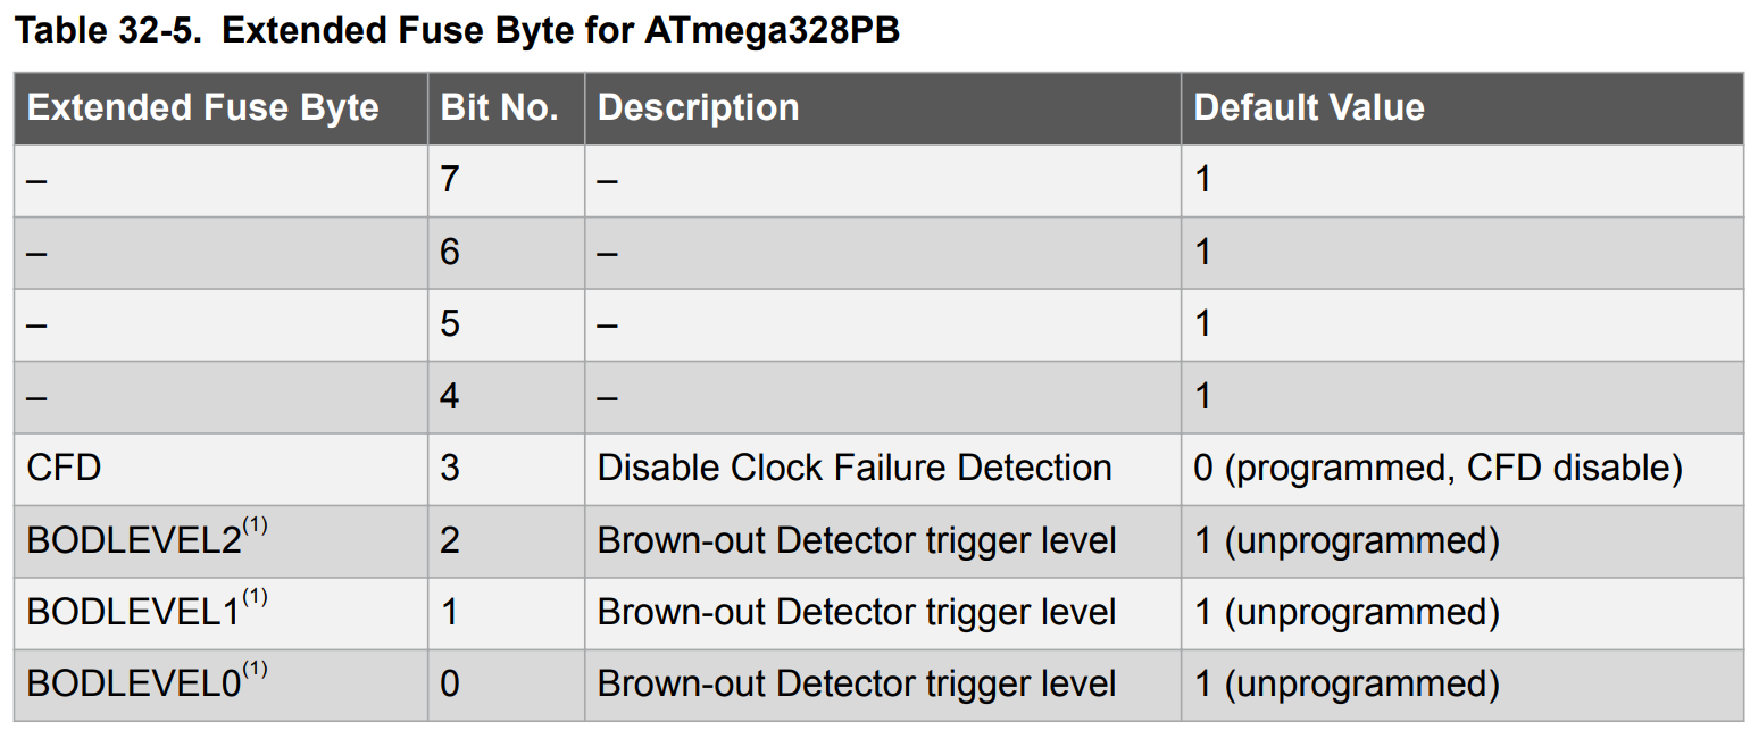
\includegraphics[width=1\linewidth]{fahrzeugerkennung/fuse_extended_byte_datasheet.pdf}
    \caption{Extended Fuse-Byte}
\end{figure}

Mit diesem Byte wird der Brownout Reset Spannungspegel festgelegt. Wenn die Versorgungsspannung des Atmega328PB unter diesen Wert fällt bricht der Mikrocontroller seine Operation ab und setzt sich zurück.


\paragraph{SPI-Programmierung}\mbox{} 

Es gibt viele Möglichkeiten einen Mikrocontroller mit unterschiedlichen Werkzeugen zu programmieren. Eine Variante ist die mit den unten verwendeten Werkzeugen.

\begin{itemize}
    \item \textbf{AVRDUDE} \\
    AVRDUDE\footnote{\url{https://www.mikrocontroller.net/articles/AVRDUDE}} ist eine Programmiersoftware für Mikrocontroller aus der Microchip-AVR Familie. Sie hat keine Benutzeroberfläche, sondern nur eine Terminalausgabe.
    \item \textbf{PlatformIO} \\
    PlatformIO ist Erweiterung für Visual Studio Code, die es ermöglicht Mikrokontroller Projekte zu entwickeln. Sie bietet auch die Möglichkeit an, bereits existierende Compiler oder Programmiersoftware wie AVRDUDE zu verwenden.
    \item \textbf{Arduino UNO als Programmer} \\
    Der Arduino Uno ist ein Mikrocontroller basiertes Board, welches weit verbreitet ist und für das es große Softwareunterstützung gibt. Eine mögliche Anwendung dieses Boards ist die eines SPI-Programmer. 
    Dazu muss aber zuerst die richtige Software auf den Arduino hochgeladen werden. Dafür braucht man die zum Arduino zugehörige Arduino Entwicklungsumgebung.
    \begin{figure}[H]
        \centering
        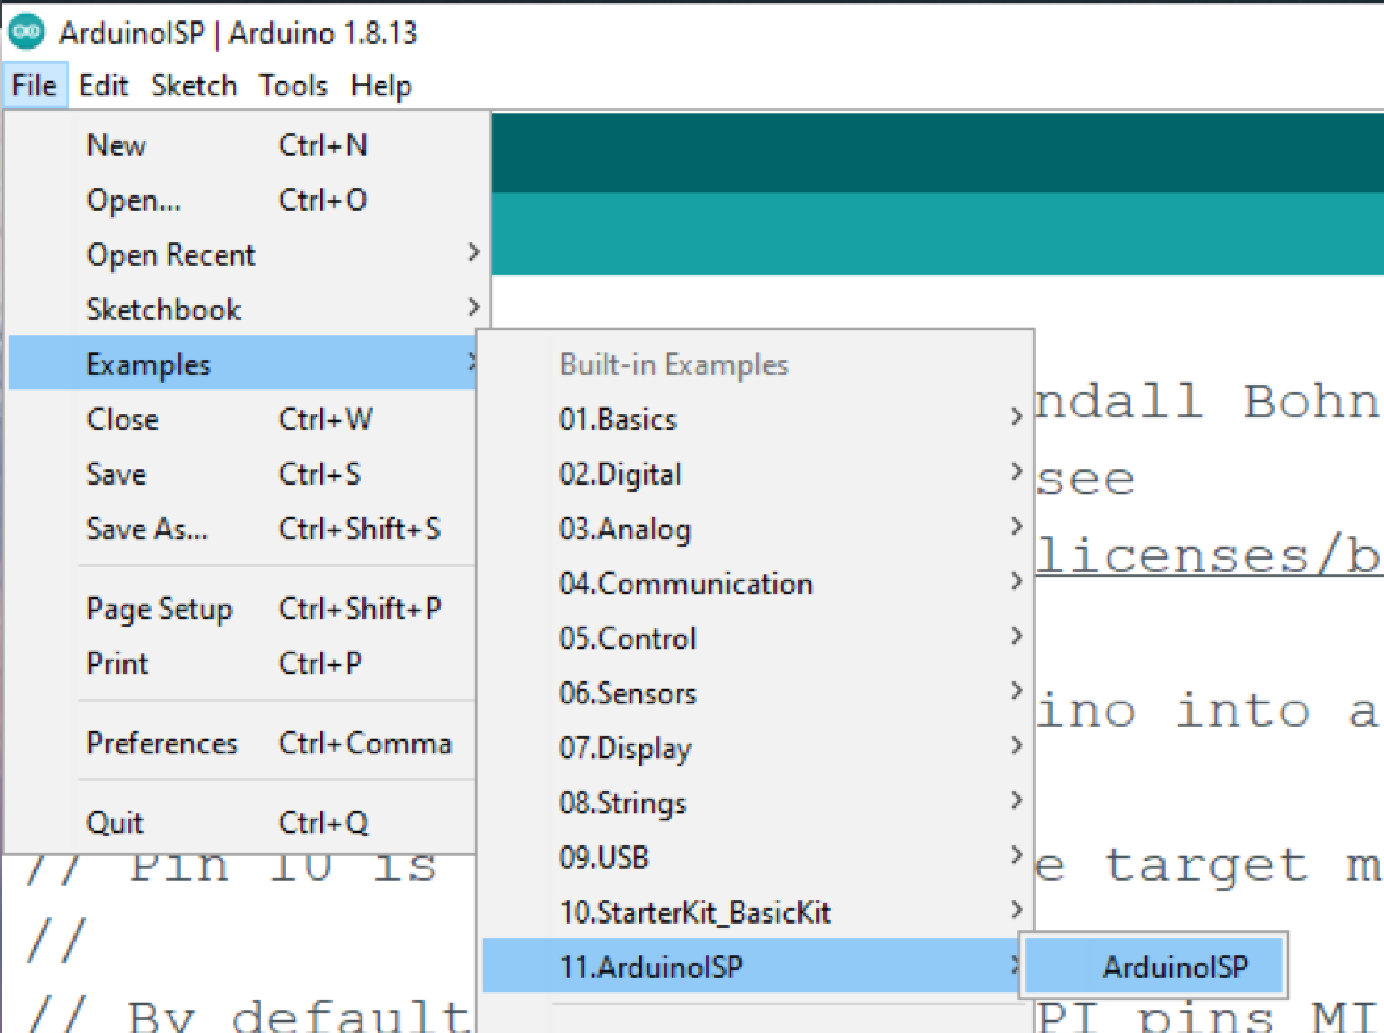
\includegraphics[width=0.4\linewidth]{fahrzeugerkennung/open_arduinoISP_sketch.pdf}
        \caption{ArduinoISP Sketch auswählen}
    \end{figure}
    Der ArduinoISP Sketch macht den Arduino UNO zu einem AVR Programmer. Dieser Sketch muss dann kompiliert und hochgeladen werden. Dafür sind die in der folgenden Abbildung Einstellungen zu beachten. Der COM-Anschluss kann
    bei anderen Computern anders sein und sollte immer selbst bestimmt werden. 
    \begin{figure}[H]
        \centering
        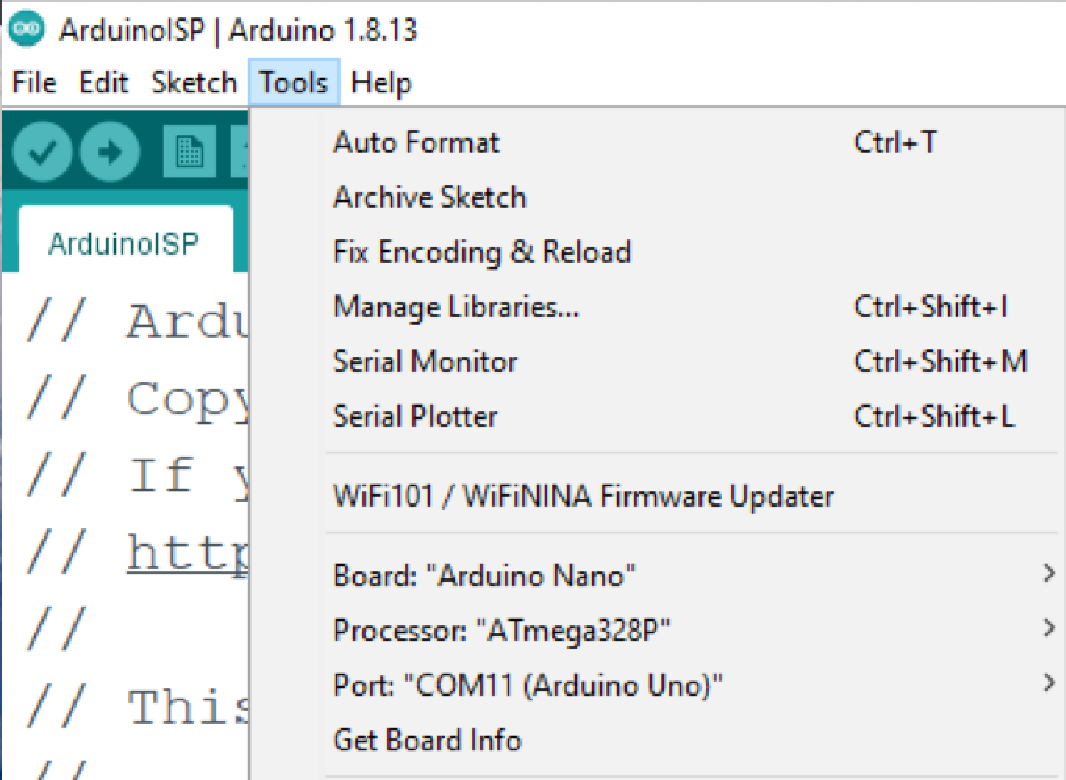
\includegraphics[width=0.4\linewidth]{fahrzeugerkennung/arduino_upload_Settings.pdf}
        \caption{Arduino Upload Einstellungen für ArduinoISP Sketch}
    \end{figure}
\end{itemize}

Wenn der Arduino als SPI-Programmer kann er wir im unteren Bild an den Slave angeschlossen werden.

\begin{figure}[H]
    \centering
    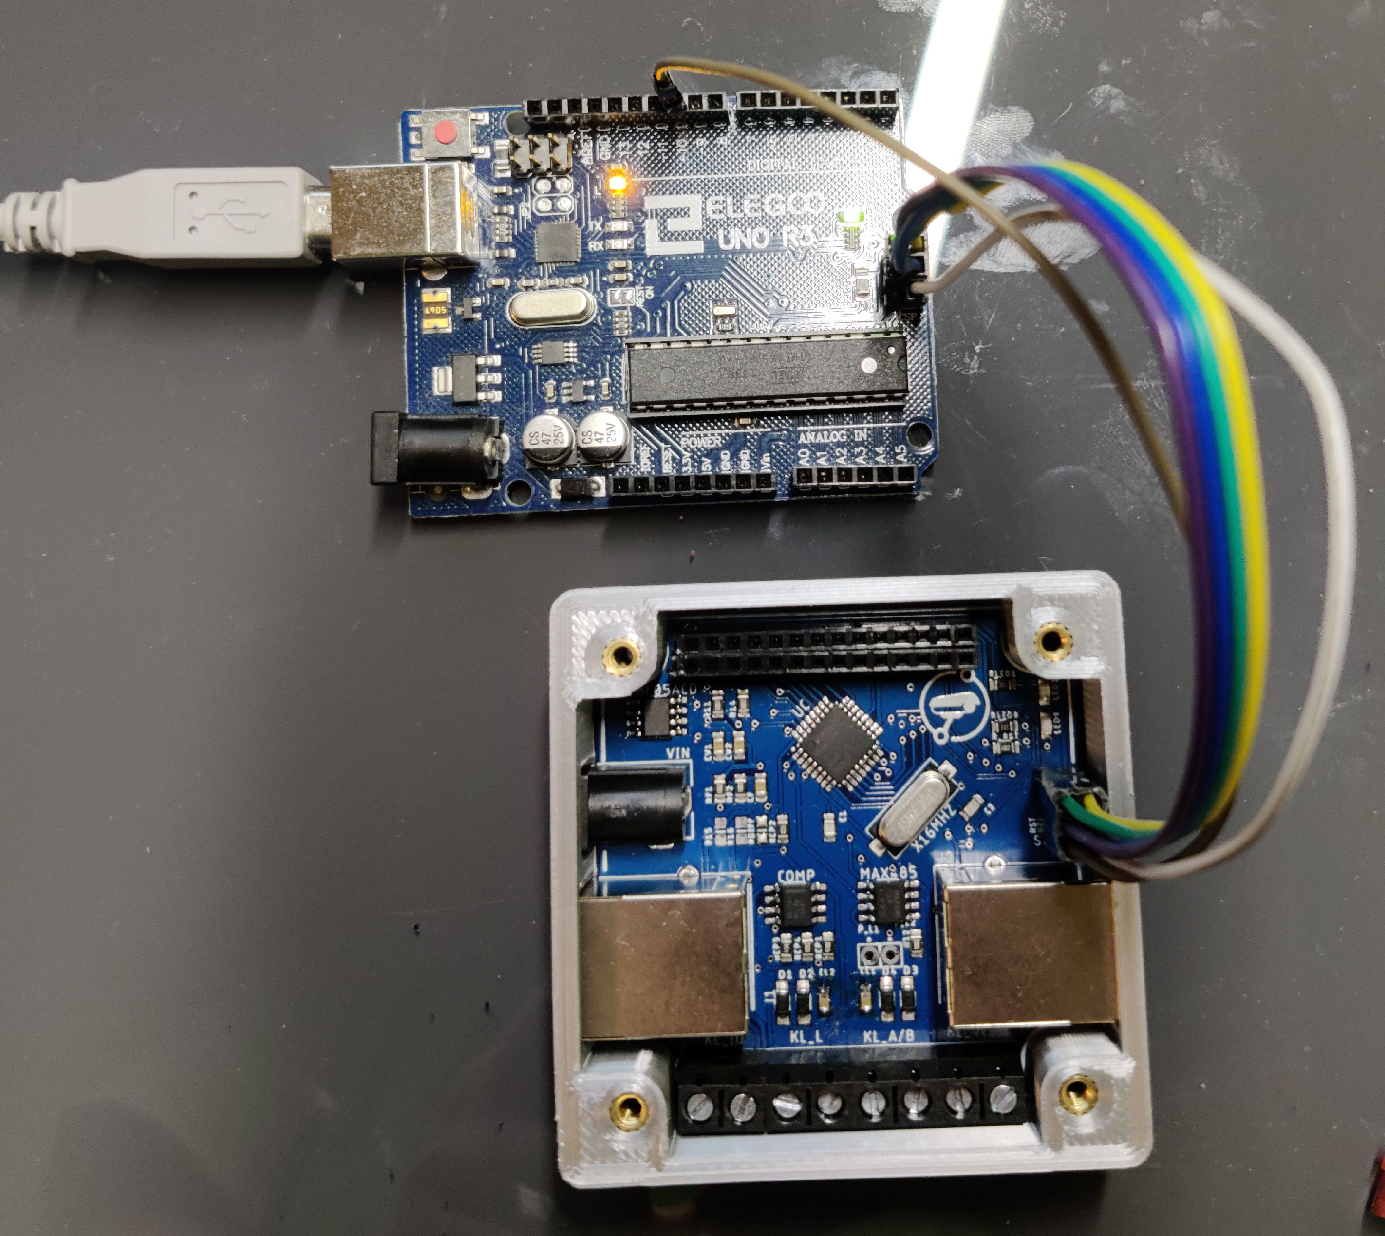
\includegraphics[width=0.6\linewidth]{fahrzeugerkennung/spi_prgramming.pdf}
    \caption{Anschluss eines externen SPI Programmer}
\end{figure}

Um die Fuse-Bits zu setzen ist es nötig AVRDUDE einmal mit den folgenden Parametern zu starten. Es muss zuerst wieder der COM-Anschluss des Arduino am Computer ermittelt werden.

\begin{listing}[H]
    \begin{minted}{shell}
    -U efuse:w:0xfd:m -U lfuse:w:0xff:m -U hfuse:w:0xda:m -e -v -p m328pb -c arduino -PCOM11 -b19200 -D -C"C:\Program Files (x86)\Arduino\hardware\tools\avr\etc\avrdude.conf"
    \end{minted}
    \caption{AVRDUDE Argumente für die Fuse-Bits}
\end{listing}

Damit man  in Visual Studio Code über PlatformIO kompilieren und hochladen kann sind die folgenden Einstellung in der platformio.ini Datei zu treffen.


\begin{listing}[H]
    \begin{minted}{Ini}
    [env:ATmega328PB]
    platform = atmelavr
    board = ATmega328PB
    framework = arduino
    upload_port = COM11
    upload_protocol = stk500v1
    upload_speed = 19200
    board_build.F_cpu = 16000000L
    board_fuses.lfuse = 0xFF
    board_fuses.hfuse = 0xDA
    board_fuses.efuse = 0xFD
    upload_flags = 
    -PCOM11
    -b$UPLOAD_SPEED
    -e
    \end{minted}
    \caption{PlatformIO Einstellungen}
\end{listing}
\subsubsection{Software des Slaves}
\paragraph{Konfiguration der Register}\mbox{} 

Die Funktionen der Registerwerte wurden in den Code-Komentaren hinterlegt.
\begin{listing}[H]
    \begin{minted}{C}
    void init()
    {
        DDRC &= ~(1 << DDC4) & ~(1 << DDC5);      //ADRO und ADRI als Eingang 
        DDRB |= (1 << PORTB1) | (1 << PORTB2);    //IO0 und IO1 als Ausgang
    
        PORTB &= ~(1<< PORTB2) & ~(1 << PORTB1);  //IO0 und IO1 auf logisch 0 legen.
        PORTC |= (1 << PORTC4) | (1 << PORTC5);   //Pullupwiderstände von ADRO und ADRI einschalten
        
        rs485_init(56700, P_NONE, S_1, F_CPU);
        reset();
    }
    \end{minted}
    \caption{allgemeine Registereinstellungen}
\end{listing}

\begin{listing}[H]
    \begin{minted}{C}
    TCCR1A = 0;                                             // OC1A Abschalten
    TCCR1B |= (1 << CS10) | (1 << CS11) | (1 << WGM12);     // f-count = 250kHz, CTC
    OCR1A = 25000;                                          // f-ISR = 10Hz
    TIMSK1 |= (1 << OCIE1A);                                // Compare A interrupt
    \end{minted}
    \caption{Timer Registereinstellungen}
\end{listing}


\begin{listing}[H]
    \begin{minted}{C}
    uint16_t ubrr = ((internal_clk/8UL/baudrate) - 1);                      //UBRRL berechnen
    parity = ((parity & 0x02) << UPM01) | ((parity & 0x01) << UPM00);       //Paritöt fü UCSR0C bertechnen
    stopbit = ((stopbit & 0x01) << USBS0);                                  //Stopbit fü UCSR0C bertechnen
    UBRR0L = (char)ubrr;
    UBRR0H = (ubrr >> 8) & 0xFF;
    UCSR0A |= (1 << U2X0);
    UCSR0C |=  (0 << UMSEL01) | (0 << UMSEL00) | parity | stopbit | (1 << UCSZ01) | (1 << UCSZ00);         //Asynchron, Parität, Stopbits, 8 Datenits
    UCSR0B |=  (1 << RXCIE0) | (1 << RXEN0) | (1 << TXEN0);                 //Empfangsinterrupt, Empfang und Übertragung einschalten.      
    \end{minted}
    \caption{UART Registereinstellungen}
\end{listing}



\paragraph{UART Betrieb}\mbox{} 

Der Atmega328PB besitzt nur ein UART-Buffer mit einer Größe von einem Byte. Muss
zusätzlich per Software ein Ringbuffer mit Lesepointer pr und einem Schreibpointer pw erstellt
werden. Die Struktur des Buffers sieht so wie folgend aus.

\begin{figure}[H]
    \centering
    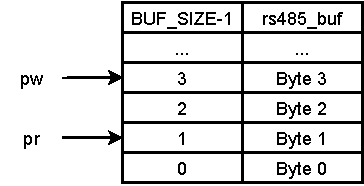
\includegraphics[width=0.6\linewidth]{fahrzeugerkennung/buffer.pdf}
    \caption{Slave UART-Buffer Struktur}
\end{figure}

Wenn ein neues Byte auf den Bus geschrieben wird lesen alle Slaves dieses Byte, mit dem UART-Empfangsinterrupt, in den Buffer an der Stelle des Schreibpointers. Dieser wird danach um eins
erhöht.


\begin{listing}[H]
    \begin{minted}{C}
    ISR(USART0_RX_vect)
    {
        rs485_buf[pw] = UDR0;
        pw = (pw + 1) % BUF_SIZE;
    }   
    \end{minted}
    \caption{Speichern eines Bytes auf den Buffer}
\end{listing}

\paragraph{Auswertung von Datenframes}\mbox{} 

Um die erhaltenen Datenframes überhaupt auslesen zu könen müssen sie erst im Buffer gefunden
werden. Die Bytes START, STOP und LF helfen dabei den Anfang und das Ende des Datenframes zu
finden. Zudem ist bekannt das ein Datenframe genau 16 Byte groß ist. Wenn der Lesepointer Schritt
für Schritt um 1 erhöht wird kann der Buffer solang durchgegangen werden bis ein Datenframe
gefunden wird. Diese Logik wird im folgenden Flussdiagramm verdeutlicht.

\begin{figure}[H]
    \centering
    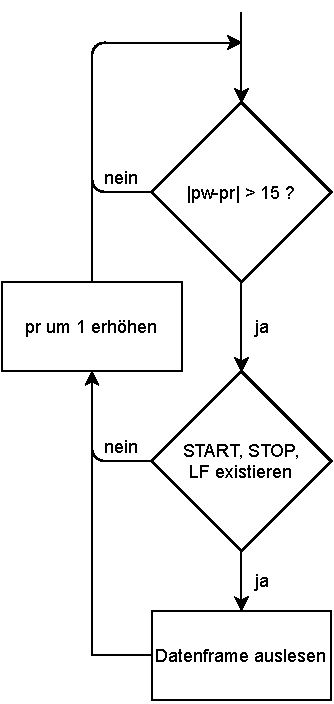
\includegraphics[width=0.4\linewidth]{fahrzeugerkennung/buffer_read_flochart.pdf}
    \caption{Flussdiagramm der Datenframeerkennung}
\end{figure}

Die ausgelesenen Daten werden in globale Variablen geschrieben, zusammen mit einem Flag
das bekannt gibt, dass ein neuer Dateframe angekommen ist. Infolge wird in der Hauptschleife
überprüft ob die Adresse mit der eigenen übereinstimmt. Wenn dies der Fall ist wird der Steuerbefehl
ausgeführt. Unten ist ein Beispielcode der bei der Änderung der eigenen Adresse ausgeführt wird.
\begin{listing}[H]
    \begin{minted}{C}
    else if(ADR_LSB == LOCAL_ADR_LSB && ADR_MSB == LOCAL_ADR_MSB)
    {
        if(controll_byte == ADR)
        {
        if(argument_1 == GIVE)
        {
            LOCAL_ADR_MSB = DATA[0];
            LOCAL_ADR_LSB = DATA[1];
            unsigned char response[8] = {LOCAL_ADR_MSB, LOCAL_ADR_LSB, 0, 0, 0, 0, 0, 0};
            rs485_write_frame(MASTER_MSB, MASTER_LSB, ADR, NONE, NONE,response);
        }
    }  
    \end{minted}
    \caption{ Auswertung der Daten eines Datenframes}
\end{listing}



\paragraph{Taktmessung}\mbox{} 

Der Master gibt bei der Taktmessung die Größe des Messzeitraumes in 10 \si{\milli\second} Auflösung an.
Die Aufgabe des Slaves ist es dann, über diesen Zeitraum die Takte des Rechtecksignals vom
Colpitts-Oszillator zu zählen. Dafür werden sowohl Timer als auch Eingangsflankeninterrupts
benötigt. Wenn der Slave die Anweisung zur Messung bekommt wird der folgenden Programmteil
aktiv.
\begin{listing}[H]
    \begin{minted}{C}
    else if(controll_byte == GET_FRQ)
    {
        measure_ms = argument_1;
        count_ticks = 0;
        count_ms_ticks = 0;
        MEASURE_ON;
        while(INT0_EN) {}
    
        unsigned char buf[] = "00000000";
        sprintf(buf, "%08lx", (unsigned long) count_ticks);
        rs485_write_frame(MASTER_MSB, MASTER_LSB, GET_FRQ, argument_1, NONE,buf);
    } 
    \end{minted}
    \caption{ Slave C-Code zur Taktmessung}
\end{listing}


Zuerst werden alle globalen Zählvariablen auf 0 zurückgesetzt und die Timer und Flankeninterrupts
eingeschalten. Das Programm wartet dann solange bis die Messung abgeschlossen ist und sendet
die Anzahl der Takte in ASCII kodiert an den Master zurück. 
\\ \\
\begin{listing}[H]
    \begin{minted}{C}
    else if(controll_byte == GET_FRQ)
    {
        measure_ms = argument_1;
        count_ticks = 0;
        count_ms_ticks = 0;
        MEASURE_ON;
        while(INT0_EN) {}
    
        unsigned char buf[] = "00000000";
        sprintf(buf, "%08lx", (unsigned long) count_ticks);
        rs485_write_frame(MASTER_MSB, MASTER_LSB, GET_FRQ, argument_1, NONE,buf);
    } 
    \end{minted}
    \caption{ Slave C-Code zur Taktmessung}
\end{listing}
Die Zählung der Takte funktioniert wie folgt.
\begin{listing}[H]
    \begin{minted}{C}
    ISR(INT0_vect)
    {
        count_ticks++;
    }
    \end{minted}
    \caption{ Slave C-Code zur Taktmessung}
\end{listing}


In der Flankeninterrupt Routine werden die Takte gezählt und in eine globale Variable geschrieben.
\begin{listing}[H]
    \begin{minted}{C}
    ISR(TIMER1_COMPA_vect)
    {
        count_ms_ticks++;
        if(count_ms_ticks >= measure_ms)
        {
            MEASURE_OFF;
            count_ms_ticks = 0;
        }
    }
    \end{minted}
    \caption{ Slave C-Code zur Taktmessung}
\end{listing}


In der Timerinterrupt Routine werden die Anzahl der Interrupts gezählt bis die gewünschte Messzeit
abgelaufen ist. Infolge werden die entsprechenden Interrupts wieder ausgeschalten.
\subsubsection{Layout des Slave-Gerätes}

Das Layout des Slaves wurde in Eagle\footnote{\url{https://www.autodesk.com/products/eagle/}} erstellt. Während der Entwicklungsphase gab es mehrere
Versionen des Slaves. In der ersten war das PCB nicht sehr platzeffizient und benutzte für den
Mikrocontroller keine SMD Variante. Unten ist ein Bild des ersten Prototyps mit bestückten Bauteilen
und Gehäuse.

\begin{figure}[H]
    \centering
    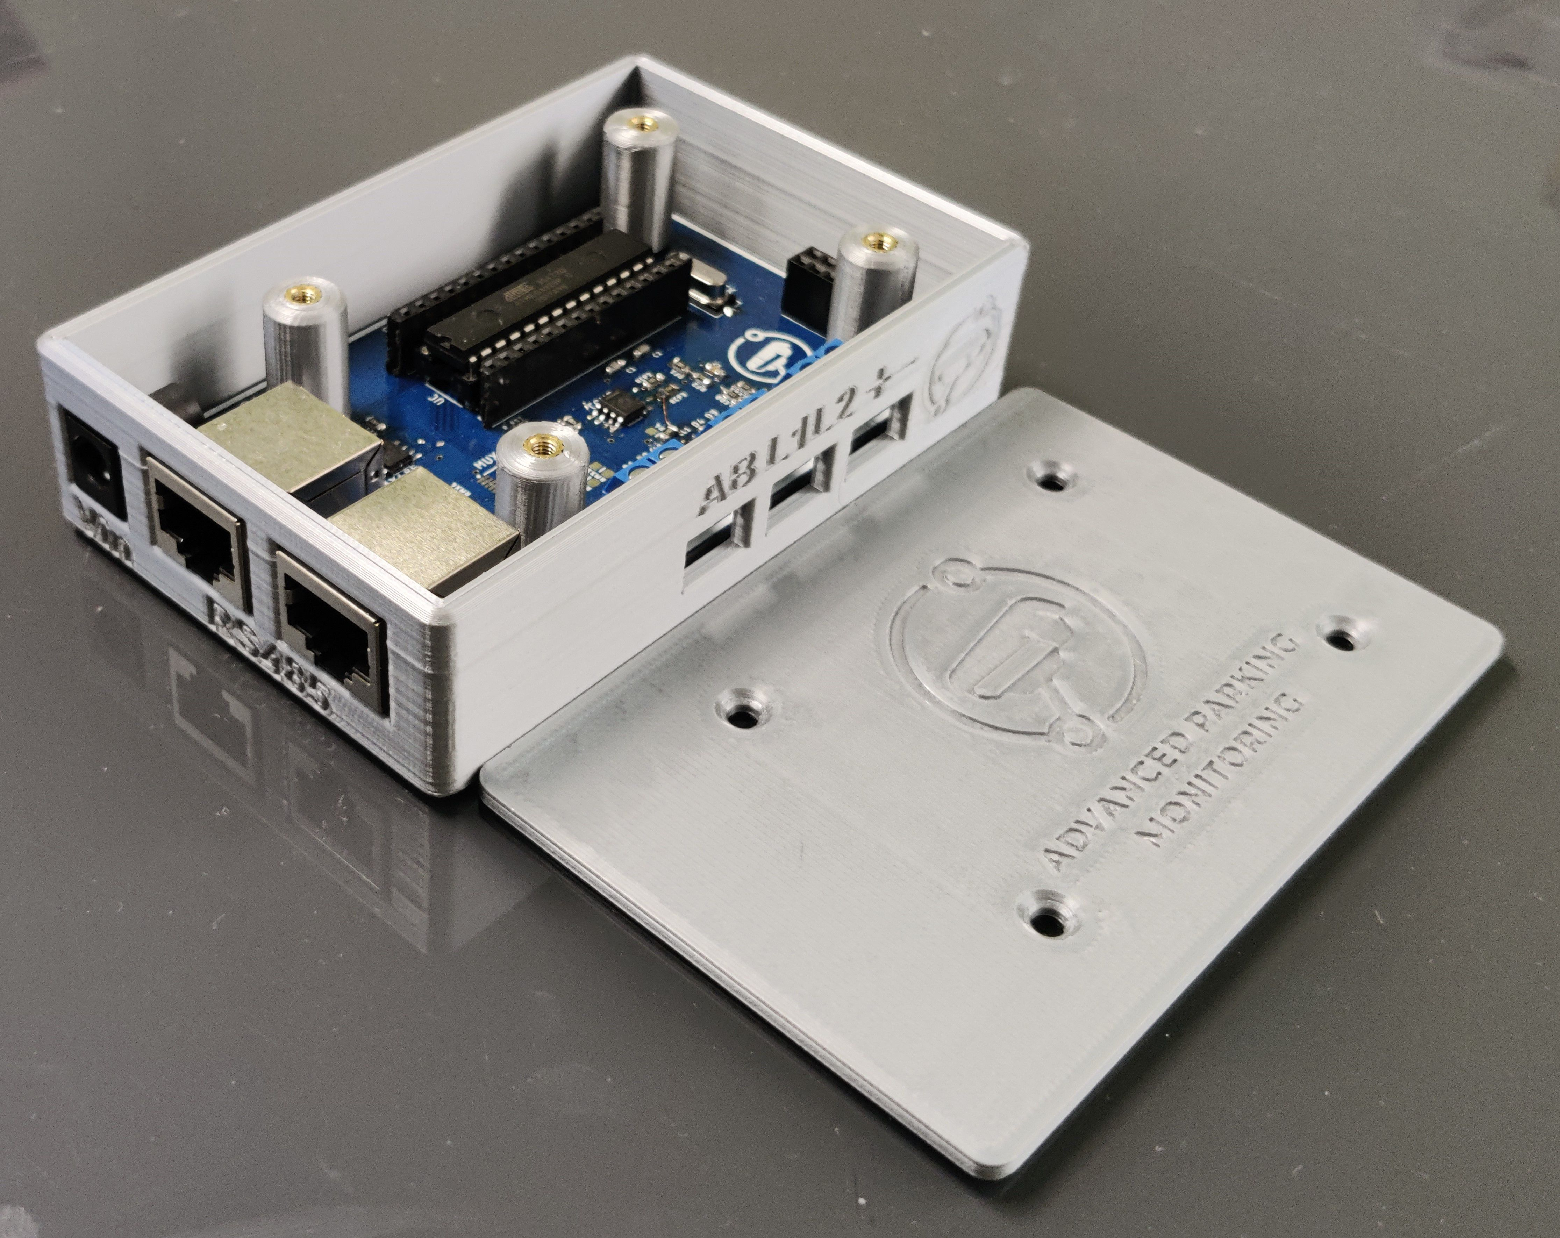
\includegraphics[width=0.6\linewidth]{fahrzeugerkennung/prototype1.pdf}
    \caption{erster Slave Prototyp}
\end{figure}

Um einzelne Fehler auszubessern und um weitere Eigenschaften anzubringen wurde im späteren
Verlauf eine weitere Version des Slaves erstellt. Diese Version ist im Vergleich zur letzten kleiner
und verwendet durchgehend SMD Varianten der ICs. In der unteren Abbildung sehen wir rechts
den alten Prototyp und links die neueste Version des Slaves.

\begin{figure}[H]
    \centering
    \includegraphics[width=0.6\linewidth]{fahrzeugerkennung/both_slaves.pdf}
    \caption{beide Slave Prototypen}
\end{figure}


\subsubsection{Gehäuse}\mbox{} 

Das Gehäuse wurde in Fusion360\footnote{\url{https://www.autodesk.de/products/fusion-360/overview}} erstellt um das Slave-Gerät besser vor Umwelteinflüssen zu schützen ohne dabei die Funktionalität des Gerätes einzuschränken. Es existieren insgesamt
drei Teile, die zusammenverschraubt das Gehäuse bilden. Das Material, welches verwendet wurde
ist ein 3D-druckbares PLA Polyester. Für die Gewinde wurden spezielle Gewindeeinsätze verwendet
mit einem metrischen Nenndurchmesser von 3 mm. Die verwendeten Schrauben entsprechen
der DIN-Norm 965.

\begin{figure}[!htb]
    \minipage{0.32\textwidth}
        \includegraphics[width=\linewidth]{fahrzeugerkennung/slave_boden.pdf}
        \caption{Boden des Slave Gehäuses}
    \endminipage\hfill
    \minipage{0.32\textwidth}
        \includegraphics[width=\linewidth]{fahrzeugerkennung/slave_wände.pdf}
        \caption{Wände des Slave Gehäuses}
    \endminipage\hfill
    \minipage{0.32\textwidth}%
        \includegraphics[width=\linewidth]{fahrzeugerkennung/slave_deckel.pdf}
        \caption{Deckel des Slave Gehäuses}
    \endminipage
\end{figure}

\subsection{USB-Master}
Die Aufgabe des Masters ist es die Kommunikation am Bus zu steuern, ihn mit Spannung zu versorgen und die Daten an das Webinterface weiterzugeben. 
In der folgenden Abbildung ist der logische Aufbau des Masters zu sehen.

\begin{figure}[H]
    \centering
    \includegraphics[width=0.6\linewidth]{fahrzeugerkennung/master_overview.pdf}
    \caption{Logischer Aufbau des Masters}
\end{figure}
\subsubsection{USB-Bussadapter Gerät}
\paragraph{FT232RL}\mbox{} 

Der FT232RL IC ist ein USB auf UART Wandler IC, der kein Programmieren des internen Speichers nötig hat. Er kann ohne weiteres über einen USB-Stecker an einen Computer angeschlossen werden. 
Neben den für USB relevanten Anschlüssen besitzt der Chip zusätzliche Pins um mehrere Funktionen zu erfüllen. In seinem Datenblatt ist eine Beispielschaltung vorgegeben für die Verwendung eines RS485-Pegelwandlers.
\begin{figure}[H]
    \centering
    \includegraphics[width=1\linewidth]{fahrzeugerkennung/ft232_rs485_datasheet.pdf}
    \caption{Beispielschaltung eines FT232 mit einem RS485 Pegelwandlers}
    \citeurl{ft232r_rs485}
\end{figure}

In der folgenden Abbildung ist der FT232 im Schaltplan des Busadapters dargestellt. Es sei zu beachten, dass die LEDs falsch angeschlossen sind. Die Anschlüsse CBUS0 und CBUS1 funktionieren als Stromsenken. 
Der Fehler wurde mittels Drahtbrücken und Umplatzierung der Bauteile korrigiert.
\begin{figure}[H]
    \centering
    \includegraphics[width=0.8\linewidth]{fahrzeugerkennung/ft232_schematic.pdf}
    \caption{FT232RL im Schaltplan}
\end{figure}

\paragraph{USB-C Anschluss}\mbox{} 

Als USB-Stecker ist der Typ C aufgrund seiner besonderen Eigenschaften ausgewählt worden. Er ist geometrisch sehr klein und symmertrisch seiner Drehachse entlang des Kabels. Im Vergleich zum Typ A oder Typ B Stecker 
kann man ihn nicht verkehrt einstecken. Aufgrund dieser Symmetrie besitzt er alle Anschlüsse doppelt. Die Anschlüsse im Schaltplan sehen wie folgt aus.

\begin{figure}[H]
    \centering
    \includegraphics[width=0.8\linewidth]{fahrzeugerkennung/usbc_schematic.pdf}
    \caption{USB Typ C Stecker im Master Schaltplan}
\end{figure}

Es werden nur die normalen D+ und D- Pins verwendet. Damit das USB-Gerät am anderen Ende weis, dass das Gerät für die serielle Kommunikation zur Verfügung steht sind zwei $\SI{5}{\kilo\ohm}$ an den Pins VCONN und CC nötig.

\paragraph{Layout des Master-Geräts} \mbox{} 

Genau gleich wie das Layout des Slaves wurde dieses in Eagle erstellt. Es gibt den zuvor erwähnten USB Typ C Stecker, einen RJ45 Anschluss für das Bussystem und einen Anschluss für eine Netzteil mit $\SI{9}{\volt}$ bis 
$\SI{30}{\volt}$.

\begin{figure}[H]
    \centering
    \includegraphics[width=0.6\linewidth]{fahrzeugerkennung/master_irl.pdf}
    \caption{USB-Bussadapet mit Gehäuse}
\end{figure}

\paragraph{Gehäuse}\mbox{} 

Das Gehäuse ist wie das Slave-Gehäuse in Fusion360 gezeichnet worden und mit einem 3D-Drucker ausgedruckt worden. Es existieren insgesamt 3 Teile, die zusammen das Gehaüse bilden.
Die verwendeten Gewinde sind die gleichen Gewindeeinsätze wie bei Slave und es wurden die gleichen Schrauben nach DIN-Norm 965 verwendet.

\begin{figure}[!htb]
    \minipage{0.32\textwidth}
        \includegraphics[width=\linewidth]{fahrzeugerkennung/master_boden.pdf}
        \caption{Boden des Master Gehäuses}
    \endminipage\hfill
    \minipage{0.32\textwidth}
        \includegraphics[width=\linewidth]{fahrzeugerkennung/master_wände.pdf}
        \caption{Wände des Master Gehäuses}
    \endminipage\hfill
    \minipage{0.32\textwidth}%
        \includegraphics[width=\linewidth]{fahrzeugerkennung/master_deckel.pdf}
        \caption{Deckel des Master Gehäuses}
    \endminipage
\end{figure}
\subsubsection{Master Programm}

\paragraph{Erkennung des USB-Geräts}\mbox{} 

Um den Bus ansteuern zu können ist es zuerst nötig den Busadapter zu finden. Alle registierten Geräte die an einem COM-Anschluss hängen können eindeutig durch ihre VID und PID identifiziert werden. 
Es ist jedoch auch möglich mithilfe des Herstellers des Gerätes den richtigen COM-Anschluss zu finden. Der untere Code geht im Master Programm alle verfügbaren Geräte durch bis es eines mit dem richtigen Hersteller findet.
Infolge wird dann der entsprechende COM-Anschluss zurückgegeben.

\begin{listing}[H]
    \begin{minted}{python}
    def get_port_vidpid(vid_pid):
    vp = vid_pid.split(':')
    pid = vp[-1]
    vid = vp[0]
    for device in devices:
        if device.vid != None or device.pid != None:
            if format(device.vid,'x') == vid and format(device.pid, 'x') == pid:
                return device.device
                break
    \end{minted}
    \caption{Master Code zur Erkennung des USB-Bussadapters}
\end{listing}


\paragraph{Frequenzauslesung}\mbox{} 

Für die Frequenzauslesung muss der Master die Form des entsprechenden Datenframes beachten (siehe Abbildung \ref{fig:master_frame}). Er muss zusätzlich noch eine MEsszeit für den Slave angeben. Der Slave gibt jedoc nicht die gemessene
Frequenz zurück, sondern die Anzahl der Takte über dem vorgegebenen Zeitraum. Das folgende Unterprogramm gibt bei erfolgreicher Messung die gemessene Frequenz zurück und gibt bei einem Fehler einen Text in die Kommandozeile.


\begin{listing}[H]
    \begin{minted}{python}
    def get_frequency(adress:int, measure_time):
        temp = ser.timeout
        ser.timeout = measure_time * (2 /10)
        write_frame(adress = adress, controll = CTRL.GET_FRQ.value, argument_1 = measure_time)
        (s, data, error_sent, error_received) = read_frame(True)
        if error_received == ERROR.NONE:
            ser.timeout = temp
            try:
                return int(data,16) / (measure_time / 10)
            except:
                print(s)

        print(s)
        return -1
    \end{minted}
    \caption{Frequenzsteuerbefehl des Masters}
\end{listing}
\paragraph{Auswertung}\mbox{} 

Die Auswertung der Frequenz kann auf unterschiedliche Weise erfolgen. Die einfachste Variante ist es eine Detektion festzustellen, wenn die gemessene Frequenz von der eines leeeren Parkplatzes abweicht. Dies setzt vorraus, dass die Frequenz bei leerer 
Parklücke bekannt ist. Der untere Code detektiert eine prozentuelle Frequenzänderung und gibt je nach dem eine Ausgabe an die Kommandozeile und eine POST-Anfrage an das API.

\begin{listing}[H]
    \begin{minted}{python}
    def update():
        global timer_iterations
        print(timer_iterations)
        for adress in f_dict:
        frq = Serial.get_frequency(adress, 60)
        print(frq)
        if frq * df_relative > f_dict[adress]:
            print(post(adress, 1))
            print("detected\n")
        else:
            print(post(adress, 0))
            print("not detected\n")
        timer_iterations += 1
        threading.Timer(1.0, update).start()
    \end{minted}
    \caption{Detektionscode des Masters}
\end{listing}


\paragraph{API-Post}\mbox{}

Für den Post an das API ist ein API-Token nötig. Bei Detektion eines Fahrzeuges wird die Parklücke mit der entsprechenden Adresse als belegt gekennzeichnet. Der untere Code übernimmt die Adresse der Parklücke und den Detektionszustand und übergibt sie der API.
Eine Verbindung zum Internet ist jedoch nötig.

\begin{listing}[H]
    \begin{minted}{python}
    def post(adress: int, occupied: int) -> str:
        url = "http://dev.philipp-kraft.com/api/v1/lots/3/spots"
        payload = {'address': str(adress), 'occupied': str(occupied)}
        files = []
        headers = { 'Authorization': 'TOKEN' }
        response = requests.request("POST", url, headers=headers, data=payload, files=files)
        return response.text
    \end{minted}
    \caption{API Post Code des Masters}
\end{listing}


\subsubsection{Raspberry Pi als Mastergerät}
\paragraph{SSH Remote Zugriff} \mbox{} 

Um den Raspberry Pi besser zu Konfigurieren und verwalten zu können ist ein Zugriff aus der Ferne sehr praktisch. Eine Möglichkeit ist der Zugriff mit SSH über einen VPS. Dafür benötigen alle beteiligten Geräte Zugriff auf das Internet.
Der Raspberry Pi baut zuerst einen Reverse SSH Tunnel zum VPS auf, da man vom VPS auf den Raspberry Pi zugreigen will. Ein externer Benutzer greift über den VPS mit einer SSH auf den Raspberry Pi zu.

\begin{figure}[H]
    \centering
    \includegraphics[width=0.8\linewidth]{fahrzeugerkennung/vps.pdf}
    \caption{Zugriff über VPS}
\end{figure}
Für das Erstellen das Reverstunnel muss folgender Befehl beim Raspberry Pi ausgeführt werden. Dabei muss die IP-Adresse des VPS \textit{VPSIP} bekannt sei und es muss ein Umleitungsport \textit{VPSPORT} festgelegt werden.
\begin{listing}[H]
    \begin{minted}{shell}
    ssh -R VPSPORT:localhost:22 Nutzer@VPSIP
    \end{minted}
    \caption{Öffnen des Reverse SSH Tunnels}
\end{listing}

Der externe Nutzer kann mit dem untenstehenden Befehl sich beim Benutzer \textit{pi} über SSH einloggen.

\begin{listing}[H]
    \begin{minted}{shell}
        ssh -p VPSPORT pi@VPSIP -o StrictHostKeyChecking=no
    \end{minted}
    \caption{Zugriff uf den Raspberry über SSH}
\end{listing}




\paragraph{Code Deployment} \mbox{} 

Für die Entwicklungsphase ist es sehr angenehm den fertigen Code auf den Raspberry Pi hinaufladen zu können. Github hat eine gewisse Funktionalität names Github Actions. Mit diesen kann bei einer bestimmten Aktion ein Linux-Server gestartet werden, der je nach
Anwendung bestimmte Shell-Befehle durchführt. Mit diesem Linux-Server lässt sich auch über SSH auf unseren Raspberry Pi zugreifen. Der untenstehende Befehl aktulisiert das lokale Repository des Raspberry Pi über SSH. Github brauch dafür diverse Daten wie das Kennwort
das Benutzers 'pi', die nicht in Klartext im Code stehen dürfen. Sie können als sogenannte Respository-Secrets deklariert werden. Aus diesen Grund steht im unteren Befehl nicht etwa die IP des VPS sondern secrets\_VPSHOST.  

\begin{listing}[H]
    \begin{minted}{shell}
    sshpass -p ${{ secrets.USER_PASSWORD }} ssh -o StrictHostKeyChecking=no -p ${{ secrets.VPS_PORT }} ${{ secrets.USER }}@${{ secrets.VPS_HOST }} \
        "cd /home/pi/Advanced_Parking_Monitoring_Raspberry_Master \
        && sudo git checkout . \
    \end{minted}
    \caption{Zugriff uf den Raspberry über SSH}
\end{listing}

Bei erfolgreicher Github Action sieht kann man folgendes in der Benutzeroberfläche von Github sehen.

\begin{figure}[H]
    \centering
    \includegraphics[width=0.8\linewidth]{fahrzeugerkennung/github action.pdf}
    \caption{Github Action im Github Master Repository}
\end{figure}


\pagebreak


